\documentclass[a4paper,UTF8,fontset = windows]{ctexbook}
\usepackage[margin=2cm]{geometry}
\usepackage{xeCJKfntef}
\usepackage{float}
\usepackage{amsmath}
\usepackage{mathtools}
\usepackage{amsfonts}
\usepackage{amssymb}
\usepackage{float}
\usepackage{tikz}
\usetikzlibrary{patterns}
\usepackage[
  pdfborder=0 0 0,
  bookmarksnumbered=true
]{hyperref}
\usepackage[user=student]{cexam}
\includeonly{%
  自序,
  chapter-统计物理学的基本原理,
  chapter-热力学量,
  chapter-巨正则分布,
  chapter-量子力学中的微扰论,
  Schwinger表象,
  chapter-国际制和高斯制的换算,
  chapter-经典力学,
  chapter-非理想气体,
  chapter-溶液,
  chapter-化学反应,
  chapter-涨落,
  chapter-二次量子化,
  chapter-狭义相对论,
}%
\begin{document}
\newcommand{\diff}{\,\mathrm{d}}%数学微分算子
\newcommand{\difh}{\mathrm{d}}%使用在微分中的算子

%\title{理论物理学习笔记}
%\author{冯振华}
%\date{2019/03/15}
%\maketitle
\tableofcontents
2018年我参加了研究生考试,成绩出来后较去年有所提升,但是仍然不理想,勉强达到可调剂的分数.但是我没有选择调剂,综合考虑后我还是执著的坚持再考虑一年.在2018的的考研准备工作中,由于要同时任教高中四个班级的物理课,我没有大量的时间像在校大学生一样做题,这是我不够熟练的第一个原因.同时,对于统计物理学概念理解的不深入,对于电动力学的理解也不是足够深入,这是第二个原因.英语一直是我的弱项,多少年来,我一直努力去学习它,但是收效甚微,可能是我对于这个学科不是太过敏感吧,在2019年的工作中,我一定要坚持下来学习英语,以期在2019年,顺利通过考试.

在学习的过程中,有些概念和计算理解起来有一定的难度,这也是学习过程中的核心,所以我计划在学习过程中按照自己的理解,使用\LaTeXe{}整理下来,以方便我今后的学习.在参考了大量的书籍后,我发现朗道的《理论物理教程》共十卷,很适合我的要求,所以坚持以它为主教材,然后在精读一遍后再做一些习题来应对2019年的研究生考试,不怕任何困难,相信自己一定能够实现自己的理想.

\chapter{统计物理学的基本原理}
\section{统计分布}
\subsection{平均值的表示}
用字母加上横线$\overline{f}$或尖括号$<f>$表示平均值,其中第二种方法对于表达书写繁冗表达式的平均值是极为方便的.这是和量子力学相一致的,最初我学习量子力学参加北京大学的理论物理考试时,都不能正确的识别这些符号,所以记录一下.
\subsection{统计平衡}
统计平衡也称为\CJKunderwave{热力学平衡}或\CJKunderwave{热平衡}状态.闭合宏观系统在其所处的状态下,其\CJKunderwave{任何子系统的宏观物理量}都充分精确地等于相应量的平均值的状态.
\subsection{弛豫时间}
一个离开平衡状态的系统过度到平衡状态所需要的时间称为\CJKunderwave{弛豫时间}.这里是描述此系统的所有物理量都达到稳定,所以弛豫时间应该就是所有物理量不再发生变化时的最长时间.平时所说``足够长''的时间实质就是比弛豫时间长得多的时间间隔.
\subsection{动理学}
与过渡到平衡状态有关的过程理论.
\section{统计独立}
\subsection{准闭合}
子系统与周围部分发生相互作用的主要是那些在子系统表面附近的粒子.这些粒子的数目与子系统中粒子的总数之比随着子系统尺度的增加而迅速下降,因而当子系统足够大时,它与周围部分相互作用的能量比子系统的内能要小的多.因此可以说子系统是{\color{red}准闭合}的.
\subsection{统计独立性}
一个子系统所处的状态绝不影响其它子系统处于不同状态的概率.其统计分布函数满足
\begin{equation}
  \rho_{12}=\rho_1\rho_2
\end{equation}
如果二个物理量是统计独立的,则
\begin{equation}
  \overline{f_1f_2}=\overline{f_1}\cdot\overline{f_2}
\end{equation}
\subsection{均方根涨落}
\begin{gather}
  <(\Delta f)^2>=<(f-\overline{f})^2>\notag\\
  <(\Delta f)^2>=<f^2-2\overline{f}f+\overline{f}^2>\notag\\
  <(\Delta f)^2>=<f^2>-2<\overline{f}f>+\overline{f}^2\notag\\
  <(\Delta f)^2>=<f^2>-2\overline{f}^2+\overline{f}^2\notag\\
  <(\Delta f)^2>=\overline{f^2}-(\overline{f})^2
  \intertext{所以均方根涨落为}
  \sqrt{<(\Delta f)^2>}=\sqrt{\overline{f^2}-(\overline{f})^2}
\end{gather}
\subsection{相对涨落}
相对涨落的定义为
\begin{gather}
  \frac{\sqrt{<(\Delta f)^2>}}{\overline{f}}
\end{gather}
\subsection{相对涨落与粒子数的平方根成反比}
\begin{gather}
  \intertext{设$f$为\CJKunderwave{可加的物理量}高物体分成数目很大的N个大致相同的部分,则}
  \overline{f}=\sum_{i=1}^N\overline{f}_i
  \intertext{由于统计独立性可得}
  <(\Delta f)^2>=<(\sum_{i=1}^N\Delta f_i)^2>=\sum_{i=1}^N<(\Delta f_i)^2>
  \intertext{则有}
  \frac{\sqrt{<(\Delta f)^2>}}{\overline{f}}\propto \frac{\sqrt{N}}{N}=\frac{1}{\sqrt{N}}
\end{gather}
\section{刘维定理}
一个闭合的系统设它的自由度为2s,使用分析力学来描述的时候符合Lagrange方程或Hamilton方程,所以在时刻t只要指明它的s个坐标和s个动量,则表明了一个状态.设$t_1$,$t_2$,$t_3$,$\cdots$ 的时刻的代表点用$A_1$,$A_2$,$A_3$,$\cdots$来表示,则经过足够长的时间后,由于系统的闭合性,则代表点总数是一定的.所以在$dpdq$的范围内,的代表点可以视为稳定的``气体'',因此符合连续性方程

\begin{gather}
  \frac{\partial\rho}{\partial t}+\frac{\partial \rho \dot{q}}{\partial q}+\frac{\partial \rho \dot{p}}{\partial p}=0
  \intertext{上式用微分原则展开则}
  \frac{\partial\rho}{\partial t}+\frac{\partial \rho }{\partial q}\dot{q}+\frac{\partial \rho }{\partial p}\dot{p}+
  \rho\left\{\frac{\partial \dot{q}}{\partial q}+\frac{\partial \dot{p}}{\partial p}\right\}=0
  \intertext{上式即}
  \frac{d\rho}{dt}+
  \rho\left\{\frac{\partial \dot{q}}{\partial q}+\frac{\partial \dot{p}}{\partial p}\right\}=0
  \intertext{根据Hamilton方程,得}
  \dot{p}=-\frac{\partial H}{\partial q} \qquad \dot{q}=\frac{\partial H}{\partial p}
  \intertext{所以有}
  \frac{d\rho}{dt}=0
\end{gather}

\section{能量的作用}

如果在一个相当长的时间段内观察一个严格闭合的系统,它是稳定的,所以总的代表点数不会发生变化,在初值给定后,从单纯的力学角度考虑,相轨道一定是闭合的,系统具备一定的周期性,这个周期可以视为系统的弛豫时间.如果系统的相轨道不是闭合的,则系统的总代表点数必然是无限多个,这是不实际的.刘维定理所回答的是代表点密度是不随时间变化的常数,但是它不能回答的是对于不同的初始值,这个$\rho$值是否是相同的,这就需要从统计的角度考虑,由于不能说明哪一个初始值更具有特殊性,所以平均看来不同初始值的点这个$\rho$值应当是相同的.
\begin{gather}
  \intertext{考虑两个闭合系统构成的一个大系统,这个大系统也处于平衡状态,则有} 
  \rho=\rho_1\rho_2
  \intertext{取对数则}
  \ln\rho=\ln\rho_1+\ln\rho_2
  \intertext{上式表明,$\ln\rho$是一个可加性的积分常数.所以在相对于质心静止的坐标系中,这个值仅仅依赖于能量,即}
  \ln\rho=\alpha+\beta E
  \intertext{式中$\alpha$是一个可加性的量,依赖于归一化.由于能量$E$也是一个可加性的量,所以处于平衡状态的系统它们的$\beta$值是相同的.}\notag
\end{gather}

在朗道的书\footnote{《朗道理论物理教程 卷5 统计物理学1》第10页}中写到:上面的讨论可以使我们直接构造出一个适于描述系统统计性质的简单的分布函数.我们现在既然知道不可相加的运动积分的值不会对系统的统计性质发生影响,那么任何函数$\rho$只要它依赖于系统的可加性运动积分的值,并且满足刘维尔定理,就可以用来描述闭合系统的统计性质.最简单的这种函数就这样一个函数:{\color{red}在相空间中,对于所有的相应于系统的能量、动量和角动量取给定常数$E_0$,$P_0$,$M_0$的点,$\rho=\mbox{常数}$(不依赖于非可加性运动积分的值),对于所有其它的的点,$\rho=0$}.显然,这样规定的分布函数在任何情况下沿着系统的相轨道都保持常数,即满足刘维尔定理.

上述红字部分,是朗道所做的规定,但是理由没有做详细的讨论,这实际是汪志诚《热力学与统计物理学》中所述的,基于统计的考虑:等概率原理.这也可以做如下考虑:两个存在相互作用的系统构成一个大的系统,则每一个部分以及整个大的闭合系统处于平衡状态,则系综的分布函数仍然具备乘积的形式,即$\rho=\rho_1\rho_2$.但是两个小部分是存在相互作用的,它们不是严格的闭合系统,但是可以认为相互作用足够小,而认为它们是准闭合的系统.则基于能量在相互作用非常微弱的情况下,可以认为满足可加性的,则分布函数就可以认为是满足可加性的.这个考虑是可靠的,因为一个宏观无穷小,微观无穷大的系统,相互作用的能量是远小于子系统的总能量的.

\subsection{微正则分布}

在相空间中,凡是$E$,$P$,$M$这些量中有一个不等于它们的给定值$E_0$,$P_0$,$M_0$的那些点,$\rho$为零点.函数$\rho$对于包含上述流形相点全部或部分在内的相体积求积分是有限的.则

\begin{gather}
  \rho= cost \cdot \delta(E-E_0)\delta(P-P_0)\delta(M-M_0)
  \label{eq:weizhengze}
\end{gather}

式\eqref{eq:weizhengze}称为\CJKunderwave{微正则分布}.特殊一个情况:设想把系统包藏在一个刚体的``匣子''中,并且所有的坐标系相对于``匣子''是静止的.则运动积分只剩下能量,则微正则分布变成更加简单的形式,仅依赖于能量

\begin{gather}
  \rho= cost \cdot \delta(E-E_0)
  \label{eq:weizhengze1}
\end{gather}

由力学运动积分及可加性物理量可得$\rho$和能量的函数关系为

\begin{gather}
  \ln\rho_n=\alpha_n+\beta E_n(p,q)
\end{gather}

\section{统计矩阵}
\subsection{量子力学中的密度矩阵}
\begin{gather}
  \intertext{设所研究的系统不是完全闭合的,所以它不具备自己的波函数.只能用系统的波函数计算平均值.则}
  \overline{f}=\int \Psi^*(x,q) \hat{f}\Psi(x,q)dqdx
  \intertext{令上式$\Psi^*$中的$x$替换为$x'$,然后$\hat{f}$就可以移到最前面,而后再对$q$积分便得到密度矩阵}
  \overline{f}=\int \hat{f} \int\Psi^*(x',q)\Psi(x,q)dqdx
  \intertext{令$\omega(x',x)=\int\Psi^*(x',q)\Psi(x,q)dq$,称为密度矩阵,则}
  \overline{f}=\int \hat{f}\rho(x',x)|_{x'=x}dx
  \label{eq:midu0}
\intertext{上式的意思是,先令$\hat{f}$作用到$\rho(x',x)$上,再令$x'=x$然后再对$x$积分,便得到$f$的平均值.令$\Psi$使用子系统的某一物理量的本征函数$\psi_n$展开,则}
\rho(x',x)=\sum_{n,m}\int C_m^*(q)C_n(q)dq\psi_m^*(x')\psi_n(x)
\intertext{令$\omega_{nm}=\int C_m^*(q)C_n(q)dq$,称为密度矩阵,则}
\rho(x',x)=\sum_{n,m}\omega_{nm}\psi_m^*(x')\psi_n(x)
\intertext{将上式代入\eqref{eq:midu0}得}
\overline{f}=\sum_{n,m} \omega_{nm}\int \psi_m^*(x)\hat{f}\psi_n(x)dx
\intertext{以矩阵元$f_{mn}=\int \psi_m^*(x)\hat{f}\psi_n(x)dx$代入上式,则}
\overline{f}=\sum_{n,m} \omega_{nm}f_{mn}
\intertext{以算符$\hat{\rho}$表示密度矩阵算符,则}
\overline{f}=\sum_{n}(\hat{\omega}\hat{f})_{nn} 
\intertext{上式也可以使用矩阵的迹表示为}
\overline{f}=tr(\omega f)
\end{gather}
\subsection{统计物理学中的密度矩阵}

\begin{gather}
  \intertext{仍然考虑一个由子系统和外界构成的闭合系统.则将波函数按子系统的某物理量的本征态展开.则}
  \Psi=\sum_n c_n \psi_n(q)
  \intertext{所以量子力学纯态中,坐标概率分布由波函数的模方来确定,即}
  |\Psi|^2=\sum_{n,m}C^*_n C_m \psi_n^* \psi_m
  \intertext{由于当子系统处于某一个能量状态时,介质的状态可能有多个,也就是上式中的系数对子系统在不同时刻是不同的,考虑一个较长的时间,系统经历了足够多的状态,则按系综求平均,则}
  |\Psi|^2=\sum_{n,m}\omega_{m,n} \psi_n^* \psi_m
  \intertext{对于某一物理量,可以求它的平均值}
  \overline{f}=\int \hat{f}|\Psi|^2 dx=\sum_{n,m}\omega_{m,n}f_{n,m} 
  \intertext{引入密度矩阵算符$\hat{\omega}$,根据矩阵的乘积运算,则}
  \overline{f}=\sum_n (\hat{\omega}\hat{f})_{n,n}
  \intertext{上式又可以写成矩阵的迹}
  \overline{f}=tr(\hat{\omega}\hat{f})
\end{gather}

在写这一部分时,出现了一点情况\footnote{在使用\LaTeX{}编译pdf文件时,出现了字体报错,这迫使我暂时离开去研究一下字体的问题。在ctex宏包手册中得到答案,安装字体后得到解决。同时处理这一部分,导致我解决了向pdf文件中加入目录outline的问题,那就是pdftk工具,同时加入中文目录可以使用\LaTeX{}编写章节,生成Pdf文件,再用pdftk提取目录,再导入到目标文件即可。},经过几天的研究,马上回到热统的学习过程中,记录自己的学习感想。

\subsection{概率密度和能量的关系}

%经典统计中,由于在相格内的状态不是一个,所以可以推断概率密度具备$\delta$函数的形式.但是量子系统,能量是分立的,不会出现类似的情况,但是子系统一般不是孤立的,也就是子系统的能量是有一定宽度的,所以需要引入能量满足此宽度$\Delta E$时的状态数,此状态数是能量波函数的个数,并不是具体到的一个简并态.则系统处于一个能量量子态的概率也就可以理解为概率密度.也就是

\begin{gather}
  \intertext{在量子力学中描述一个量子体系,如果在$q$表象中,则其值为$q$时的概率为}
  d\omega_q =\Psi^2 dq
\intertext{对于一个闭合的系统,则密度矩阵是对角的,但是对角元是所取表象中某一量子态出现的概率.此时能级是无限稠密的,由于系统与外界存在相互作用,所以它的能量是有一定宽度的,所以可以选择能量小于某个值 $E$ 的各个量子态作为一个表象,同时由于在统计中能量决定了各量子态的分布,所以用各个量子态作为表象也是相对"完备"的,于是 \CJKunderwave{在 \mbox{$E$}\mbox{$\sim$}\mbox{$E$}+\mbox{$\Delta E$} 中的任何一个量子态的概率为}}
  d\omega =\Psi^2 d\Gamma
\intertext{同时由于系统还要受能量的限制,所以自由度会减少,则几率密度必然呈显 $\delta$ 函数的性质,则 \CJKunderwave{在 \mbox{$E$}\mbox{$\sim$}\mbox{$E$}+\mbox{$\Delta E$} 中的任何一个量子态的概率}形式上可以取为}
  d\omega=\mbox{常数}\cdot \delta(E-E_n)d\Gamma
  \intertext{如果系统的各个部分构成的小子系统处于准闭合状态,则上式的量子数又可以表达为 $d\Gamma=\prod_\alpha d\Gamma_\alpha$ ,但是各个子系统的能量和必须满足位于$E\sim E+\Delta E$ 中}
  d\omega=\mbox{常数}\cdot \delta(E-E_n)\prod_\alpha d\Gamma_\alpha
\end{gather}


\section{熵}

\subsection{熵的定义}

系统在$E\sim E+\Delta E$内的微观状态数,记为$\Delta\Gamma$,则熵的定义为

\begin{equation}
  S=\ln \Delta\Gamma
  \label{eq:shang}
\end{equation}

需要注意的是,在此处的定义和经典Boltamann关系$S=k\ln\Omega$不同,原因在于单位的选择上,它是温度所取单位为$erg$时的表达式,特点是简洁,后面的推证会给出说明.在朗道的书中直接结出这个定义,我认为从很大程度上给出了解决问题的核心,是一个相当好的设置.

在经典统计中,没有量子态的概念,但是可以引入Plank常数来处理.根据量子力学测不准原理,能够同时指明坐标和动量的限度就是一个Plank常数,所以对应经典统计熵的定义就是

\begin{equation}
  S=\ln\frac{\Delta p\Delta q}{(2\pi\hbar)^s} 
  \label{eq:shang1}
\end{equation}

\subsection{熵和分布函数的关系}
\begin{gather}
  \intertext{对分布函数关于全部状态求积分,则总概率一定为1,则}
  \int \omega(E)d\Gamma=1
  \intertext{考虑到分布函数和能量的关系,它具备$\delta$函数的性质,则记分布函数最大时,能量$\overline{E}$,则上式可以写为}
  \omega(\overline{E})\Delta \Gamma=1
  \intertext{对上式取对数得}
  \ln\Delta\Gamma=-\ln\omega(\overline{E})
  \intertext{于是得熵和分布函数关系为}
  S=-\ln\omega(\overline{E})
\end{gather}


\subsection{熵的可加性}
\begin{gather}
  \intertext{当两个系统构成一个大的系统时,在各自准闭合的情况下,微观状态数关系为}
  \rho=\rho_1\rho_2
  \intertext{取对数再取负号,则}
  -\ln\rho=-\ln\rho_1-\ln\rho_2
  \intertext{即按熵和分布函数关系得}
  S=S_1+S_2
\end{gather}

\section{关于经典统计和量子统计的思考}

\subsection{经典统计}

1.确定统计分布函数的存在.对于一个系统,观察足够长的时间$T$,则在$\Delta t$这一小段时间内处于相格$\Delta p\Delta q$内,则比值$\omega$接近一个常数,即
\begin{equation}
  \omega=\lim_{T\to\infty} \frac{\Delta t}{T}
\end{equation}

显然这可以看成是系统处于相格$dpdq$内的概率.在李政道所著《统计力学(讲义)》中按照系综理论也给出了说明\footnote{李政道讲义 统计力学/李政道编著.---上海:上海科学技术出版社,2006.11第7页.}:所设想系综的总数为$M$ , 所有系综的总能量为$E$ ,当所取系综增加时,总能量也增加,但是比值$\frac{E}{M}$越来越趋于一个稳定值,这就是系统的能量,这也说明了当系综取的足够多时,系统会有一个确定的分布,这也说明了统计分布函数的存在.

2.系统处于相空间内的概率.

\begin{equation}
  d\omega=\rho dpdq
\end{equation}

3.考虑一们准闭合的系统,在足够长的一段时间内,沿某一相轨道运动其符合经典运动规律.在$\Delta t$内,$t_i$时刻系统的代表点为$A_i$,则在经典意义上,这样的态可以有无限多个.但是由于肯定了分布函数的存在,所以可以设想有和这些态同等数目的相同的系统,则每一时刻这些系统必处于其中的一个态中,由于随时间系统会演化,则相当于同一时刻这些不同的代表点相互转化,但是一定在所设想的所有态中.这些态,可以表达为坐标和动量的函数.所以分布函数的存在说明,$\Delta p\Delta q$内的代表点总数是不随时间变化的.这个考虑可以将这些代表点视为一些稳定存在的气体,但是还不能肯定的是一个足够小的区间内代表点的变化情况,也就是代表点密度问题没有得到解答.由于总数一定,所以代表点的变化一定符合连续性方程,再结合Hamilton方程就可以得到刘维定理,这定理肯定了代表点密度不随时间变化.

4.按朗道的说法,只要观察时间足够短,则系统就可以看成准闭合的系统,则符合经典运动规律.则分布函数不会发生变化,但是若在所观察的时间内,恰好系统受到了一个微小的干扰,系统由一个经典轨道恰好跳到另一个轨道上,这时代表点密度是否会发生变化呢?这就需统计的考虑,不应当认为哪一个轨道是特殊的,所以就能肯定这两个代表点密度也是相同的.所以就肯定了,准闭合的系统其受到外界稍微干扰后仍然满足等概率原理.

5.系统处于能量$E\sim E+\Delta E$的分布函数应当也满足$\delta$函数的形式,因为不处于相格内的状态出现的概率为零,但是按等概率原理,处于这个相格内的分布函数可以视为常数\footnote{按朗道的说法,只要是满足刘维定理的函数原则上都可以选为分布函数,只不过常数是一个最简单的情况.},同时系统的动量和坐标所构成的是$2s$维相空间,但是除此之外还要受到能量的限制,所以实际的自由度应该小于$2s$,因此在微正则分布中分布函数只有满足$\delta$函数的形式才能保证总概率不为零.即

\begin{equation}
  \rho =const \cdot \delta(E-E_0)
\end{equation}

\subsection{量子统计}

在量子统计中,一个子系统的状态要按密度矩阵来描述.由于所考虑的宏观物理量是稳定的,所以它们应当与Hamilton量对易,这就表明,这些物理量和能量表象具备相同的本征态.,所以其平均值可以记为

\begin{equation}
  \overline{f}=\sum_n \omega_nf_{nn}
\end{equation}

同时分布函数也是稳定的,则它也与Hamilton量对易,则表明矩阵$\omega$也是对角的.则$\omega_n$由上式可得就表示能量本征态$\psi_n$出现的概率.这构成了量子统计的基础.

对于量子系统,由于它不像经典的连续谱一样,所以谈不上系统处于相格内的状态数这一概念,但是对比经典统计,我们可以说这个分布函数就是一个状态上的概率,所以它也具备$\delta$函数的性质,但是处于能量$E\sim E+\Delta E$的能量状态,按统计的考虑,说不上哪一个 是特殊的,所以也等概率原理这些状态出现的概率是相同的,系统处于这个能量范围的概率为$d\omega$,则系统处于一个能量状态上的概率为

\begin{equation}
  \frac{d\omega}{d\Gamma}=const\cdot \delta (E-E_n)
\end{equation}

\section{熵的统计表达式}

\begin{gather}
  \intertext{基于准闭合系统能量可加性得到了分布函数和能量的关系}
  \ln\omega(E)=\alpha+\beta E
  \intertext{同时对上式求平均,则}
  <\ln\omega(E)>=\alpha+\beta\overline{E}
  \intertext{同时,基于函数关系也有}
  \ln\omega(\overline{E})=\alpha+\beta \overline{E}
  \intertext{对比可知}
  <\ln\omega(E)>=\ln\omega(\overline{E})
  \intertext{考虑到熵和分布函数的关系,则}
  S=-<\ln\omega(E)>
  \intertext{上式也可以写为}
  S=-\sum_n(\omega\ln\omega)_{n,n}
  \intertext{用矩阵的迹表达为}
  S=-tr(\omega\ln\omega)
\end{gather}
\section{量子力学基本原理}

\begin{gather}
\intertext{一个系统,如果我们可以在多次测量中确定某一个物理量$f$,用n表示它的量子数,则对于\CJKunderwave{不同的该物理量的值},用不同的态函数$\psi_n$来表示.则波函数满足线性叠加原理,则}
\Psi=\sum_n C_n\psi_n
\label{eq:biaoxiang0}
\intertext{其中$C_n^2$是测得该物理量的值的概率.但是此时能获得的信息就是$f$,如果又发现在$f$所区分的这些态下,物理量$p$还有不同的值,则可以说$f$相对于$p$而言是简并的.从数学上不难理解,$f$的态,可以用$p$的不同本征态$\varphi_m$来表示,即}
\psi_n=\sum_m a_m\varphi_m
\label{eq:biaoxiang1}
\intertext{将式\eqref{eq:biaoxiang1}代入式\eqref{eq:biaoxiang0}则得到体系的态函数的更加详细的表达式}
\Psi=\sum_n \sum_m C_na_m\varphi_m
\intertext{以$\omega_{mn}=C_na_m$和$\phi_{mn}=\varphi_m$作符号上的替换,则}
\Psi=\sum_{mn}\omega_{mn}\phi_{mn}
\intertext{按统计诠释,则$\omega_{mn}^2$表示体系处于态$\Psi$的描述时,同时测得物理量$f$和$p$的值分别为$f_n$和$p_m$时的概率.如果再发现一个物理量在$f$和$p$同时具备一定值时,它也具备定值,则我们说使用物理量$f$和$p$来描述系统是不完备的,所以当再追加一个物理量$q$后再也找不到这种同时可以测定的物理量后,人们说使用物理$f$,$p$,$q$来描述系统是完备的.如果将量子力学用于描述一个系统,则在空间中描述要解Schr\"odinger方程,所以会出现三个量子数:主量子数n,角量子数l,角动量在z轴的分量$l_z$,所以描述一个三维空间的物体系统,在经典力学下需要三个坐标,如果描述一个量子系统,则需要三个对易的物理量才能描述系统,物理量的数目应当与空间的维度相一致.但是在这里需要注意,采用这个描述是在认为质心不变的情况下描述的.如果在质心以外的参考点来描述系统需要指明质心的位置,也就是需要三个坐标,同时还要指明系统相对于质心的运动这就需要追加它相对于质心的角量子数及其相对于过质心的轴的方向上角量子数的投影,这正是自旋的来源.对于基本粒子,由于其内部结构无法继续深入研究探明,所以只能精确到这种程序.如果能够确认电子等基本粒子还有内部结构,则还需要追加自由度.下面用Dirac符号来表达自旋的影响但是在这里需要注意,采用这个描述是在认为质心不变的情况下描述的.如果在质心以外的参考点来描述系统需要指明质心的位置,也就是需要三个坐标,同时还要指明系统相对于质心的运动这就需要追加它相对于质心的角量子数及其相对于过质心的轴的方向上角量子数的投影,这正是自旋的来源.对于基本粒子,由于其内部结构无法继续深入研究探明,所以只能精确到这种程序.如果能够确认电子等基本粒子还有内部结构,则还需要追加自由度.下面用Dirac符号来表达自旋的影响.原本系统处于某一个态$\Psi$,则}
|\Psi>=\sum_{nlm}|nlm><nlm|\Psi>
\label{eq:biaoxiang2}
\intertext{而电子的自旋为$\hbar$,其在$z$轴方向上的投影只能是$\pm\frac{1}{2}$,所以相当于在上术波函数中每一个波函数还可以按自旋量子数展开,则}
|\Psi>=\sum_{nlm}|\frac{1}{2}><\frac{1}{2}|nlm><nlm|\Psi>+\sum_{nlm}|-\frac{1}{2}><-\frac{1}{2}|nlm><nlm|\Psi>\\
|\Psi>=|\frac{1}{2}><\frac{1}{2}|\Psi>+|-\frac{1}{2}><-\frac{1}{2}|\Psi>
\intertext{同时如由于电子的自旋数为$\hbar$这是确定的,所以在波函数中不需再单独说明,而只指明它的$z$分量就可以了,则}
|\Psi>=\sum_{nlm}|nlm\frac{1}{2}><nlm\frac{1}{2}|\Psi>
+\sum_{nlm}|nlm-\frac{1}{2}><nlm-\frac{1}{2}|\Psi>
\end{gather}


\chapter{热力学量}

\section{热力学不等式}

\hfill 2019年 03月 29日 星期五 21:23:13 CST
\begin{gather}
  \intertext{设想由物体和介质构成的一个大系统,则总熵记为$S_t$,系统的熵记为$S$.介质的熵记为$S_0$,则由于系统比介质小的多,而介质可以认为保持压强和温度不变,所以对于系统可以列出能量守恒定律,即}
  \Delta E=W+P_0\Delta V_0-T_0\Delta S_0
  \label{eq:lexiatalie0}
  \intertext{由于总系统的体积保持不变,且有熵增原理,则}
  \Delta V+\Delta V_0=0 \quad \Delta S+\Delta S_0 \geqslant 0
  \label{eq:lexiatalie1}
  \intertext{将式\eqref{eq:lexiatalie1}代入式\eqref{eq:lexiatalie0}得}
  W\geqslant \Delta E +P_0 \Delta V-T_0\Delta S
  \intertext{式中$W$表示客体对系统做的功,而系统对客体做的功应当与它相差一个负号,所以客体对系统做的最小功为}
  W_{min}=\Delta E +P_0 \Delta V-T_0\Delta S
  \intertext{如果没有客体做功,则系统和介质构成一个闭合的孤立的大系统,其也符合熵增原理,则}
  0 \geqslant \Delta E +P_0 \Delta V-T_0\Delta S
  \label{eq:lexiatalie2}
  \intertext{系统的能量是其熵和体积的函数,则考虑其Taylor 展开的二级项,则}
  dE=\frac{\partial E}{\partial S}dS+\frac{\partial E}{\partial V}dV+\frac{1}{2}
  \left\{
    \frac{\partial^2E}{\partial S^2}dS^2+2\frac{\partial^2E}{\partial S\partial V}dSdV+\frac{\partial^2E}{\partial V^2}dV^2
  \right\}
  \label{eq:lexiatalie3}
  \intertext{上式即}
  dE-T\Delta S+P\Delta V=\frac{1}{2}
  \left\{
    \frac{\partial^2E}{\partial S^2}dS^2+2\frac{\partial^2E}{\partial S\partial V}dSdV+\frac{\partial^2E}{\partial V^2}dV^2
  \right\}
  \label{eq:lexiatalie4}
  \intertext{式\eqref{eq:lexiatalie2}反映的是一个系统在不平衡时所能自发进行的过程,当它再次达到平衡,则熵又达到最大,所以就会有下式成立}
  \Delta E -T_0\Delta S+P_0 \Delta V > 0
  \intertext{\eqref{eq:lexiatalie4}代入上式可得}
  \frac{1}{2}
  \left\{
    \frac{\partial^2E}{\partial S^2}dS^2+2\frac{\partial^2E}{\partial S\partial V}dSdV+\frac{\partial^2E}{\partial V^2}dV^2
  \right\} > 0
  \label{eq:lexiatalie5}
  \intertext{上式如果成立,则必有}
  \left\{
    \begin{gathered}
      \frac{\partial^2E}{\partial S^2}>0 \quad \frac{\partial^2E}{\partial V^2}>0\\
      \frac{\partial^2E}{\partial S^2}\frac{\partial^2E}{\partial V^2}-\left(
      \frac{\partial^2E}{\partial S\partial V}\right)^2>0
    \end{gathered}
  \right.
  \intertext{上式也即}
  \left\{
    \begin{gathered}
      \frac{T}{C_v}>0 \quad \left(\frac{\partial P}{\partial V}\right)_T<0\\
      \frac{\partial^2E}{\partial S^2}\frac{\partial^2E}{\partial V^2}-\left(
      \frac{\partial^2E}{\partial S\partial V}\right)^2>0
    \end{gathered}
  \right.
\end{gather}

\section{能斯特定理}

在 \S 23 能斯特定理的第23.4 式的说明中提到从 16.9 式看出来.但是我仔细考察了这个问题,发现不是一眼能看出来,所以放到这里来论述一下.第 23.4 式为

\begin{gather}
  \mbox{当 $T=0$ 时 ,} \quad \frac{C_p-C_v}{C_p}=0.
\end{gather}

当熵 $S$ 按某种幂律变为零时,即 $ S=aT^n$ 其中 $a$ 为 $V,P$ 的函数.则

\begin{align}
  \left(\frac{\partial V}{\partial T} \right)_p &=-\left(\frac{\partial S}{\partial P} \right)_T=-\frac{\partial a}{\partial P} \cdot T^n
  \label{eq:nst0}\\
  \left(\frac{\partial P}{\partial T} \right)_v &=\left(\frac{\partial S}{\partial V} \right)_T=\frac{\partial a}{\partial V} \cdot T^n
  \label{eq:nst1}\\
  C_V&=T\left(\frac{\partial S}{\partial T}\right)_v=n\cdot aT^n
  \label{eq:nst2}\\
  \left(\frac{\partial V}{\partial P}\right)_T=\frac{\partial(V,T)}{\partial(P,T)}=&\frac{\partial(V,T)}{\partial(V,P)}\cdot \frac{\partial(V,P)}{\partial(P,T)}=-\left(\frac{\partial T}{\partial P}\right )_v\cdot \left(\frac{\partial V}{\partial T}\right)_p
  \label{eq:nst3}
\end{align}

由偏微分运算易得如下关系

\begin{gather}
  C_p-C_v=-T\frac{\left(\frac{\partial V}{\partial T}\right)^2_P}{\left(\frac{\partial V}{\partial P}\right)_T}
  \intertext{由式\eqref{eq:nst0}可知上式分子部分与 $T^{2n+1}$成正比,而分母部分由式\eqref{eq:nst3}可知与温度无关.所以有}
  C_p-C_v \propto T^{2n+1}
  \intertext{或者有关系}
  \frac{C_p-C_v}{C_p} \propto T^{n+1}
\end{gather}

\chapter{巨正则分布}
\section{配分函数}
\subsection{关于求和的讨论}
\begin{gather}
  \intertext{在近独立的情况求配分函数会出现如下形式的和}
  \sum_{a_n}e^{-\sum_n \varepsilon_n a_n}
  \intertext{为了方便讨论,我们取二项的情况讨论,形式如下}
  \sum_{a_1,a_2}e^{-\varepsilon_1a_1-\varepsilon_2a_2}
  \intertext{显然上述的和式可以表达为关于$\varepsilon_1$ 和 $\varepsilon_2$ 的某函数的乘积,同时基于二者的相同地位,则可以判断此函数结构相同,即}
  \sum_{a_1,a_2}e^{-\varepsilon_1a_1-\varepsilon_2a_2}=f(\varepsilon_1)\cdot f(\varepsilon_2)
  \intertext{由求和的结果可以判断每一项$f(\varepsilon_n)$应当包含所有属于 $\varepsilon_n$ 的指数项,即}
  f(\varepsilon_n)=\sum_{a_n}e^{-\varepsilon_n a_n}
\end{gather}

\subsection{近独立分布}
\begin{gather}
  \intertext{巨正则分布的配分函数表达为}
  \varXi =\sum_N e^{\frac{\mu N}{T}}\sum_{n}e^{-\frac{E_{nN}}{T}}
  \intertext{上式的求和是保持$N$不变先对能级求和,然后再对 $N$ 求和.在近独立的情况下此式可以推得广延量的相加性质.一个准闭合系统有}
  \begin{gathered}
    \sum_n a_n=N\\
    \sum_n \varepsilon_n a_n =E
  \end{gathered}
  \intertext{近独立的情况配分函数可以写为}
  \varXi =\sum_N \sum_{n}e^{\sum_n(\frac{\mu}{T}-\frac{\varepsilon_n}{T})a_n}
  \intertext{巨正则分布是计及了能量涨落和总粒子数涨落的,所以对 $N$ 的求和可以转化为对一切可能的 $a_n$ 求和,同时由上述表达式可得}
  \varXi = \prod_n \sum_{a_n} e^{\frac{\mu-\varepsilon_n}{T}\cdot a_n}
  \intertext{记上述和式为$\varXi_n$即}
  \varXi_n = \sum_{a_n} e^{\frac{\mu-\varepsilon_n}{T}\cdot a_n}
  \intertext{即}
  \varXi =\prod_n \varXi_n
  \label{eq:Xi0}
  \intertext{巨热力势函数为}
  \Omega = -T\ln \varXi
  \intertext{代入式\eqref{eq:Xi0}可得}
  \Omega = -T\ln \prod_n \varXi_n=\sum_n \Omega_n
  \intertext{其中 $\Omega_n$ 是和能级$ \varepsilon_n$ 相对应的巨热力势函数,即}
  \Omega_n = -T\ln \varXi_n
  \intertext{其中关于 $n$ 的求和就是对每一个能级的求和,如果某一能级有简并,如$\varepsilon_1$ 和 $\varepsilon_2$ 是相同的能级, 记为 $\varepsilon_1'$ 则 }
  \varXi_1'=\varXi_1\cdot \varXi_2=(\varXi_1)^2
  \intertext{则和能级 $\varepsilon_1$  对应的巨热力势函数 $\Omega_1$ 为}
  \Omega_1=\ln\varXi_1'=2\ln\varXi_1
  \intertext{按此规则,如果能级$\varepsilon_n$ 的简并度为 $\omega_n$ ,则}
  \Omega_n=\omega_n\ln\varXi_n
\end{gather}


\chapter{量子力学中的微扰论}

在量子力学中由于Schr\"odinger 方程一般而言是不好求解的,但是若 Hamilton 量可以分为两部分,第一部分的本征态及本征值可以方便的求解,第二部分与第一部分相差一个数量级以上,则采用逐级求解的方法可以得到一定精度下的近似解.这个方法就是微扰论,但是在实际的物理情景中,一些较低级别的值效果不是很明显,也就没有考虑的必要,然而做为计算的方法上的考虑,讨论这些方法是有益的.

\section{符号约定}

\def\bra#1{\left<#1\right|}
\def\ket#1{\left|#1\right>}
\def\braket#1#2{\left<#1|#2\right>}

约定以圆括号表示各级近似,即$E^{(n)}$表示能量的第$n$级近似,$\ket{(n)}$表示第$n$级波函数近似,以双标表示简并态的能级,如$\ket{n\nu}$表示零级波函数的第$\nu$个简并态.
\begin{gather}
  \intertext{波函数按数量级展开为}
  \ket{\Psi}=\sum_{n=0}^\infty \lambda^n\ket{(n)}
  \intertext{能量按数量级展开为}
  E=\sum_{n=0}^\infty \lambda^n E^{(n)}
  \intertext{Hamilton 量和能量的差为$\zeta=\hat{H}-E$,则}
  \zeta =\sum_{n=0}^\infty \lambda^n \zeta^{(n)}
\end{gather}

\section{基本原理}

\subsection{递推公式}

\begin{gather}
  \intertext{Schr\"odinger 方程为}
  \zeta \ket{\Psi}=0
  \intertext{代入$\zeta$和$\ket{\Psi}$按数量级的展开式得}
  \sum_{n=0}^\infty \sum_{i=0}^n \zeta^i \ket{(n-i)} \lambda^n=0
  \intertext{所以得递推公式}
  \sum_{i=0}^n \zeta^{(i)} \ket{(n-i)}=0
  \label{eq:weirao0}
\end{gather}

\subsection{非简并的基本公式}

\begin{gather}
  \intertext{在式\eqref{eq:weirao0}中取$n=0$,则得零级近似} 
  \zeta^{(0)}\ket{(0)}=0
  \intertext{上述公式是可以严格求解的,所有的近似都是以零级波函数为基础展开的,再取$n=1$得一级递推公式}
\zeta^{(1)}\ket{(0)}+\zeta^{(0)}\ket{(1)}=0
  \label{eq:weirao1}
  \intertext{以$\bra{(0)}$作用于式\eqref{eq:weirao1},得}
\bra{(0)}\zeta^{(1)}\ket{(0)}=0
\intertext{于是得一级能量修正为}
E^{(1)}=\bra{(0)}H'\ket{(0)}
\intertext{在考虑波函按数量级的展开时我们可以设各级近似波函中不含零级波函,这样可以带来正交的方便.以异于零级波函数的波函$\ket{k}$作用于一级递推式\eqref{eq:weirao1}可得}
\bra{k}H'\ket{(0)}+\left[E_k-E^{(0)}\right]\braket{k}{(1)}=0
\intertext{解得}
\braket{k}{(1)}=-\frac{\bra{k}H'\ket{(0)}}{E_k-E^{(0)}}
\intertext{重书递推公式如下}
\zeta^{(n)}\ket{(0)}+\zeta^{(n-1)}\ket{(1)}+\cdots +\zeta^{(1)}\ket{(n-1)}+\zeta^{(0)}\ket{(n)}=0
\label{eq:weirao2}
\intertext{以$\bra{(0)}$作用于式\eqref{eq:weirao2}得}
E^{(n)}=\bra{(0)}H'\ket{(n-1)}
\label{eq:weirao3}
\intertext{以异于零级波函数的其它波函$\bra{k}$作用于式\eqref{eq:weirao2}可得}
\braket{k}{(n)}=\frac{1}{E_k-E^{(0)}}\left[ \sum_{i=1}^n E^{(i)}\braket{k}{(n-i)}-\bra{k}H'\ket{(n-1)}\right]
\label{eq:weirao4}
\intertext{由式\eqref{eq:weirao3}和\eqref{eq:weirao4}交替计算可以得到各级近似的解,至此非简并态的情况得到解决.}\notag
\end{gather}

\subsection{简并态的基本公式}

\begin{gather}
  \intertext{设简并态的简并度为$s$,则}
  \zeta^{(0)}\ket{(0)}=0
  \label{eq:jianbing0}
  \intertext{由上式可以确定$s$个零级波函数,则其如何选择这$s$个波函数还没有确定,需要下一级的考虑.}
\zeta^{(1)}\ket{(0)}+\zeta^{(0)}\ket{(1)}=0
  \label{eq:jianbing1}
\intertext{以$\bra{n\nu}$左作用上式得}
\bra{n\nu}\zeta^{(1)}\ket{(0)}=0
  \label{eq:jianbing2}
\intertext{以各简并能级展开上式得}
\sum_{\nu'}\left[H_{\nu\nu'}'-E^{(1)}\delta_{\nu\nu'}\right]\braket{n\nu'}{(0)}=0
  \label{eq:jianbing3}
\intertext{上式若存在非零解,则得久期方程}
\left|H_{\nu\nu'}'-E^{(1)}\delta_{\nu\nu'}\right|=0
  \label{eq:jianbing4}
  \intertext{同时可以得到\textcolor{red}{对角化}的$s$个波函数,所以不防设$\ket{(0)}$就是这$s$个零级波函其中的一个,则会给计算带来方便.式\eqref{eq:jianbing3}化为}
  \begin{gathered}
    \left[H_{\nu\nu}'-E^{(1)}\right]\cdot 1=0 \qquad (\ket{(0)}=\ket{n\nu})\\
    \left[0-E^{(1)}\cdot 0 \right] \cdot 1 =0 \qquad (\ket{(0)}\neq \ket{n\nu})
  \end{gathered}
  \intertext{上述\textcolor{red}{第二式永远成立},于是对零级波函数 $\ket{n\nu}$的修正项将可以含有除本身之外的其它零级波函数,也可以不含.为了讨论的方便则可以令其不含,则如此计算各级波函数近似时,将和非简并时的计算方式一致,而不用再管零级波函数的其它情况.同时可得一级能量修正为}
  E^{(1)}=H_{\nu\nu}'
  \label{eq:jianbing5}
  \intertext{下面确定一级波函,由式\eqref{eq:jianbing2}可知,$\ket{(i)}\quad i\neq0$中可以包含$\ket{(0)}$及其简并态$\ket{n\nu}$,也可以不包含,如果设置其不包含则会带来正交的便利.于是和非简并态一样可得一级波函数修正}
\braket{k}{(1)}=-\frac{\bra{k}H'\ket{(0)}}{E_k-E^{(0)}}
\intertext{和非简并态一样也能得到二级能量修正为}
E^{(2)}=\bra{(0)}H'\ket{(1)}=-\sum_k \frac{\bra{(0)}H'\ket{k}\bra{k}H'\ket{(0)}}{E_k-E^{(0)}}
\intertext{利用各级能量及波函的计算公式便可以计算各简并能级的各级能量和波函数修正了.所以关键的一点是在一级能量修正和波函数修正时确定久期方程和$s$个相互正交的零级波函数.}\notag
\end{gather}
\subsection{朗道的微扰论}
在上述小节,求解了简并态微扰论的公式,但是朗道给出了不同的处理方案.如果一个能级是简并的,并且在解得久期方程后所得到的若干个解不能使简并完全解除,则如果按照上一节的公式我们可以对每一个使$\hat{H}'$ 对角化的新零级波函数,我们可以完全按照非简并微扰的步骤来继续求解二级能量修正.但是注意,本来就是微扰,二级能量修正就更加微小了,如果连二级能量修正也不能使微扰完全解除,则原理上可以求解三级能量修正,但是实际上来讲意义不太,因为能量修正差距如此微小,在实验上注定是不明显的.所以朗道的处理,在此处更加高效,因为它不涉及重新选择零级波函数的步骤.具体步骤如下:
\begin{gather}
  \intertext{设波函数取到一级,即}
  \ket{\Psi}=\ket{(0)}+\ket{(1)} \label{eq:weiraolandau0}
  \intertext{则近似到一级修正的 Schr\"odinger 方程为}
  \zeta^{(0)}\ket{(0)}+\zeta^{(1)}\ket{(0)}+\zeta^{(0)}\ket{(1)}+\zeta^{(1)}\ket{(1)}=0\label{eq:weiraolandau1}
  \intertext{按数量级可得,零级容易求解,即}
  \zeta^{(0)}\ket{(0)}=0\label{eq:weiraolandau2}
  \intertext{在初步的处理中,按数量级可得和前一节相同的递推公式}
  \zeta^{(1)}\ket{(0)}+\zeta^{(0)}\ket{(1)}=0\label{eq:weiraolandau3}
  \intertext{以$\bra{k}$作用于式\eqref{eq:weiraolandau3}可得}
  \braket{k}{(1)}=-\frac{\bra{k}\hat{H}'\ket{(0)}}{E_k^{(0)}-E_n^{(0)}}\label{eq:weiraolandau4}
  \intertext{下面的处理将更加精确,我们主计及式\eqref{eq:weiraolandau1}中的最后的小项,且$\braket{k}{(1)}$ 以式\eqref{eq:weiraolandau4}代之,则}
  \zeta^{(0)}\ket{(1)}+\zeta^{(1)}\ket{(0)}+\sum_k \zeta^{(1)}\ket{k}\braket{k}{(1)}=0\notag
  \intertext{经过简单计算可得}
  \zeta^{(0)}\ket{(1)}+\zeta^{(1)}\ket{(0)}-\sum_k\frac{ \zeta^{(1)}\ket{k}\braket{k}{(0)}}{E_k^{(0)}-E_n^{(0)}}=0\label{eq:weiraolandau5}
  \intertext{以零级波函数中的任意一个$\ket{n\nu}$ 左作用式\eqref{eq:weiraolandau5},同时将$\ket{(0)}$以其零级波函展开,经计算可得}
  \sum_{\nu'}\left[H_{\nu\nu'}-E^{(1)}\delta_{\nu\nu'}-\sum_k \frac{H'_{\nu k}H'_{k\nu'}}{E_k^{(0)}-E_n^{(0)}}\right]\braket{n\nu'}{(0)}=0\label{eq:weiraolandau6}
  \intertext{作替换 $U_{\nu\nu'}=H_{\nu\nu'}-\sum_k \frac{H'_{\nu k}H'_{k\nu'}}{E_k^{(0)}-E_n^{(0)}}$ 则式 \eqref{eq:weiraolandau6}可以表达为}
  \sum_{\nu'}\left[U_{\nu\nu'}-E^{(1)}\delta_{\nu\nu'}\right]\braket{n\nu'}{(0)}=0\label{eq:weiraolandau7}
  \intertext{如上式存在非零解,则}
  \left|U_{\nu\nu'}-E^{(1)}\delta_{\nu\nu'}\right|=0\label{eq:weiraolandau8}
  \intertext{式\eqref{eq:weiraolandau8}形式上和初级的久期方程相同,但是计入了下一级的修正项.解出方程后如果简并完全解除,则目的达到.如果简并未完全解除,则说明使用此种微扰的限度也就达到此种程度了,如果要完全解除微扰,则需要更换微扰的形式.}\notag
\end{gather}

\subsection{简并态的各级计算}

这里记录的是对于简并能级的严格处理。设简并能级所对应的波函数为
\begin{equation}
   \ket{n\nu}=\ket{(\nu0)}+\ket{(\nu1)}+\ket{(\nu2)} + \cdots
\end{equation}
由于不同的能量本征态相互正交,则
\begin{equation}
   \braket{n\nu'}{n\nu}=\braket{(\nu'0)}{(\nu0)}+\braket{(\nu'0)}{(\nu1)}
   +\braket{(\nu0)}{(\nu'1)}=\delta_{\nu'\nu}
\end{equation}
由此可得
\begin{equation}
   \braket{(\nu'0)}{(\nu1)}=0
\end{equation}
上式即 $\ket{(n\nu)}$ 一级波函修正中不含简并零级波函数。为了讨论的方便,设置各级能量修正均不含修正的简并的零级波函数,这样能够带来更多的简单公式。先来看零级波函数
\begin{equation}
  \zeta^{(0)}\ket{(0)}=0
\end{equation}
设简并度为$f$ , 则以简并的任一零级波函数 $\bra{n\nu}$ 左作用上式得
\begin{gather}
   \bra{n\nu}\zeta^{(0)}\ket{(0)}=0
   \intertext{利用Dirac 符号展开,则}
   \sum_{\nu'}\bra{n\nu}\zeta^{(0)}\ket{n\nu'}\braket{n\nu'}{(0)}=0
   \intertext{上式即}
   det \left|H^{(0)}_{\nu\nu'}-E^{(0)}\delta_{\nu\nu'}\right|=0
\end{gather}
下面考虑一级修正,递推式为
\begin{equation}
   \zeta^{(0)}\ket{(1)}=-\zeta^{(1)}\ket{(0)}
\end{equation}
以任意一简并能级 $\bra{n\nu}$ 左作用于上式得
\begin{gather}
   \bra{n\nu}\zeta^{(1)}\ket{(0)}=0
   \intertext{利用Dirac 符号展开,则}
   \sum_{\nu'}\bra{n\nu}\zeta^{(1)}\ket{n\nu'}\braket{n\nu'}{(0)}=0
   \intertext{上式即}
   det \left|H'_{\nu\nu'}-E^{(1)}\delta_{\nu\nu'}\right|=0
\end{gather}
如果由上式解得$f$个不同的根,则能级完全解除。如果能级不完全解除,则需要考虑二级近似,如下
\begin{gather}
   \zeta^{(0)}\ket{(2)}=-\zeta^{(1)}\ket{(1)}-\zeta^{(2)}\ket{(0)}
   \intertext{以任意一零级简并能级左作用上式得}
   \bra{(n\nu)}\zeta^{(1)}\ket{(1)}+\zeta^{(2)}\ket{(0)}=0
   \intertext{将$\ket{(1)}$ 使用其它非简并零级波函数展开}
   \sum_k\bra{(n\nu)}\zeta^{(1)}\ket{k}\braket{k}{(1)}+\zeta^{(2)}\braket{n\nu}{(0)}=0
   \intertext{代入一级波函数修正,得}
   \sum_k \frac{H'_{\nu k}\bra{k}H'\ket{(0)}}{E_n-E_k}-E^{(2)}\braket{n\nu}{(0)}=0
   \intertext{将上式中的$\ket{(0)}$ 用各零级简并能级展开得}
   \sum_{\nu'}\sum_k \frac{H'_{\nu k}H'_{k\nu'}\braket{n\nu'}{(0)}}{E_n-E_k}-E^{(2)}\braket{n\nu}{(0)}=0
   \intertext{上式可以写成矩阵式为}
   det \left| \sum_k \frac{H'_{\nu k}H'_{k\nu'}}{E_n-E_k}-E^{(2)}\delta_{\nu\nu'}\right|=0
\end{gather}
如果简并仍然没有完全消除,再考虑三级修正。如下
\begin{equation}
   \zeta^{(0)}\ket{(3)}=-\zeta^{(1)}\ket{(2)}-\zeta^{(2)}\ket{(1)}-\zeta^{(3)}\ket{(0)}
\end{equation}
以任意一简并能级 $\bra{n\nu}$ 左作用于上式得
\begin{gather}
   \bra{n\nu}\zeta^{(1)}\ket{(2)}+\zeta^{(3)}\braket{n\nu}{(0)}=0
   \intertext{将二级修正波函数用其它非简并零级波函数展开得}
   \sum_k\bra{n\nu}\zeta^{(1)}\ket{k}\braket{k}{(2)}+\zeta^{(3)}\braket{n\nu}{(0)}=0
   \intertext{进一步可以写成}
   \sum_{k,k'}\frac{H'_{\nu k}H'_{kk'}\bra{k'}H'\ket{(0)}}{(E_n-E_k)(E_n-E_{k'})}-E^{(3)}\braket{n\nu}{(0)}=0
   \intertext{将零级波函数用简并的零级波函数展开得}
   \sum_{\nu'}\left[\sum_{k,k'}\frac{H'_{\nu k}H'_{kk'}H'_{k'\nu'}}{(E_n-E_k)(E_n-E_{k'})}-E^{(3)}\delta_{\nu\nu'}\right]\braket{n\nu'}{(0)}=0
   \intertext{上式可以写成矩阵}
   det \left|\sum_{k,k'}\frac{H'_{\nu k}H'_{kk'}H'_{k'\nu'}}{(E_n-E_k)(E_n-E_{k'})}-E^{(3)}\delta_{\nu\nu'}\right|=0
\end{gather}
按照此程序作下去,可以得出各级能量修正,直到简并消除。如果简并一直不能消除,则需要更换微扰。但是越精细,则数值越小,由其导致的修正太小而不便实验测量。所以一般有直接意义的是到二级能量修正便可以得到解决,如果还不能解决简并的问题,则更换方法。

\section{Schwinger 表象}

曾经学习量子力学时讨论角动量时使用了 Schwinger 表象,但是其提出的原因,书上说是根据群的对称性.\footnote{《量子力学》 (卷一) 曾谨言著,第四版,338页脚注.}在4月27号高中学生期中考试的考场中我想到了此问题的一个来源,论证于此.
\begin{gather}
  \intertext{谐振子哈密顿量在自然单位时为}
  H=\frac{p^2+x^2}{2}
  \intertext{对于引入升降算子,则理论依据可以是微分方程的理论,也可以是其它理论,但是因子的分解却不是唯一的,这有两种方案均是可行的.其Hamliton 量形式上相同,都是 $H=aa^++\frac{1}{2}$,下面列出二种分解方式如下}
  \left\{
    \begin{gathered}
      a\ =\frac{x+ip}{\sqrt{2}}\\
      a^+=\frac{x-ip}{\sqrt{2}}
    \end{gathered}
  \right.
  \qquad
  \left\{
    \begin{gathered}
      a\ =\frac{p-ix}{\sqrt{2}}\\
      a^+=\frac{p+ix}{\sqrt{2}}
    \end{gathered}
  \right.
  \intertext{可以求出上面二种情况的逆表达式分别为}
  \left\{
    \begin{gathered}
      x=\frac{a+a^+}{\sqrt{2}}\\
      p=\frac{a-a^+}{\sqrt{2}i}
    \end{gathered}
  \right.
  \qquad
  \left\{
    \begin{gathered}
      x=\frac{a^+-a}{\sqrt{2}i}\\
      p=\frac{a^++a}{\sqrt{2}}
    \end{gathered}
  \right.
  \intertext{根据角动量的构成形式,如果取二组升降算子分别代表 $x,p_x$ 和 $y,p_y$,则有四种方案,第一种的取法为}
  \left\{
    \begin{gathered}
      x=\frac{a_1+a_1^+}{\sqrt{2}}\\
      p_x=\frac{a_1-a_1^+}{\sqrt{2}i}
    \end{gathered}
  \right.
  \qquad
  \left\{
    \begin{gathered}
      y=\frac{a_2+a_2^+}{\sqrt{2}}\\
      p_y=\frac{a_2-a_2^+}{\sqrt{2}i}
    \end{gathered}
  \right.
  \intertext{按角动量的构成规则,计算}
  xp_y-yp_x=\frac{1}{i}[a_1^+a_2-a_1a_2^+]
  \intertext{第二种取法为}
  \left\{
    \begin{gathered}
      x=\frac{a_1+a_1^+}{\sqrt{2}}\\
      p_x=\frac{a_1-a_1^+}{\sqrt{2}i}
    \end{gathered}
  \right.
  \qquad
  \left\{
    \begin{gathered}
      y=\frac{a_2^+-a_2}{\sqrt{2}i}\\
      p_y=\frac{a_2^++a_2}{\sqrt{2}}
    \end{gathered}
  \right.
  \intertext{同样计算角动量则}
  xp_y-yp_x=[a_1^+a_2+a_1a_2^+]
  \intertext{第三种取法}
  \left\{
    \begin{gathered}
      x=\frac{a_1^+-a_1}{\sqrt{2}i}\\
      p_x=\frac{a_1^++a_1}{\sqrt{2}}
    \end{gathered}
  \right.
  \qquad
  \left\{
    \begin{gathered}
      y=\frac{a_2^+-a_2}{\sqrt{2}i}\\
      p_y=\frac{a_2^++a_2}{\sqrt{2}}
    \end{gathered}
  \right.
  \intertext{计算角动量则}
  xp_y-yp_x=\frac{1}{i}[a_1^+a_2-a_1a_2^+]
  \intertext{第四种取法}
  \left\{
    \begin{gathered}
      x=\frac{a_1^+-a_1}{\sqrt{2}i}\\
      p_x=\frac{a_1^++a_1}{\sqrt{2}}
    \end{gathered}
  \right.
  \qquad
  \left\{
    \begin{gathered}
      y=\frac{a_2+a_2^+}{\sqrt{2}i}\\
      p_y=\frac{a_2-a_2^+}{\sqrt{2}}
    \end{gathered}
  \right.
  \intertext{计算角动量则}
  xp_y-yp_x=-[a_1^+a_2+a_1a_2^+]
%  \intertext{大家注意,上面的取法由于涉及两个自由度,每个自由度上取自然单位,但是所出现的两种线性无关的角动量不能同时成立,因为如两个式子同时成立,则只能有一种对应关系,而一旦选定对应关系,则一个式子表示角动量另一个式子就不再表示角动量.但是从纯代数的观点来看两个表达式都具备角动量的代数特征,如果认为在某一表象中二个式子可以同时成立,则必须放弃从 $x,p_x,y,p_y$ 到 $a_1,a_1^+,a_2,a_2^+$ 的对应关系,这种表象叫做 Schwinger 表象,纯粹来讨论角动量的一般规律.}
  \intertext{大家注意,在上面的讨论中使用不同的振子分解方式,我们构造出了两个不同的角动量($j_1=\frac{1}{i}[a_1^+a_2-a_1a_2^+]$ 和 $j_2=[a_1^+a_2+a_1a_2^+]$),但是看似又存在问题,因为这两个角动量看似不能共存,因为一旦选定了一种从 $x,p_x,y,p_y$ 到 $a_1,a_1^+,a_2,a_2^+$ 的对应关系,意味着对两式都成立才行,但是若对其一个式子表示角动量,则另一个代入对应关系后就不再是角动量了.这很矛盾!然而,它们确实又都是某个角动量按振子升降算符的分解,所以问题的核心在于$x,p_x,y,p_y$ 和 $a_1,a_1^+,a_2,a_2^+$ 的对应关系上,要保证这两者都是角动量,则对应关系必不是像线性谐振子的对应关系一样,至于其对应关系为何可以不必讨论,而让两个角动量都成立,然后按角动量对易关系求出第三个角动量即可.于是按振子的方式确定的角动量算符只能是代数上满足要求,其数值上应当与对应的角动量差一个常数才对,设两个常数分别为$\alpha$ 和 $\beta$ 然后按下式规定 $j_x,j_y$则}
  \begin{gathered}
  j_x=\alpha[a_1^+a_2+a_1a_2^+]\\
  j_y=\frac{\beta}{i}[a_1^+a_2-a_1a_2^+]
  \label{eq:jiaodongliangxy}
  \end{gathered}
  \intertext{按角动量运算规则可得}
  [j_x,j_y]=ij_z
  \intertext{代入$j_x,j_y$可得}
  j_z=2\alpha\beta[a_1a_1^+-a_2a_2^+]
  \intertext{按照角动量的特征,再计算 $j_y$ 得}
  j_y=4\alpha^2\beta [a_1^+a_2-a_1a_2^+]
  \intertext{将上式和式\eqref{eq:jiaodongliangxy} 第二式对比可得}
  \alpha=\pm \frac{1}{2}
  \intertext{同理再由 $j_y$ 和 $j_z$ 计算 $j_x$ 可得}
  j_x=4\alpha\beta^2[a_1^+a_2+a_1a_2^+]
  \intertext{将上式和式\eqref{eq:jiaodongliangxy}第一式对比可得}
  \beta=\pm\frac{1}{2}
  \intertext{同理可以连续由 $j_x,j_y$ 计算 $j_z$ 或其它等价的计算,可以判断$\alpha$和 $\beta$ 只能取正号,因此在 Schwinger 表象中三个角动量可以表达为}
  \begin{gathered}
    j_x=\frac{1}{2}[a_1^+a_2+a_1a_2^+]\\
    j_y=\frac{1}{2i}[a_1^+a_2-a_1a_2^+]\\
    j_z=\frac{1}{2}[a_1a_1^+-a_2a_2^+]
  \end{gathered}
  \intertext{但是请大家注意,在Schwinger 表象中,升降算符和坐标动量已经不再具备一一对应的简单关系,理由前面已经陈述.}\notag
\end{gather}

\chapter{国际制和高斯制的换算}

这一章讨论电动力学中国际单位和高斯制的换算,目的在于方便的进行相关公式的转换,而在理论物理中常使用的是高斯制,比如量子力学中的电磁场的Sch\"odinger 方程等.其核心考虑为\CJKunderwave{所有的力学量都不改变,仅改变电学量和部分电学量的定义.}

\section{基本公式的转换}

\begin{gather}
  \intertext{电荷的转换,在库仑定律中考虑,可以使比例系数为1,这样表达公式则更方便.国际单位制如下}
  F=\frac{1}{4\pi\varepsilon_0}\frac{q_1q_2}{r^2}
  \intertext{显然,如果使高斯制电荷和国际制的关系为$q'=\frac{q}{\sqrt{4\pi\varepsilon_0}}$,则库仑定律表达为}
  F=\frac{q_1'q_2'}{r^2}
  \intertext{考虑Lorentz 力密度公式}
  \vec{f}=q\vec{E}+q\vec{v}\times \vec{B}
  \intertext{由于力的单位不变,所以应当有}
  q\vec{E}=q'\vec{E}'
  \intertext{因此得电场强度的变换为$\vec{E}'=\sqrt{4\pi\varepsilon_0}\vec{E}$,同时再来考虑磁感应强度,在国际单位制中电场强度和磁感应强度的比为光速,即$\frac{E}{B}=c$,但是电场和磁场是同一种物质的不同方面,所以这是不协调的.所以在高斯制中统一使磁感应强度扩大$c$倍,这样新定义的磁感应强度和电场强度就是同一数量级了.如下}
  q\vec{v}\times\vec{B}=q'\frac{\vec{v}}{c}\times \sqrt{4\pi\varepsilon_0}c\vec{B}=q'\frac{\vec{v}}{c}\times \vec{B}'
  \intertext{于是得磁感应强度的转换关系为$\vec{B}'=\sqrt{4\pi\varepsilon_0}c\vec{B}$.下面再来考虑电势和磁矢势的改变,由于$\vec{E}=-\nabla \varphi$,而力学量不变,则电势和电场强度的变换是相同的,即$\varphi'=\sqrt{4\pi\varepsilon_0}\varphi$,同时由$\vec{B}=\nabla\times\vec{A}$可知,$\vec{A}$和$\vec{B}$的变换规则相同,即$\vec{A}'=\sqrt{4\pi\varepsilon_0}c\vec{A}$,下面讨论 Maxwell 方程的变换.第一式,法拉第电磁感应定律国际制为}
  \nabla\times\vec{E}=-\frac{\partial\vec{B}}{\partial t}  
  \intertext{对于上式可以同时乘以$\sqrt{4\pi\varepsilon_0}$再对右式分子分母同时乘以$c$,也可以根据修改后的$\vec{E}$和$\vec{B}$同量级来写出高斯制的方程为}
  \nabla\times\vec{E}'=-\frac{1}{c}\frac{\partial\vec{B}'}{\partial t}  
  \intertext{下面考虑 Maxwell 第四式,由于其值为0,所以当单位变换时其形式不变,即高斯制下为}
  \nabla\cdot\vec{B}'=0
  \intertext{考虑 Maxwell 第三式,高斯定理的国际制为}
  \nabla\cdot\vec{E}=\frac{\rho}{\varepsilon_0}
  \intertext{上式左右同时乘以$\sqrt{4\pi\varepsilon_0}$得}
  \nabla\cdot\vec{E}'=\sqrt{4\pi\varepsilon_0}\cdot\frac{\sqrt{4\pi\varepsilon_0}\rho'}{\varepsilon_0}
  \intertext{即得 Maxwell 第三式为}
  \nabla\cdot\vec{E}'=4\pi\rho'
  \intertext{下面来考虑 Maxwell 第二式,其国际制为}
  \nabla\times\vec{B}=\mu_0\vec{J}+\frac{1}{c^2}\frac{\partial \vec{E}}{\partial t}
  \intertext{上式同时乘以$\sqrt{4\pi\varepsilon_0}c$考虑到$\vec{J}=\sqrt{4\pi\varepsilon_0}\vec{J}'$则上式化为}
  \nabla\times\vec{B}'=\frac{4\pi}{c}\vec{J}'+\frac{1}{c}\frac{\partial \vec{E}'}{\partial t}
  \intertext{下面我们罗列出由国际制到高斯制的变换关系如下}
  \mbox{\small 基本关系}\quad
  \left\{
    \begin{gathered}
      q'=\frac{q}{\sqrt{4\pi\varepsilon_0}}\\
      \vec{J}'=\frac{\vec{J}}{\sqrt{4\pi\varepsilon_0}}\\
      \vec{E}'=\sqrt{4\pi\varepsilon_0}\vec{E}\\
      \vec{B}'=\sqrt{4\pi\varepsilon_0}c\vec{B}\\
      \vec{A}'=\sqrt{4\pi\varepsilon_0}c\vec{A}\\
      \varphi'=\sqrt{4\pi\varepsilon_0}\varphi
    \end{gathered}
  \right.
  \mbox{\small 高斯制 Maxwell 方程组}
  \left\{
    \begin{gathered}
      \nabla\times\vec{E}'=-\frac{1}{c}\frac{\partial \vec{B}'}{\partial t}\\
      \nabla\times\vec{B}'=\frac{4\pi}{c}\vec{J}'+\frac{1}{c}\frac{\partial \vec{E}'}{\partial t}\\
      \nabla\cdot\vec{E}'=4\pi\rho'\\
      \nabla\cdot\vec{B}'=0
    \end{gathered}
  \right.
  \intertext{在高斯制的Maxwell 方程组中,我们可以得出一些非常对称的结论.第一,$E$和$B$数量级对等,符合电场和磁场是同一种物质的不同表现形式;第二,在表达式中$\nabla$和对$ct$的微分在相对论看来是对等的;第三,电荷$\rho'$和$\vec{J}'/c$在量纲上是对等的,所以在四维电流来看也是符合相对论的.通过分析 Maxwell 组的这些性质,可以得出变换的纯形式上的结论:$4\pi\rho$一同出现,所有的速度以$\frac{\vec{v}}{c}$的组合出现,它是无量纲的,同时由于$\vec{J}=q\vec{v}$,因此电流密度将以$\frac{\vec{J}}{c}$出现.这样便可以讨论电极化强度和磁化强度了以及电位移和磁场强度,首先讨论电极化强度$\vec{P}$,不改变它的定义,则}
  \vec{P}'=\sum_i q_i'\vec{x}_i
  \intertext{于是有}
  \nabla\cdot\vec{P}'=-\rho_p'
  \intertext{在真空中时,Maxwell 方程第三式中的电荷密度应当是自由电荷和介质中的极化电荷,则}
  \nabla\cdot\vec{E}'=4\pi(\rho'_f+\rho'_p)
  \intertext{代入极化强度的散度,则}
  \nabla\cdot\vec{E}'=4\pi\rho'_f-4\pi\nabla\cdot\vec{P}'
  \intertext{移项得}
  \nabla\cdot(\vec{E}'+4\pi\vec{P}')=4\pi\rho_f'
  \intertext{所以可以定义电位移为}
  \vec{D}'=\vec{E}'+4\pi\vec{P}'
  \intertext{则}
  \nabla\cdot\vec{D}'=4\pi\rho_f'
  \intertext{在讨论磁化强度的时候,由于$\frac{\vec{J}'}{c}$是作为一个整体出现的,所以其定义应当修正为}
  \vec{M}'=\frac{1}{c}\sum_i I_i'\vec{S}_i
  \intertext{所以磁场强度的旋度为}
  \nabla\times\vec{M}'=\frac{\vec{J}_m'}{c}
  \intertext{在真空中 Maxwell 方程组第二式中的电流应当包括磁化电流和极化电流,于是}
  \nabla\times\vec{B}'=\frac{4\pi}{c}(\vec{J}'_f+\vec{J}'_m+\vec{J}'_p)+
      \frac{1}{c}\frac{\partial \vec{E}'}{\partial t}
      \intertext{代入磁化电流和极化电流的公式得}
      \nabla\times\vec{B}'=\frac{4\pi}{c}\vec{J}'_f+4\pi\nabla\times\vec{M}'+\frac{4\pi}{c}\frac{\partial \vec{P}'}{\partial t}+
      \frac{1}{c}\frac{\partial \vec{E}'}{\partial t}
      \intertext{移项可得}
      \nabla\times(\vec{B}'-4\pi\vec{M}')=\frac{4\pi}{c}\vec{J}'_f+\frac{1}{c}\frac{\partial \vec{D}'}{\partial t}
      \intertext{于是可以定义高斯制下的磁场强度为}
      \vec{H}'=\vec{B}'-4\pi\vec{M}'
      \intertext{上式又可以写作}
      \vec{B}'=\vec{H}'+4\pi\vec{M}'
      \intertext{最后讨论达朗贝尔方程,在国际单位下为}
      \left\{
	\begin{gathered}
	  \nabla^2\varphi-\frac{1}{c^2}\frac{\partial^2\varphi}{\partial t^2}=\frac{\rho}{\varepsilon_0}\\
	  \nabla^2\vec{A}-\frac{1}{c^2}\frac{\partial^2\vec{A}}{\partial t^2}=\mu_0\vec{J}
	\end{gathered}
      \right.
      \intertext{考虑到$\varphi$同$\vec{E}$相同,$\vec{A}$和$\vec{B}$相同,所以上式可以化为对应的高斯制表达式}
      \left\{
	\begin{gathered}
	  \nabla^2\varphi'-\frac{1}{c^2}\frac{\partial^2\varphi'}{\partial t^2}=4\pi\rho'\\
	  \nabla^2\vec{A}'-\frac{1}{c^2}\frac{\partial^2\vec{A}'}{\partial t^2}=\frac{4\pi}{c}\vec{J}'
	\end{gathered}
      \right.
      \intertext{经过前面的讨论,我们可以按照规则方便的写出高斯制下的电磁方程,下面我们略去(\ $'$\ )号,所有的物理量都默认采用高斯制写出对应的物理量}
      \mbox{库仑定律}\qquad F=\frac{q_1q_2}{r^2}\\
      \mbox{电场强度}\qquad \vec{E}=\cfrac{\vec{F}}{q}\\
      \mbox{在介质中的 Maxwell 方程组}
      \left\{
	\begin{gathered}
	  \nabla\times \vec{E}=-\frac{1}{c}\frac{\partial \vec{B}}{\partial t}\\
	  \nabla\times \vec{H}=\frac{4\pi}{c}\vec{J}+\frac{1}{c}\frac{\partial \vec{D}}{\partial t}\\
	  \nabla\cdot\vec{D}=4\pi\rho\\
	  \nabla\cdot\vec{B}=0
	\end{gathered}
      \right.\\
      \mbox{极化强度}\qquad \vec{P}=\sum_i q_i\vec{x}_i \qquad \nabla\cdot\vec{P}=-\rho\\
      \mbox{磁化强度}\qquad \vec{M}=\frac{1}{c}\sum_i I_iS_i \qquad \nabla\times\vec{M}=\frac{1}{c}\vec{J}\\
      \mbox{达朗贝尔方程}\qquad
      \left\{
	\begin{gathered}
	  \nabla^2\varphi-\frac{1}{c^2}\frac{\partial^2\varphi}{\partial t^2}=4\pi\rho\\
	  \nabla^2\vec{A}-\frac{1}{c^2}\frac{\partial^2\vec{A}}{\partial t^2}=\frac{4\pi}{c}\vec{J}
	\end{gathered}
      \right.\\
      \mbox{电位移矢量}\qquad \vec{D}=\vec{E}+4\pi\vec{P}\\
      \mbox{磁场强度} \qquad \vec{H}=\vec{B}+4\pi\vec{M}
      \intertext{电位移和磁场强度的表达式可得,高斯制下如果在真空中则$\vec{D}=\vec{E}$,所以电容率$\varepsilon_0=1$,则$\vec{H}=\vec{B}$.所以磁导率$\mu_0=1$.}\notag
\end{gather}

\section{相对论公式}

\begin{gather}
  \intertext{由电荷的连续性方程(高斯制下讨论)可得}
  \nabla\cdot\vec{J}+\frac{\partial \rho}{\partial t}=0
  \intertext{由于内积为 洛仑兹不变量,所以可得四维电流为}
  J_\mu=(\vec{J},ic\rho)
  \intertext{由达朗贝尔方程(高斯制)可得四维势为}
  A_\mu=(\vec{A},i\varphi)
  \intertext{由洛仑兹变换可得随带电粒子一块运动的坐标系下的标势$\varphi_0$和静止惯性系下的标势$\varphi$及矢势$\vec{A}$的关系为}
  \varphi_0=\frac{\varphi-\frac{\vec{v}}{c}\cdot\vec{A}}{\sqrt{1-\frac{v^2}{c^2}}}
  \intertext{由作用量的洛仑兹变换不变性,可得静止惯性系下的拉格朗日函数为}
  L=-m_0c^2\sqrt{1-\frac{v^2}{c^2}}-q\left\{\frac{\varphi-\frac{\vec{v}}{c}\cdot\vec{A}}{\sqrt{1-\frac{v^2}{c^2}}}\right\}
  \intertext{在低带运动时,回到经典情况,则令上式$\frac{v}{c}\to0$,可得}
  L=-m_0c^2+\frac{1}{2}m_0v^2-q\varphi+\frac{q}{c}\vec{v}\cdot\vec{A}
  \intertext{略去常数$-m_0c^2$,记$m_0$为$m$得}
  L=\frac{1}{2}mv^2-q\varphi+\frac{q}{c}\vec{v}\cdot\vec{A}
  \intertext{由拉格朗日函数和哈密顿函数关系可得哈密顿函数为}
  H=\frac{(\vec{P}-\frac{q}{c}\vec{A})^2}{2m}+q\varphi
  \intertext{上式中$\vec{P}=m\vec{v}+\frac{q}{c}\vec{A}$为广义动量.则上式展开}
  \hat{H}=\frac{P^2}{2m}-\frac{q}{mc}\vec{P}\cdot\vec{A}+\frac{q^2}{2mc^2}A^2
  \intertext{在匀强磁场中可以取$\vec{A}=\frac{1}{2}\vec{B}\times \vec{r}$,代入得}
  \hat{H}=\frac{P^2}{2m}-\frac{q}{2mc}\vec{P}\cdot(\vec{B}\times\vec{r})+\frac{q^2}{8mc^2}(\vec{B}\times\vec{r})^2
  \intertext{将上述第二式展开,得$\vec{M}=\frac{q}{2mc}(\vec{r}\times\vec{P})$,代入得}
  \hat{H}=\frac{P^2}{2m}-\vec{M}\cdot\vec{B}+\frac{q^2}{8mc^2}(\vec{B}\times\vec{r})^2
  \intertext{在朗道的《统计物理学教程》,$\S 52$ 中52.2式所研究的磁性气体是处于某外界环境中的理想气体,所以其$\vec{B}$应当代之以$\vec{H}$,以考虑到介质的作用,于同时兼顾多个粒子,并记$\hat{H}_0=\frac{P^2}{2m}$,所以有}
  \hat{H}=\hat{H}_0-\vec{M}\cdot\vec{H}+\frac{q^2}{8mc^2}\sum_\alpha (\vec{H}\times\vec{r}_\alpha)^2
\end{gather}

\section{极化能和磁化能}

在考虑介质中的电磁场时,介质是和电磁场视为一个整体来考虑的,但是在考虑一个微小体积的带电体系放入电磁场中时所考虑的应当是此带电体所具备的能量,它们不是一个问题.所以有必要来讨论微小体积的系统位于电磁场中的能量.

\subsection{极化能}

由于带电体体积非常小,所以在电荷分布的区域内电场可以认为是匀强电场.因此考虑一个电偶极子在匀强电场中的电势能.如图\ref{fig:dianoujizi}所示

\begin{figure}[H]
  \centering
  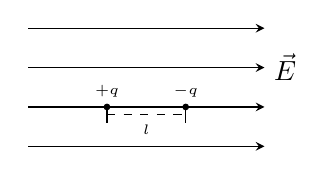
\begin{tikzpicture}
    \foreach \y in {0,0.5,1,1.5}
    \draw [->,>=stealth] (0,\y)--(3,\y); 
    \filldraw  (1,0.5) circle [radius=1pt] node [anchor=south] {\tiny $+q$};
    \filldraw  (2,0.5) circle [radius=1pt] node [anchor=south] {\tiny $-q$};
    \draw (1,0.5)--(1,0.3);
    \draw (2,0.5)--(2,0.3);
    \draw[dashed] (1,0.4)--(2,0.4);
    \draw (1.5,0.4) node [anchor=north]{\tiny $l$};
    \draw (3,1) node [anchor=west] {$\vec{E}$};
  \end{tikzpicture}
  \caption{电偶极子的极化能}
  \label{fig:dianoujizi}
\end{figure}

\begin{gather}
  \intertext{在图\ref{fig:dianoujizi}中所示电偶极子体系的电势能为}
  E_{pp}=q\varphi_+-q\varphi_-=-ql\frac{\varphi_+-\varphi_-}{l}
  \intertext{由电偶极子定义及电场强度计算公式可得上式为}
  E_p=-\vec{p}\cdot\vec{E}
  \intertext{如所考虑的区域存在多个电荷,则其总的能量可以表达为多个电偶极子能量之和,对上式的各电偶极子求和可得电极化强度$\vec{P}=\sum\vec{p}$,所以微小带电体系在静电场中所具有的电势能为}
  E_{pp}=-\vec{P}\cdot\vec{E}
\end{gather}

\subsection{磁化能}

考虑一个磁偶极子,一个矩形微小电流处于磁场中,如图\ref{fig:cioujizi}所示

\begin{figure}[H]
  \centering
  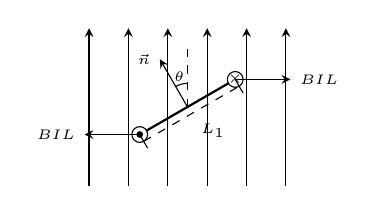
\begin{tikzpicture}
    \foreach \x in {-0.5,0,0.5,1,1.5,2}
    \draw [->,>=stealth] (\x,0)--(\x,2);
    \draw[thick] (0.75,1)++(210:0.6)--++(30:1.2);
    \draw (0.75,1)++(210:0.7) circle [radius=0.1]; 
    \filldraw (0.75,1)++(210:0.7) circle [radius=1pt]; 
    \draw (0.75,1)++(210:0.6)++(30:1.3) circle [radius=0.1];
    \draw (0.75,1)++(210:0.6)++(30:1.3) node {\tiny $\times$};
    \draw[->,>=stealth] (0.75,1)--++(120:0.7) node [anchor=east]{\tiny $\vec{n}$};
    \draw[->,>=stealth] (0.75,1)++(210:0.7)--++(180:0.7) node [anchor=east]{\tiny $BIL$}; 
    \draw[->,>=stealth] (0.75,1)++(210:0.6)++(30:1.3)--++(0:0.7) node [anchor=west]{\tiny $BIL$}; 
    \draw[dashed] (0.75,1)--(0.75,1.8);
    \draw(0.75,1.3) arc (90:120:0.3);
    \draw (0.75,1)++(105:0.4) node {\tiny $\theta$};
    \draw(0.75,1)++(210:0.7)--++(300:0.2);
    \draw(0.75,1)++(30:0.7)--++(300:0.2);
    \draw[dashed](0.75,1)++(210:0.7)++(300:0.1)--++(30:1.4);
    \draw(0.75,1)++(210:0.7)++(300:0.1)++(30:0.7) node [anchor=north west]{\tiny $L_1$};
  \end{tikzpicture}
  \caption{磁偶极子的能量}
  \label{fig:cioujizi}
\end{figure}

\begin{gather}
  \intertext{在图\ref{fig:cioujizi}中,磁偶极子垂直于纸面的宽度为$L$,在纸面上标出的部分长为$L_1$,求出其由图中所示角度转到$\theta=\frac{\pi}{2}$(零磁势能位置)安培力矩做功,则就是此位置时磁偶极子具备的磁化能,即}
  E_{pm}=\int_\theta^{\frac{\pi}{2}} BILL_1\sin\theta d\theta =-\vec{m}\cdot\vec{B}
  \intertext{由于电流分布区域非常小,所以可以视磁场为匀强磁场,同时将电流分解为若干个小环形电流,则求和可得此电流系统所具有的磁化能.磁化强度$\vec{M}=\sum\vec{m}$,所以得微小电流系统在磁场中所具有的磁化能为}
  E_{pm}=-\vec{M}\cdot\vec{B}
\end{gather}
\section{朗德因子}

这一节讨论在于说明统计物理学中关于理想气体磁性的相关公式,同时由于最初学习原子物理时,并没有接受自旋的概念,所以并不是很清楚朗德因子讨论的是什么问题.所以在读朗道的《统计力学》时,决定重新论证一下.

关于自旋,最初的感觉是不能接受,其原因在于平时学习时对于某些概念上理解的不足.但是伴随量子力学和电动力学的学习,我接受了这一概念,肯定这些基本粒子是有内部结构的或者是有自身运动则在以其质心为参考点的系统内,可以肯定其角动量的存在.但是朗道的观点我认为更加合理,当在球坐标系下描述粒子时,不是把粒子当成一个质点,它需要角部的描述,则必然存在一个$l$量子数,所以不必指明是什么来源也可以肯定其角动量的存在,所以自旋即是粒子的内禀角动量,所谓内禀角动量是指以其质心为参考系时,所计算出的角动量.\footnote{《朗道理论物理教程》\quad 卷一\quad 力学( 第5版) $\S 33$ 节.}

考虑到轨道角动量和自旋角动量的耦合,则轨道角动量就是粒子质心的运动所对应的角动量,而自旋是相对于质心坐标系的内禀角动量.但是当计算放在磁场中的带电系统时,其在磁场中的磁化能时所涉及的磁矩与角动量具备一定的关系,但不一定都是线性对应关系.

\begin{figure}[H]
  \centering
  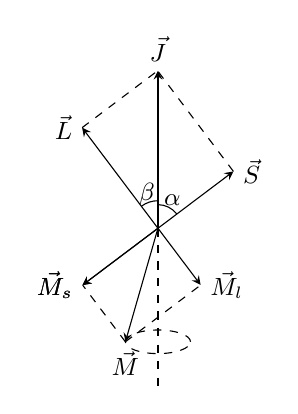
\begin{tikzpicture}
    \draw [->,>=stealth] (0,0)--(0,2) node [anchor=south] {\small $\vec{J}$}; 
    \draw [->,>=stealth] (0,0)--(37:1.2) node [anchor=west] {\small $\vec{S}$};
    \draw [->,>=stealth] (0,0)--(127:1.6) node [anchor=east] {\small $\vec{L}$};
    \draw [dashed] (37:1.2)--++(127:1.6);
    \draw [dashed] (127:1.6)--++(37:1.2);
    \draw [->,>=stealth] (0,0)--(217:1.2) node [anchor=east]{\small $\vec{M}_s$};
    \draw [->,>=stealth] (0,0)--(217:1.2) node [anchor=east]{\small $\vec{M}_s$};
    \draw [->,>=stealth] (0,0)--(307:0.9) node [anchor=west]{\small $\vec{M}_l$};
    \draw [->,>=stealth] (0,0)--(254:1.5) node [anchor=north]{\small $\vec{M}$};
    \draw [dashed] (254:1.5)--++(37:1.2);
    \draw [dashed] (254:1.5)--++(127:0.9);
    \draw [dashed] (0,0)--(0,-2);
    \draw (37:0.3) arc (37:90:0.3);
    \draw (63:0.4) node {\small $\alpha$};
    \draw (90:0.35) arc (90:127:0.35);
    \draw (108:0.45) node {\small $\beta$};
    \draw[dashed] (0,-1.4419) ellipse (0.4135 and 0.15);
  \end{tikzpicture}
  \caption{朗德因子的计算}
  \label{fig:langdeyinzi}
\end{figure}

\begin{gather}
  \intertext{一般情况下根据磁矩 $\vec{M}$ 和角动量$\vec{J}$ 的定义,可得轨道角动量 $\vec{L}$ 和轨道磁矩 $\vec{M}_l$ 的关系}
  \vec{M}_l=\frac{e}{2m}\vec{L}
  \intertext{考虑到量子表达式,则 Bohr 磁子(磁矩的自然单位)为$\mu$ $=$ $\frac{e\hbar}{2m}$, 则上式的标量式为}
  M_l =\mu\sqrt{l(l+1)}
  \intertext{在磁矩和角动量的关系中,质量$m$ 指的是运动粒子的净质量,但是电子的电磁质量和净质量不能明确区分开来,按照电动力学的结论可以取电磁质量和净质量相等,所以测得电子的质量就是这二者之和.因此对于电子内禀角动量自旋而言,则有关系}
  \vec{M}_s=\frac{e}{m}\vec{S}
  \intertext{则上式的标量式为}
  M_s =2\mu\sqrt{s(s+1)}
  \intertext{由于所研究的系统仅在磁场中时所受合外力矩为0,所以总角动量守恒,因此轨道角动量和自旋角动量所构成的平行四边形不变,但是还要绕总角动量方向转动,由于原子是稳定的,所以在所考虑的时间范围内轨道角动量和自旋角动量已经绕总角动量旋转了很多周,则总磁矩在总角动量垂直方向的分量在时间上平均值为零,因此整体上有效的磁矩是沿总角动量方向的分量$M_J$,即}
  \overline{M}=(L_J+2S_J)\frac{e}{2m}
  \label{eq:langde0}
  \intertext{据图\ref{fig:langdeyinzi},设各角动量的大小分别由其对应大写字母表示,对应量子数以其小写字母表示,则由勾股定理可得}
  \vec{L}^2+\vec{J}^2-\vec{S}^2=2\vec{L}\cdot\vec{J}
  \intertext{解得轨道角动量沿总角动量的分量$L_J$ 为}
  L_J=\frac{L^2+J^2-S^2}{2J}
  \intertext{对自旋角动量的沿总角动量的分量 $S_J$,同理可得}
  S_J=\frac{S^2+J^2-L^2}{2J}
  \intertext{代入式\eqref{eq:langde0}得}
  <\vec{M}> =\left\{
    1+\frac{j(j+1)-l(l+1)+s(s+1)}{2j(j+1)}
  \right\}\cdot\frac{e}{2m}\vec{J}
  \intertext{上式的标量式为}
  <M> =\left\{
    1+\frac{j(j+1)-l(l+1)+s(s+1)}{2j(j+1)}
  \right\}\cdot\sqrt{j(j+1)}\mu
  \intertext{记比例系数为$g$,此系数就是朗德因子,即}
  g=1+\frac{j(j+1)-l(l+1)+s(s+1)}{j(j+1)}
  \intertext{则此原子体系放入匀强磁场中的磁势能 $E_{pm}$ 为}
  E_{pm}=-\vec{M}\cdot\vec{B}
  \intertext{选外磁感应强度方向为$z$轴,所以记总角动量在$B$方向的投影为$m_j$,用系统总角动量表达上述磁势能,则}
  E_{pm}=g m_j \cdot \mu B \qquad (m_j=j,j-1,\cdots , -j+1,-j)
\end{gather}

\chapter{经典力学}
\section{Possion 括号}
\begin{align}
  \intertext{这一节主要论述Possion 括号的展开性质,设三个关于广义动量和坐标的函数 A,B,C,同时采用Einsterin 约定对重标求和,则}
  [ [A,B],C]&=
  \left [\frac{\partial A}{\partial p_i}\frac{\partial B}{\partial q_i},C \right]
  -\left [\frac{\partial A}{\partial q_i}\frac{\partial B}{\partial p_i},C \right]\notag\\
  [ [A,B],C]&=
  \left [\frac{\partial A}{\partial p_i}, C \right ]\frac{\partial B}{\partial q_i}-\left [ \frac{\partial A}{\partial q_i},C\right ] \frac{\partial B}{\partial p_i}
  +\frac{\partial A}{\partial p_i}\left [\frac{\partial B}{\partial q_i},C\right ]-\frac{\partial A}{\partial q_i}\left [ \frac{\partial B}{\partial p_i},C\right ]
  \intertext{按微分法则将上式展开,则}
  [ [A,B],C]&=\frac{\partial[A,C]}{\partial p_i}\frac{\partial B}{\partial q_i}-\frac{\partial [A,C]}{\partial q_i}\frac{\partial B}{\partial p_i}
  +\frac{\partial A}{\partial p_i}\frac{\partial [B,C]}{\partial q_i}-\frac{\partial A}{\partial q_i}\frac{\partial [B,C]}{\partial p_i}\notag\\
  &\quad -\left [ A,\frac{\partial C}{\partial p_i}\right ]\frac{\partial B}{\partial q_i}+\left [ A,\frac{\partial C}{\partial q_i}\right ]\frac{\partial B}{\partial p_i}-\frac{\partial A}{\partial p_i}\left [ B,\frac{\partial C}{\partial q_i}\right ]
+\frac{\partial A}{\partial q_i}\left [ B,\frac{\partial C}{\partial p_i}\right ]
\label{eq:possionkh0}
\intertext{式 \eqref{eq:possionkh0}第一行可以用 Possion 括号来表示,则化为}
[ [A,B],C]&=[ [A,C],B]+[A,[B,C]]\notag\\
  &\quad -\left [ A,\frac{\partial C}{\partial p_i}\right ]\frac{\partial B}{\partial q_i}+\left [ A,\frac{\partial C}{\partial q_i}\right ]\frac{\partial B}{\partial p_i}-\frac{\partial A}{\partial p_i}\left [ B,\frac{\partial C}{\partial q_i}\right ]
+\frac{\partial A}{\partial q_i}\left [ B,\frac{\partial C}{\partial p_i}\right ]
\label{eq:possionkh1}
\intertext{式\eqref{eq:possionkh1}中的第二行为零,曾经我试图走一些捷径来论证,但是似乎并不严谨,所以这里我认为具体算出就好,对于第二式中的各项分别计算如下}
-&\left [A,\frac{\partial C}{\partial p_i} \right ]\frac{\partial B}{\partial q_i}=\frac{\partial A}{\partial q_j}\frac{\partial^2 C}{\partial p_i\partial p_j}\frac{\partial B}{\partial q_i}-\frac{\partial A}{\partial p_j}\frac{\partial^2 C}{\partial p_i\partial q_j}\frac{\partial B}{\partial q_i}
\label{eq:possionkh2}\\
 &\left [A,\frac{\partial C}{\partial q_i} \right ]\frac{\partial B}{\partial p_i}=\frac{\partial A}{\partial p_j}\frac{\partial^2 C}{\partial q_i\partial q_j}\frac{\partial B}{\partial p_i}-\frac{\partial A}{\partial q_j}\frac{\partial^2 C}{\partial q_i\partial p_j}\frac{\partial B}{\partial p_i}
\label{eq:possionkh3}\\
-&\frac{\partial A}{\partial p_i}\left [B,\frac{\partial C}{\partial q_i} \right ]=\frac{\partial A}{\partial p_i}\frac{\partial^2 C}{\partial q_i\partial p_j}\frac{\partial B}{\partial q_j}-\frac{\partial A}{\partial p_i}\frac{\partial^2 C}{\partial q_i\partial q_j}\frac{\partial B}{\partial p_j}
\label{eq:possionkh4}\\
&\frac{\partial A}{\partial q_i}\left [B,\frac{\partial C}{\partial p_i} \right ]=\frac{\partial A}{\partial q_i}\frac{\partial^2 C}{\partial p_i\partial q_j}\frac{\partial B}{\partial p_j}-\frac{\partial A}{\partial q_i}\frac{\partial^2 C}{\partial p_i\partial p_j}\frac{\partial B}{\partial q_i}
\label{eq:possionkh5}
\intertext{由于 $i,j$ 是求和的下标号,它们是独立的,所以交换它们并不改变和式的值, 同时对函数取二重偏微分时对不同自变量的微分顺序微分值也是相同的.考虑到这一点,则 \eqref{eq:possionkh2} + \eqref{eq:possionkh3} + \eqref{eq:possionkh4} + \eqref{eq:possionkh5} = 0 ,则式 \eqref{eq:possionkh1}化为}
&[ [A,B],C]=[ [C,B],A]+[ [A,C],B]
\label{eq:possionkh6}
\intertext{上式的写法规则是:左式等于交换 $A,C$ 与 交换 $B,C$ 的和.此式也可以写成轮换式,即}
&[ [A,B],C]+[ [B,C], A]+ [ [C,A],B]=0
\label{eq:possionkh7}
\end{align}


\chapter{非理想气体}

\section{范德瓦尔斯公式}
第208页,习题4.对于范德瓦尔斯气体,求焦耳---汤姆孙过程反转点对温度的依赖关系.在书中没有具体写出计算过程,此处就是这个过程.范德瓦尔斯气体方程为

\begin{equation}
  \left(p+\frac{N^2a}{V^2}\right)\left(V-Nb\right)=NT
  \label{eq:VanderWaals}
\end{equation}

\vspace{-30pt}
\begin{gather}
  \intertext{反转曲线由$\left(\frac{\partial T}{\partial p}\right)_H=0$决定,则}
  \difh H = T\diff S +V \diff p =
  T\left(\frac{\partial S}{\partial T}\right)_p \diff T 
  +\left[T \left(\frac{\partial S}{\partial p}\right)_T+V\right]\diff p=0
  \intertext{解得}
  \left(\frac{\partial T}{\partial p}\right)_H
  =-\frac{1}{T\left(\frac{\partial S}{\partial T}\right)_p}\cdot 
  \left[T \left(\frac{\partial S}{\partial p}\right)_T+V\right]
  \intertext{由定压热容量和麦克斯韦关系将上式化为}
  \left(\frac{\partial T}{\partial p}\right)_H
  =\frac{1}{C_p}\left[T\left(\frac{\partial V}{\partial T}\right)_p-V\right]
  \intertext{于是得反转曲线}
  \left(\frac{\partial T}{\partial V}\right)_p =\frac{T}{V}
  \label{eq:VanderWaals0}
  \intertext{将式\eqref{eq:VanderWaals}代入式\eqref{eq:VanderWaals0}得反转曲线}
  T\cdot\frac{N}{V}=-2a\frac{N^2}{V^3}\left(V-Nb\right)+\left(p+a\frac{N^2}{V^2}\right) 
  \label{eq:VanderWaals1}
  \intertext{记粒子数密度$n=\frac{N}{V}$,则式\eqref{eq:VanderWaals}和式\eqref{eq:VanderWaals1}可以写成}
  \left\{
    \begin{gathered}
      (p+an^2)(1-bn)=Tn\\
      p-an^2+2abn^3=Tn
    \end{gathered}
  \right.
  \label{eq:VanderWaals2}
  \intertext{令上述二式相等,约去$Tn$得}
  3ab\cdot n^2-2a\cdot n+pb=0
  \label{eq:VanderWaals3}
  \intertext{解得}
  n=\frac{1\pm \sqrt{1-\frac{3b^2}{a}p}}{3b}
  \label{eq:VanderWaals4}
  \intertext{由式\eqref{eq:VanderWaals3}可得}
  p+an^2=\frac{2a}{b}(1-bn)
  \label{eq:VanderWaals5}
  \intertext{式\eqref{eq:VanderWaals5}代入式\eqref{eq:VanderWaals2}可得}
  T=\frac{2a}{b}(1-nb)^2
  \label{eq:VanderWaals6}
  \intertext{式\eqref{eq:VanderWaals4}代入式\eqref{eq:VanderWaals6}得}
  T=\frac{2a}{9b}\left(2\mp \sqrt{1-\frac{3b^2}{a}p}\right)^2
\end{gather}

\section{位力系数与散射振幅的关系}

原文中计算的是对动量$p$的微分,但是考虑到 德布罗意关系$p=\hbar k$我在这时修改为对$k$的微分,这样在式中不会出现$\hbar$,单纯的讨论数学计算而己.
\begin{equation}
  \sum_{l=0}^\infty (2l+1)\cdot \frac{\mathrm{d}\delta_l}{\mathrm{d}k}
  =\frac{\partial}{\partial k} \frac{k}{2}\left[f(0)+f^*(0)\right]
  +\frac{1}{4\pi i}\int k^2(f^*\frac{\partial f}{\partial k}-f\frac{\partial f^*}{\partial k})\mathrm{d}\Omega
  \label{eq:zhenfu}
\end{equation}

{\bf 证明} 量子力学中已经计算出了散射振幅如下\footnote{这些计算我在我自己的笔记《特殊函数基础》中所做的,这里为了完整而直接引用.} 

\begin{gather}
  f(\theta)=\frac{1}{k}\sum_{l=0}^\infty (2l+1)P_l(\cos\theta)e^{i\delta_l}\cdot \sin\delta_l
  \label{eq:zhenfu0}
  \intertext{考虑到$P_l(1)=1$,则式\eqref{eq:zhenfu0}中$\theta=0$得}
  kf(0)=\sum_{l=0}^\infty (2l+1)e^{i\delta_l}\cdot \sin\delta_l
  \label{eq:zhenfu1}
  \intertext{上式对 $k$ 微分,得}
  \frac{\partial kf(0)}{\partial k}=\sum_{l=0}^{\infty} \cdot e^{i2\delta_l}\cdot \frac{\mathrm{d}\delta_l}{\mathrm{d}k}
  \label{eq:zhenfu2}
  \intertext{对式\eqref{eq:zhenfu2}求共轭,得}
  \frac{\partial kf^*(0)}{\partial k}=\sum_{l=0}^{\infty} \cdot e^{-i2\delta_l}\cdot \frac{\mathrm{d}\delta_l}{\mathrm{d}k}
  \label{eq:zhenfu3}
  \intertext{\eqref{eq:zhenfu2}+\eqref{eq:zhenfu3}再除以2得}
  \frac{\partial}{\partial k}\frac{k}{2}\left[f(0)+f^*(0)\right]
  =\sum_{l=0}^\infty(2l+1)\cos2\delta_l \cdot \frac{\mathrm{d}\delta_l}{\mathrm{d}k}
  \label{eq:zhenfu4}
  \intertext{如$\theta$ 没有取零,则}
  \frac{\partial kf}{\partial k}=\sum_{l=0}^{\infty} \cdot e^{i2\delta_l}\cdot P_l(\cos\theta)\cdot \frac{\mathrm{d}\delta_l}{\mathrm{d}k}
  \label{eq:zhenfu5}
  \intertext{同时将式\eqref{eq:zhenfu0}左右同乘以$k$ 再取共轭得}
  kf^*(\theta)=\sum_{l=0}^\infty (2l+1)P_l(\cos\theta)e^{-i\delta_l}\cdot \sin\delta_l
  \label{eq:zhenfu6}
  \intertext{式\eqref{eq:zhenfu5}乘以式\eqref{eq:zhenfu6}再对立体角求积分以消去$P_l(\cos\theta)$计算结果为}
  \int kf^*\frac{\partial kf}{\partial k}\mathrm{d}\Omega =4\pi \sum_{l=0}^\infty (2l+1)\cdot e^{i\delta_l}\cdot \sin\delta_l \cdot \frac{\mathrm{d}\delta_l}{\mathrm{d}k}
  \label{eq:zhenfu7}
  \intertext{对式\eqref{eq:zhenfu7}求共轭,得}
  \int kf\frac{\partial kf^*}{\partial k}\mathrm{d}\Omega =4\pi \sum_{l=0}^\infty (2l+1)\cdot e^{-i\delta_l}\cdot \sin\delta_l \cdot \frac{\mathrm{d}\delta_l}{\mathrm{d}k}
  \label{eq:zhenfu8}
  \intertext{式\eqref{eq:zhenfu7}加上式\eqref{eq:zhenfu8}可以得}
  \int \left(kf^*\frac{\partial kf}{\partial k}-kf\frac{\partial kf^*}{\partial k}\right)\mathrm{d}\Omega
  =8\pi i\sum_{l=0}^\infty (2l+1)\cdot \sin^2\delta_l \cdot\frac{\mathrm{d}\delta_l}{\mathrm{d}k}
  \label{eq:zhenfu9}
  \intertext{由三角函数半角公式可得式\eqref{eq:zhenfu9}化为}
  \frac{1}{4\pi i}\int \left(kf^*\frac{\partial kf}{\partial k}-kf\frac{\partial kf^*}{\partial k}\right)\mathrm{d}\Omega
  =\sum_{l=0}^\infty (2l+1)\cdot (1-\cos2\delta_l) \cdot\frac{\mathrm{d}\delta_l}{\mathrm{d}k}
  \label{eq:zhenfu10}
  \intertext{式\eqref{eq:zhenfu9}和式\eqref{eq:zhenfu10}相加消去$\cos2\delta_l$便得到式\eqref{eq:zhenfu}}
  \sum_{l=0}^\infty (2l+1)\cdot \frac{\mathrm{d}\delta_l}{\mathrm{d}k}
  =\frac{\partial}{\partial k} \frac{k}{2}\left[f(0)+f^*(0)\right]
  +\frac{1}{4\pi i}\int k^2(f^*\frac{\partial f}{\partial k}-f\frac{\partial f^*}{\partial k})\mathrm{d}\Omega
\end{gather}

在上述证明中,其关键点在于消去角度 $\theta$ ,对于振幅的表达式\eqref{eq:zhenfu0}而言我们总共有两种方法达成这个目的.其一,令$\theta$ 取特殊值,在证明中取了$\theta=0$; 其二,借助积分和 $P_l(\cos\theta)$ 正交性.同时再考虑三角函数的运算,才可以完成和式\eqref{eq:zhenfu}的证明,这是一个相当巧合的技巧.


\chapter{溶液}

\section{强电解质溶液}

强电解质指溶解到溶液中时能够完全电离成离子的物质.其热力学势为
\begin{gather}
  \Phi=N\mu_0+
  \sum_a\left(Tn_a\ln \frac{n_a}{eN}+n_a\Psi_a\right)
  -\frac{2e^3}{3\varepsilon^{\frac{3}{2}}}\cdot
  \left(\frac{\pi}{\nu T}\right)^{\frac{1}{2}}\cdot N
  \cdot \left( \frac{\sum_a n_aZ_a^2}{N}\right)^{\frac{3}{2}}
  \intertext{可以求得一个离子的化学势为}
  \mu_a=\frac{\partial \Phi}{\partial n_a}
  =T\ln\frac{n_a}{eN}+\Psi_a
  -\frac{e^3}{\varepsilon^{\frac{3}{2}}}\cdot
  \left(\frac{\pi}{N\nu T}\right)^{\frac{1}{2}}Z_a
  \cdot \left( \sum_a n_aZ_a^2\right)^{\frac{1}{2}}
\end{gather}
习题:试求加入一定量的第二种电解质(其所有离子与第一种的全都不同)后第一种强电角质溶解度(假设很小)的改变.

{\bf 解:}电解质溶解度的定义为:第a种分子在溶液中最大的浓度.设一个电解质分子所带第a种离子的数量为$\nu_a$,即
\begin{gather}
  c_0=\frac{n_a}{N\nu_a} 
  \intertext{当固体电解质与溶液达到平衡时,其浓度达到最大,就是其溶解度.记$\mu_s$  为电解质分子的化学势,则}
  \mu_s(P,T)=\sum_a \nu_a \mu_a
  \intertext{由于平衡,所以固体中$\mu_a$ 可以使用饱和溶液中的化学势来代入,得}
  \mu_s =T\sum_a \nu_a\ln\frac{n_a}{N}
  +\sum_a \nu_a\mu_a
  -\frac{e^3}{\varepsilon^{\frac{3}{2}}}\cdot
  \left(\frac{\pi}{N\nu T}\right)^{\frac{1}{2}}\cdot
\sum_a\nu_aZ_a^2\cdot
\left( \sum_b n_bZ_b^2\right)^{\frac{1}{2}}
\intertext{在上式中对a的求和,是和固态电解质平衡的成份,也就是它们的浓度就是溶解度.但是对b的求和,包含了溶液中的全部溶质成份.当再加入另一种电解质后,则已达饱和的a类离子将不发生变化,而新加入的离子就在对b求和的和式中,这在推导过程中很清楚.所以对第a种离子的溶解度的影响,是由对b的和式导致的,由于平衡时热力学势取极小值,因此对其变分就可以得到溶解度的影响.即}
T\sum_a \nu_a \cdot \frac{\delta c_0}{c_0}
-\frac{e^3}{\varepsilon^{\frac{3}{2}}}
\left(\frac{\pi}{N\nu T}\right)^{\frac{1}{2}}\cdot
\sum_a\nu_a Z_a^2 \cdot \frac{1}{\sqrt{\sum_an_aZ_a^2}}\cdot 
\delta \left(\sum_an_aZ_a^2\right)=0
\intertext{简单整理可得}
\delta c_0=\frac{e^3\pi^{\frac{1}{2}}}{2v^\frac{1}{2}(T\varepsilon N)^{\frac{3}{2}}\sum_a\nu_a}
\cdot \left(\sum_bn_bZ_b^2\right)^{\frac{1}{2}}\cdot
\delta \left(\sum_bn_bZ_b^2\right)
\end{gather}
变分号后的和式只含另加的离子类型,因为它是由于新加入的离子导致的变化.在所考虑的条件溶解度增加.

\chapter{化学反应}

\section{化学平衡条件}

在朗道书第267页,第三段中列举了化学反应
\begin{equation}
  2H_2+O_2=2H_2O
  \label{eq:HOfanying}
\end{equation}
在将其写成热力学表达式时,朗道书中写的是
\begin{equation}
  2H_2+O_2-2H_2O=0
\end{equation}
由于每一个化学反应都可以在正逆两个方向发生,所以朗道的这个写法按规定就是水的分解,其中$H_2$和$O_2$是作为生成物写出的.但是在汪志诚《热力学和统计物理学》中 \S 4.5 化学平衡条件 一节中写成了式
\begin{equation}
  2H_2O-2H_2-O_2=0
\end{equation}
此式写的是$H_2$ 和 $O_2$ 的化合反应.我最初的教材是汪志诚的书,由于这两个不同的写法,导致我在2019年6月30号计算朗道书第270页习题1时,出现了困难,我的计算结果不能与朗道书中的结果对应起来,这个麻烦是在7月1号上班后,仔细对比后确定出了两本书的不同.

\chapter{涨落}
\newcommand{\fangjunzhi}[1]{\left<#1^2\right>}
\section{高斯分布}
高斯分布指如下形式的分布
\begin{gather}
  \omega(x)dx=Ae^{-\frac{\beta}{2}x^2}dx
  \intertext{对上式$x$从$-\infty$ 到$\infty$据归一化可得系数$A$,即}
  A\sqrt{\frac{2\pi}{\beta}}=1
  \intertext{解得}
  A=\sqrt{\frac{\beta}{2\pi}}
  \intertext{所以高斯分布为}
  \omega(x)=\sqrt{\frac{\beta}{2\pi}}e^{-\frac{\beta}{2}x^2}
\end{gather}

下面求涨落的方均值即
\begin{gather}
  \left<x^2\right>=\sqrt{\frac{\beta}{2\pi}}\int_{-\infty}^\infty e^{-\frac{\beta}{2}x^2}x^2 dx\notag
  \intertext{上式可以借用偏微分方便的计算为}
  \left<x^2\right>=-2\sqrt{\frac{\beta}{2\pi}}\frac{\partial}{\partial \beta}
  \int_{-\infty}^\infty e^{-\frac{\beta}{2}x^2} dx
  \intertext{上式积分容易算出,得}
  \left<x^2\right>=-2\sqrt{\frac{\beta}{2\pi}}\frac{\partial}{\partial \beta}
  \sqrt{\frac{2\pi}{\beta}}
  \intertext{稍加整理得}
  \left<x^2\right>=\frac{1}{\beta}
\end{gather}

将高斯分布中的$\beta$用方均值代替,则高斯分布又可以表达为
\begin{equation}
  \omega(x)=\frac{1}{\sqrt{2\pi\fangjunzhi{x}}}e^{-\frac{x^2}{2\fangjunzhi{x}}}
  \label{eq:gaussfenbu}
\end{equation}

\section{多个热力学量的高斯分布}

由于孤立系统的熵在达到平衡时具有极大值,所以在平衡位置,可以将熵 Taylor 展开,而保留到二级项,因为一级微分项为零.同时,基于极大值的考虑,则二级项应当是负定二次型,为了方便表述采用了Einstein 约定,对重复的下标默认表示从$1$ 到$n$ 求和,即
\begin{gather}
  S-S_0 = -\frac{1}{2}\beta_{ij}x_ix_j 
  \intertext{二阶张量是对称的,即$\beta_{ij}=\beta_{ji}$,所以多个热力学量的分布也构成高斯分布}
  \omega(x_1,x_2,\cdots ,x_n)=Ae^{-\frac{1}{2}\beta_{ij}x_ix_j}
  \label{eq:multigauss0}
  \intertext{系数$A$ 同样可以据归一化来求出,但是直接求解不是很好处理.所以此处先把二次型写成标准型,设变换矩阵为$a_{ij}$,则}
  \beta_{ij}x_ix_j=\beta_{ij}a_{il}a_{jk}x_l'x_k'
  \label{eq:multigauss1}
  \intertext{在式\eqref{eq:multigauss1}中令系数为$\delta_{lk}$则二次型化为标准型,即}
  \beta_{ij}a_{il}a_{jk}=\delta_{lk}
  \label{eq:multigauss2}
  \intertext{式\eqref{eq:multigauss2}一共有$n^2$组等式,同时含有$n^2$个未知数,所以它有唯一解,同时$a_{ij}=a_{ji}$,即变换矩阵为对称矩阵.同时由Jacobi 行列式可以得到微元变换为}
  \frac{\partial(x_1,x_2,\cdots,x_n)}{\partial(x_1',x_2',\cdots,x_n')}
=\left|a_{ij}\right|=a
\intertext{对\eqref{eq:multigauss0}关于$n$个变量积分,得}
A\int \cdots \int e^{-\frac{1}{2}\beta_{ij}x_ix_j}\mathrm{d}{x_1}\mathrm{d}{x_2}\cdots\mathrm{d}{x_n}
=
Aa\int \cdots \int e^{-\frac{1}{2}x_i'x_i'}\mathrm{d}{x'_1}\mathrm{d}{x'_2}\cdots\mathrm{d}{x'_n}=Aa(2\pi)^{\frac{n}{2}}=1
\intertext{解得系数为}
A=\frac{1}{a(2\pi)^{\frac{n}{2}}}
\end{gather}

在前述的变换矩阵$|a_{ij}|$,我们是不需要直接求解出来的,因为本身高斯分布已经完全确定了分布,所以在各平均值的计算结果中是不会出现变换矩阵的有关信息的.记热力学共轭量为$X_i$,则按定义其为
\begin{equation}
  X_i=-\frac{\partial S}{\partial x_i}=\beta_{il}x_l
  \label{eq:hotgonger}
\end{equation}
这里主要计算的涨落信息是$\left<x_ix_j\right>$ 和$\left<X_iX_j\right>$,这里有两种算法,其一是按朗道的计算方法,此法相当简洁明了;其二直接计算就好.

\subsubsection{朗道的计算方法}
令$\overline{x_i}=x_{0i}$则高斯分布可以写为
\begin{gather}
  \omega(x_1,x_2,\cdots ,x_n)=\frac{1}{a(2\pi)^{\frac{n}{2}}}e^{-\frac{1}{2}\beta_{ij}(x_i-x_{0i})(x_j-x_{0j})}
  \intertext{可以计算均值如下}
 \int \frac{1}{a(2\pi)^{\frac{n}{2}}}e^{-\frac{1}{2}\beta_{ij}(x_i-x_{0i})(x_j-x_{0j})}
 x_l \mathrm{d}x_1\mathrm{d}x_2\cdots\mathrm{d}x_n=x_{0l}
 \intertext{对$x_{0k}$微分,则右式为$\delta_{lk}$上式 即}
 \int \frac{1}{a(2\pi)^{\frac{n}{2}}}e^{-\frac{1}{2}\beta_{ij}(x_i-x_{0i})(x_j-x_{0j})}
 x_lX_k \mathrm{d}x_1\mathrm{d}x_2\cdots\mathrm{d}x_n=x_{0l}
 \intertext{上式可以简写如下}
 \left<x_lX_k\right>=\delta_{lk}
 \intertext{上式的共轭量用$x_i$展开,则}
 \beta_{ki}\left<x_ix_l\right>=\delta_{lk}
 \intertext{记矩阵$\beta_{ki}$的逆为$\beta^{-1}_{ki}${\bf 注意不是倒数},由此式可得}
 \left<x_ix_l\right>=\beta^{-1}_{il}
 \intertext{同时也可以求得共轭量的乘积平均值}
 \left<X_iX_l\right>=\beta_{ik}\left<x_kX_l\right>=\beta_{ik}\delta_{kl}
 \intertext{即}
 \left<X_iX_l\right>=\beta_{il}
\end{gather}

\subsubsection{直接计算法}

\begin{align}
  \left<x_ix_j\right>&=A\int x_ix_je^{-\frac{1}{2}\beta_{lm}x_lx_m} 
  \mathrm{d}x_1 \mathrm{d}x_2\cdots\mathrm{d}x_n\notag\\
  &=a_{ik}a_{jm}Aa\int x'_kx'_m e^{-\frac{1}{2}x'_lx'_l}
  \mathrm{d}x'_1 \mathrm{d}x'_2\cdots\mathrm{d}x'_n\notag\\
  &=a_{ik}a_{jm}\delta_{km}\notag\\
  &=a_{ik}a_{jk}=a_{ik}a_{kj}
  \label{eq:xixj0}
\end{align}
同时由于
\begin{gather}
  \beta_{ij}a_{ik}a_{jl}=\delta_{kl}
  \intertext{所以}
  \beta_{ij}a_{ik}a_{kj}=1
  \intertext{于是可得$a_{ik}a_{kj}$为}
  a_{ik}a_{kj}=\beta_{ij}^{-1}
  \intertext{上式代入式\eqref{eq:xixj0}得}
  \left<x_ix_j\right>=\beta_{ij}^{-1}
\end{gather}
下面计算$\left<X_iX_j\right>$,如下
\begin{align}
  \left<X_iX_j\right>&=\beta_{il}\beta_{jk}\left<x_lx_k\right>\notag\\
  &=\beta_{il}\beta_{jk}\cdot \beta_{lk}^{-1}\notag\\
  &=\beta_{il}\cdot \delta_{lj}\notag\\
  &=\beta_{ij}
  \label{eq:XiXj0}
\end{align}

对于多个热力学量的高斯分布,上面的计算技巧为使用线性变换将负定二次型转换为标准型,然后积分就容易进行.同时根据标准型的要求,可得各涨落量使用相应系数的表达.由于这些表达,则容易判断是否统计独立.

\subsubsection{统计独立性的判断}

对于任意两个物理量的平均值,可以先将其它的物理量积分(此积分不会对平均值起作用),然后再求解,即
\begin{gather}
  \left<x_1x_2\right>=A\int e^{-\frac{1}{2}\beta_{11}'x_1^2-\beta_{12}'x_1x_2-\frac{1}{2}\beta_{22}'x_2^2} x_1x_2\mathrm{d}x_1\mathrm{d}x_2 
  \intertext{由此可得}
  \left<x_1x_2\right>=\beta_{12}^{\prime -1}
  \intertext{同理}
  \left<X_1X_2\right>=\beta_{12}'
  \intertext{为了讨论方便省去右上角的$\prime$号,则由行列式的代数余子式可以构成矩阵的逆,对于二阶矩阵可得其逆为}
  \beta_{12}^{-1}=\frac{\beta_{12}}{\beta_{12}^2-\beta_{11}\beta_{22}}
\end{gather}
上式表明了,如果$\beta_{12}^{-1}=0$,则$\beta_{12}=0$,也就是说如果$\left<x_1x_2\right>=0$,则$\left<X_1X_2\right>=0$.即\CJKunderwave{如果某热力学量统计独立,则和该物理量对应的共轭量也统计独立.}

\chapter{二次量子化}
今天是2019年7月13日,暑假正式开始.在学习统计物理学中的第十二章 {\bf \S 117 简并气体中的密度涨落关联 }时用到了量子力学中的二次量子化方法,但是作为考研的准备,对于二次量子化并没有太多的研究,同时理解起来有一定的难度,但是作为学习之用我感觉到了二次量子化的重要性,所以集中几天的时间学习理解二次量子化.学习的基础是朗道《量子力学(非相对论)》,由于长时间没有集中精力学习量子力学所以导致最近几天十分头疼,理解之后记录这一章的核心内容.\footnote{这一章对应量子力学{\bf 第九章 粒子的全同性}}

\section{同类粒子的不可分辨原理}

微观领域物体的运动是遵守量子力学规律的.比如两个电子,如果它们服从经典力学,则我们可以分辨它们.方法是记录它们开始运动的位置,然后按按照刘维定理,每个粒子都有确定的轨道,所以分辨出轨道就分辨出电子了.但是实际情况不是这样,比如在某一时刻,我们确定的电子的位置,但是在任意小的任意时刻我们不能给出电子的确切位置,所以根本无法按照经典力学定义速度!因为经典速度指当$\Delta t$ 趋近零时,位移与时间的比值,但是这里既然位移无法给出,则速度也就无从谈起,所以也不会有轨道了.因此在量子力学的意义上,我们即使开始给粒子编了号,但是在任意小的一段时间内,我们无法说明到底是检测到了哪一个粒子.在量子力学的层面上我们谈论的问题就变成了在哪个位置发现了几个电子,且能够发现几个电子的概率是多少.


由于同类粒子的不可分辨原理,我们在描述粒子的时候只能写出这些粒子所满足的量子力学方程,并确定它们所遵守的波函数.但是根据Schr\"odinger 方程所确定的波函数,还有一个不会影响相对概率分布的相角,这一点需要注意.由于粒子不可分辨,所以在交换粒子时波函数将会发生一些变化,交换粒子意味着对换波函数中两个粒子的所有坐标.而粒子又是不可分辩的,所以交换任意两个全同粒子的坐标后,波函数的变化是不会导致相对概率的变化的,也就是最多出现一个相因子,即
\begin{gather}
  \Psi(\xi_1,\xi_2)=e^{i\alpha}\Psi(\xi_2,\xi_1)
  \intertext{再对换一次粒子,则波函数必然变回原来的样子,即}
  \Psi(\xi_1,\xi_2)=e^{i2\alpha}\Psi(\xi_1,\xi_2)
  \intertext{基于波函数的任意性,所以必然有}
  e^{i2\alpha}=1
  \intertext{解得}
  e^{i\alpha}=\pm 1
  \intertext{所以对于波函数就有两种情况}
  \Psi(\xi_1,\xi_2)=\pm\Psi(\xi_2,\xi_1)
\end{gather}
对于交换粒子后波函数取正的情况,我们称满足这个情况的粒子为Bose 子,对于交换粒子后波函数改变一个负号的情况,我们称满足这个情况的粒子为Fermi 子.

根据不同类型的粒子我们可以先从Schr\"odinger 方程解出任意一个解,然后再构造出满足交换规律的波函数.首先,我们从某一个满足Schr\"odinger 方程的函数出发,构造满足对称性的N个Bose 子的波函数形式.记量子态分别为$p_1,p_2,\cdots $ ,同时各粒子用不同的坐标$\xi_1,\xi_2,\cdots $ 来表示,如果两个粒子处于相同的状态,则$p$值相同,但是它们的坐标仍然是已经标定的标号.所以要满足每一对粒子交换都是对称的,则可以如下构造
\begin{gather}
  \Psi = \Sigma \Psi_{p_1}(\xi_1)\Psi_{p_2}(\xi_2)\cdots\Psi_{p_N}(\xi_N) 
\end{gather}
上式中$\Sigma$ 表示对于所有可能的交换求和,在上式中可以理解各$p_i$不动,交换各个坐标$\xi_i$,也可以理解为各 $\xi_i$ 不动,改变各$p_i$,其数学结果是一样的,可以验证我们对于$\Psi$ 而言交换任意两个粒子,其波函数都是对称的.

在上式中所构造的波函数并没有归一化.因为有可能粒子处于同一个状态,比如有$N_1$个粒子处于$\Psi_{p_1}$态,这是有可能的.因为对于处于同一状态的粒子的交换不能产生新的态,所以在各种交换中会出现相同的态,那么各种求和的可能性中总共有项数
\begin{gather}
  \frac{N!}{N_1!N_2!\cdots N_m!} 
\end{gather}
所以得归一化的波函数为
\begin{gather}
  \Psi =\sqrt{\frac{N_1!N_2!\cdots N_m!}{N!}} \Sigma \Psi_{p_1}(\xi_1)\Psi_{p_2}(\xi_2)\cdots\Psi_{p_N}(\xi_N) 
\end{gather}
此时上面的求和应当理解为对所有粒子交换再求和,因为相同的态下粒子的交换,已经由$N_i!$ 而除去了.在上面的下标中,应当理解为$p_1=p_2=\cdots =p_{N_1}$,$p_{N_1}=p_{N_1+1}=\cdots =p_{N_1+N_2}$ ,$\cdots \cdots$.

对于Fermi 子,我们可以构造成如下波函数
\begin{equation}
  \Psi=\frac{1}{\sqrt{N!}}
  \begin{vmatrix}
    \Psi_{p_1}(\xi_1)&\Psi_{p_1}(\xi_2)&\cdots&\Psi_{p_1}(\xi_N)\\
    \Psi_{p_2}(\xi_1)&\Psi_{p_2}(\xi_2)&\cdots&\Psi_{p_2}(\xi_N)\\
    &&\vdots &\\
    \Psi_{p_N}(\xi_1)&\Psi_{p_N}(\xi_2)&\cdots&\Psi_{p_N}(\xi_N)
  \end{vmatrix}
\end{equation}
很显然,在式中交换任意两列或者两行,则波函数都会改变一个负号.同时,不可能有两行是相同的,即$p_i\neq p_j, i\neq j$,如果有两行相同,则行列式为零,此即 泡利不相容原理---同一时刻不可能有两个相同的费米子处于相同的态.

\section{交换作用}

在没有磁场的情况下解Schr\"odinger 方程,我们会得到一系列的解和能级.由于在这种情况下能级中不含自旋,所以导致它不能完全反映波函数的对称性.也就是说,波函数的对称性会对这些解中的一些波函数给出限制,有一些在某种情况下将是不允许的.在这种情况下,波函数可以写成坐标函数和自旋函数的乘积,即
\begin{equation}
  \Psi(\xi_1,\xi_2,\cdots,\xi_n)=\varphi(r_1,r_2,\cdots ,r_N)\cdot X(\sigma_1,\sigma_2,\cdots ,\sigma_n)
\end{equation}
当考虑的是玻色子的时候,要求$\Psi(\xi_1,\xi_2,\cdots ,\xi_N)$为对称波函数,所求的坐标波函数$\varphi(r_1,r_2,\cdots,r_N)$ 如果为对称的,则自旋波函数$X(\sigma_1,\sigma_2,\cdots ,\sigma_n)$ 也是对称的,反之都是反对称的.当所考虑的是费米子时,要求$\Psi(\xi_1,\xi_2,\cdots ,\xi_N)$为反对称波函数,如果坐标波函数$\varphi(r_1,r_2,\cdots,r_N)$ 如果为对称的,则自旋波函数$X(\sigma_1,\sigma_2,\cdots ,\sigma_n)$ 是反对称的,反之则坐标波函反对称,自旋波函对称.但是如果不去考虑这个对称性,则仅有坐标部分求得的波函数和能级就要比考虑了对称性时要多,于是考虑交换对称性会影响到实际的波函和能级.

多电子系统的那些能量允许的值依懒于该系统的总自旋.由于这个原因,我们可以把这种依懒关系说成是粒子间的一种特殊作用的结果.这种作用称为``{\bf 交换作用}''.\footnote{引用自《量子力学(非相对论)》第213页.}

一个自旋为$s$ 的粒子A,它在$z$ 轴方向的投影有$2s+1$个.如果考虑一个复合粒子B,它由$2s$个自旋为$\frac{1}{2}$ 的基本粒子构成,由角动量的合成规则可得,这个复合粒子的最大角动量为$s$,从物理上讲,一个自旋为$s$粒子和这里所述的复合粒子是等价的,从描述方法上来说,不会有什么不同.对于这个复合粒子,它可以由一个$2s$秩旋量来描述,即
\begin{equation}
  X^{\overbrace{\alpha\beta\cdots}^{\text{共2s项}}}
\end{equation}
当粒子A在$z$轴上的分量为$\sigma$ 时,此分量对应如下B的分量
\begin{equation}
  X^{\overbrace{11\cdots}^{s +\sigma}\overbrace{22\cdots}^{s -\sigma}}
\end{equation}
显然B的旋量所表示的自旋在$z$轴上的分量值为$\frac{1}{2}(s+\sigma)-\frac{1}{2}(s-\sigma)=\sigma$,所以分量上来讲也是对应的.复合粒子由$2s$个自旋为$\frac{1}{2}$的全同粒子构成,所以在上述表达式上,哪些粒子取$1$,哪些粒子取$2$,这是不确定的.这就产生以确定具体对应关系的问题,记A的此分量为$\Psi(\sigma)$,则考虑下式成立
\begin{equation}
  \sum_{\sigma=-s}^{s} |\Psi(\sigma)|^2 =\sum_{\alpha\beta\cdots =1}^2 |X^{\alpha\beta\cdots}|^2
\end{equation}
上式确定了在空间一点粒子出现的概率,因为它考虑到了各个自旋的概率出现的和.显然,右式中出现$\sigma$ 的项共有$\frac{(2s)!}{(s+\sigma)!(s-\sigma)!}$ 项,同时又考虑到$s$的任意性,所以可以确定具体对应系为
\begin{equation}
  \Psi(\sigma)=
  \sqrt{\frac{(2s)!}{(s+\sigma)!(s-\sigma)!}}
    X^{\overbrace{11\cdots}^{s+\sigma}\overbrace{22\cdots}^{s-\sigma}}
\end{equation}
需要说明的是在上式中旋量,我们取出了一个任意的分量,将其中所有$1$并到一块,所有的$2$ 并到了一块,当$\sigma$ 增加$1$ 时,在$1$这一分组追加一个,同时在$2$分组减少一个就好.同时在计算项数的数目时,当$s$主半整数时,$s\pm \sigma$也是整数,所以在讨论问题的过程中是兼顾了半整数的.

下面考虑第213页的所述的双粒子系统,每个粒子的自旋为$s$,则需要一个$4s$秩的旋量来描述.即
\begin{equation}
  X^{\overbrace{\nu\mu\cdots}^{2s}\overbrace{\rho\sigma\cdots}^{2s}}
\end{equation}
这两个粒子所能构成的系统的总自旋为$0$,$1$,$2$,$\cdots$,$2s$,当总自旋为$S$,相当于将上述自旋缩并掉$2s-S$个指标,而变成一个$2S$秩旋量,其自旋就是$S$.缩并意味着,可以通过将后$2s-S$个指标移到下标上来,按Einstein 约定,哑标求和.即
\begin{equation}
  X^{\overbrace{\nu\mu\cdots}^{S}\overbrace{\rho\sigma\cdots}^{S}
  \overbrace{\rho'\sigma'\cdots}^{2s-S}}\ _{\underbrace{\rho'\sigma'\cdots}_{2s-S}}
\end{equation}
当交换所有粒子时相当于交换$\nu$,$\mu$,$\cdots$,$\nu'$,$\mu'$,$\cdots$ 和$\rho$,$\sigma$,$\cdots$,$\rho'$,$\sigma'$,$\cdots$ 两组指标.当交换上标和下标时,旋量会改变符号,所以交换粒子后,此复合粒子的旋量改变为$(-)^{2s-S}$.

同时考虑整体的波函,当交换两个粒子时,则完整波函数符号改变为$(-)^{2s}$,所以可得坐标波函的符号改变为 $(-)^S$.这样的我们就可以得到结论:\CJKunderwave{由两个全同粒子所构成的系统,当总自旋为偶数时,坐标波函为对称的,当总自旋为奇时,坐标波函为反对称的.}

下面讨论一下该系统中具有偶数或奇数$S$值的不同状态各有多少个.这个问题我可以给出我的一个讨论方式.每个自旋为$s$的粒子,由于在$z$轴上分量可以有$2s+1$个,所以总的状态数为$(2s+1)^2$个.当$s$为整数时,对于偶数$S$,则可以分为两类构成,如果两个粒子的$z$轴分量相同,则一共有$2s+1$个,另一部分由两个粒子不同的分量构成,它一共有$2s(2s+1)$种,这些不同的分量所构成的自旋奇偶各半,所以由其所构成的偶数$S$值共有$s(2s+1)$,因此总共有偶数的$S$值的数目为$(s+1)(2s+1)$,有奇数的 $S$值数目为$s(2s+1)$.同理,当$s$为半整数时,$2s+1$个相同的$z$分量,构成的是奇数$S$,所以奇数$S$值共有$(s+1)(2s+1)$个,此时偶数$S$值有$s(2s+1)$个.

下面再按朗道的方式讨论一下:两个粒子,每个粒子自旋为 $s$ ,所以总自旋的 $S$ 数值可以为$0$ ,$1$ ,$2$ ,$3$ ,$\cdots$,$2s$ ,对于每一个$S$ 值可以有$2S+1$个分量,所以当$s$为整数时,$S$为偶数的情况为
\begin{align}
  \sum_{S=0,2,4,\cdots, 2s}(2S+1)
  &=4\sum_{k=1,2,\cdots , s} k + (s+1)\notag\\
  &=4\cdot \frac{s(s+1)}{2}+(s+1)\notag\\
  &=(s+1)(2s+1)
\end{align}
所以$S$为奇的情况为
\begin{equation}
  (2s+1)^2-(s+1)(2s+1)=s(2s+1)
\end{equation}
同理,当$s$为半整数时,可以得到偶数$S$值的态数共有$s(2s+1)$,奇数$S$值态数有$(s+1)(2s+1)$个.对比两个方法,我觉得朗道的方法直接求解来的更直接,我考虑的方法可以更快的写出答案,各有长短.

\section{置换对称性}

这一节的讨论由于我是首次接触,所以消耗了较长时间来理解杨图的,对于全同粒子,它的完整波函数是对称的或者是反对称的.在非相对论范围,可以通过求解Schr\"odinger 方程来得到坐标函数,但是整体波函数是坐标函数和自旋波函数的乘积.整体的对称性或反对称性是必然的,但对于坐标的波函数不一定总是能实现反对称性,至于对称性是可以通过对称化手续来解决的,所以具体的情况就变的很复杂.同时,由多个粒子构成的系统,同一个坐标函数所描述的态上可能有多个粒子,这些粒子的交换不能带来新的态.假设$N$个粒子所包含的坐标函数一共有$m$个,而粒子数为$N$,我们面临的问题是将这$N$个粒子分配到这$m$态中,第$i$ 态中所具有粒子数为$N_i$个,所以有
\begin{gather}
  N=N_1+N_2+\cdots +N_m
\end{gather}
其中第$i$ 态的波函数我们总是可心通过对称化手续使其对称化,但是不能反对称化,因为反对称化相同态结果为零.所以反对称化只能出现在\CJKunderwave{不同量子态之间}.第$i$ 态波函数记为
\begin{gather}
  \varphi_i(r_1,r_2,\cdots,r_{N_i})
\end{gather}
我们考虑将5 个粒子分配两个不同的态中,其中第一个态有3个粒子,第二个态中有2个粒子,这两个态认为已经对称化的.则波函数我们首先取为
\begin{gather}
  \Psi^{(0)}=\varphi_1(r_1,r_2,r_3)\varphi_2(r_4,r_5) 
\end{gather}
上述波函数,满足$r_1,r_2,r_3$之间相互交换是对称的,$r_4,r_5$之间交换是对称的.我们再考虑将其反对称化,看看能处理到什么程序.由于粒子是全同的,而不同态之间才可以反对称化,所以可以任选$r_1$和$r_4$,使其反对称化,则得到
\begin{gather}
  \Psi^{(1)}=\frac{1}{\sqrt{2}}
  \{
    \varphi_1(r_1,r_2,r_3)\varphi_2(r_4,r_5) 
    -\varphi_1(r_4,r_2,r_3)\varphi_2(r_1,r_5) 
  \}
\end{gather}
我们看到在将函数$\Psi^{(0)}$变换为$\Psi^{(1)}$ 时粒子的分配关系仍然是$3,2$分配的,它没有变,又因为是全同粒子,所以在物理上也没有什么不同.但是仔细观察这两个函数,$\Psi^{(1)}$ 关于$r_1$ 和$r_4$是反对称的,但是由于$r_2,r_3$并没有参与变换,所以显然它对$r_2,r_3$仍然保持对称的.但是$r_1,r_2$将不再保持对称!即 
\begin{gather}
  \frac{1}{\sqrt{2}}
  \{
    \varphi_1(r_1,r_2,r_3)\varphi_2(r_4,r_5) 
    -\varphi_1(r_4,r_2,r_3)\varphi_2(r_1,r_5) 
  \}
  \neq
  \frac{1}{\sqrt{2}}
  \{
    \varphi_1(r_2,r_1,r_3)\varphi_2(r_4,r_5) 
    -\varphi_1(r_4,r_1,r_3)\varphi_2(r_2,r_5) 
  \}\notag
\end{gather}
上式表明,一般对两个粒子做了反对称变换,则原来它们各自的对称状态将会被破坏!我们可以用上述方法讨论下去,但是一直这样变换下去,书写将变的混乱,所以杨图的作用也就在这里.我们将粒子的分组,按数目排成行,然后再按由多到少的顺序排列下来,例如上述的$5=3+2$分割,可以表达为
\begin{figure}[H]
  \centering
  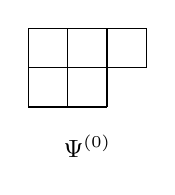
\begin{tikzpicture}
    \draw (0,0)--(1.5,0);
    \draw (0,-0.5)--(1.5,-0.5);
    \draw (0,-1)--(1,-1);
    \foreach \x in {0,0.5,1,1.5} 
    \draw (\x,0)--(\x,-0.5);
    \foreach \x in {0,0.5,1} 
    \draw (\x,-0.5)--(\x,-1);
    \draw (0.75,-1.5) node {\small $\Psi^{(0)}$};
  \end{tikzpicture}
  \quad
  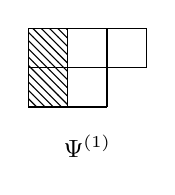
\begin{tikzpicture}
    \draw (0,0)--(1.5,0);
    \draw (0,-0.5)--(1.5,-0.5);
    \draw (0,-1)--(1,-1);
    \foreach \x in {0,0.5,1,1.5} 
    \draw (\x,0)--(\x,-0.5);
    \foreach \x in {0,0.5,1} 
    \draw (\x,-0.5)--(\x,-1);
    \draw[pattern=north west lines] (0,0) rectangle (0.5,-1);
    \draw (0.75,-1.5) node {\small $\Psi^{(1)}$};
  \end{tikzpicture}
  \quad
  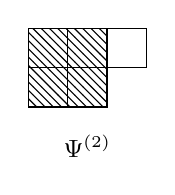
\begin{tikzpicture}
    \draw (0,0)--(1.5,0);
    \draw (0,-0.5)--(1.5,-0.5);
    \draw (0,-1)--(1,-1);
    \foreach \x in {0,0.5,1,1.5} 
    \draw (\x,0)--(\x,-0.5);
    \foreach \x in {0,0.5,1} 
    \draw (\x,-0.5)--(\x,-1);
    \draw[pattern=north west lines] (0,0) rectangle (1,-1);
    \draw (0.75,-1.5) node {\small $\Psi^{(2)}$};
  \end{tikzpicture}
  \caption{5=3+2}
  \label{fig:yangtu0}
\end{figure}
在图\ref{fig:yangtu0}中的第三个图$\Psi^{(2)}$,它表示在$\Psi^{(1)}$的基础上,再将$r_2$ 和$r_5$ 反对称化,所以$\Psi^{(2)}$ 也就是5个粒子按$3+2$ 分割时,所能达到的最大反对称程度.在以后的讨论中如果没有特殊声明,我们见到杨图\ref{fig:yangtu0}时应当按$\Psi^{(2)}$来理解,而不应当按变换中的状态$\Psi^{(0)},\Psi^{(1)}$理解,为了方便绘图,以后将不再绘出阴影.

下面按照$22=6+4+4+3+3+1+1$分割,我们来理解完整波函数区分成两部分乘积的时候,其构成对称和反对称的情形.

\begin{figure}[H]
  \centering
  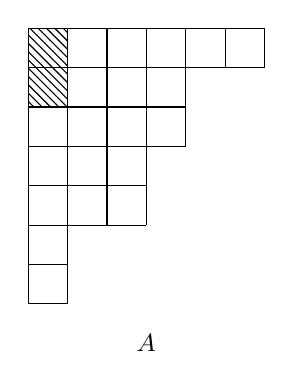
\begin{tikzpicture}
    \draw (0,0)--(3,0); 
    \draw (0,-0.5)--(3,-0.5); 
    \foreach \x in {0,0.5,1,1.5,2,2.5,3}
    \draw (\x,0)--(\x,-0.5);
    \foreach \x in {0,0.5,1,1.5,2}
    \draw (\x,-0.5)--(\x,-1.5);
    \draw (0,-1)--(2,-1);
    \draw (0,-1.5)--(2,-1.5);
    \foreach \x in {0,0.5,1,1.5}
    \draw (\x,-1.5)--(\x,-2.5);
    \draw (0,-2)--(1.5,-2);
    \draw (0,-2.5)--(1.5,-2.5);
    \foreach \x in {0,0.5}
    \draw (\x,-2.5)--(\x,-3.5);
    \draw (0,-3)--(0.5,-3);
    \draw (0,-3.5)--(0.5,-3.5);
    \draw (1.5,-4) node {\small $A$};
    \draw[pattern=north west lines] (0,0) rectangle (0.5,-1);
  \end{tikzpicture}
  \quad
  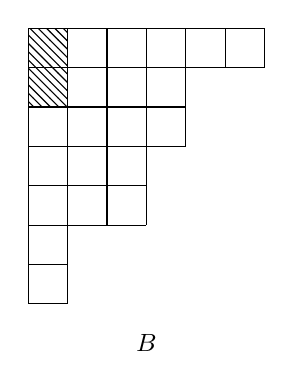
\begin{tikzpicture}
    \draw (0,0)--(3,0); 
    \draw (0,-0.5)--(3,-0.5); 
    \foreach \x in {0,0.5,1,1.5,2,2.5,3}
    \draw (\x,0)--(\x,-0.5);
    \foreach \x in {0,0.5,1,1.5,2}
    \draw (\x,-0.5)--(\x,-1.5);
    \draw (0,-1)--(2,-1);
    \draw (0,-1.5)--(2,-1.5);
    \foreach \x in {0,0.5,1,1.5}
    \draw (\x,-1.5)--(\x,-2.5);
    \draw (0,-2)--(1.5,-2);
    \draw (0,-2.5)--(1.5,-2.5);
    \foreach \x in {0,0.5}
    \draw (\x,-2.5)--(\x,-3.5);
    \draw (0,-3)--(0.5,-3);
    \draw (0,-3.5)--(0.5,-3.5);
    \draw (1.5,-4) node {\small $B$};
    \draw[pattern=north west lines] (0,0) rectangle (0.5,-1);
  \end{tikzpicture}
  \caption{整体对称波函数}
  \label{fig:yangtu1}
\end{figure}

在图\ref{fig:yangtu1}中,两部分波函数的杨图完全相同,在每一行中所填充相同的粒子的不同变量(比如坐标函数用A表示,自旋函数用B表示).记A和B的乘积AB,即
\begin{gather}
  \Psi^{(1)}=\Psi_A\cdot \Psi_B
\end{gather}
交换第一行第一列和第二行第一列的粒子时,$\Psi_A$ 和$\Psi_B$ 都改变一个负号,所以乘积AB将不变号.但是根据杨图的构成规则,A和B的行不具有交换对称性,所以如果交换同一行中的两个粒子,则乘积AB不具备交换对称性.然而粒子的每一种交换,相当于N个粒子在两张杨图中的同步分配,当我们考虑到所有置换后的乘积,然后再叠加起来,这个叠加之后的波函数包含了各种可能的交换,当交换两个同行的粒子时,相当于改变了一下两个乘积的顺序,由于加法的交换律它不影响波函数.所以这个所有分配方式的和构成整体的波函数,即
\begin{gather}
  \Psi=\sum_i\Psi^{(i)}
\end{gather}

\begin{figure}[H]
  \centering
  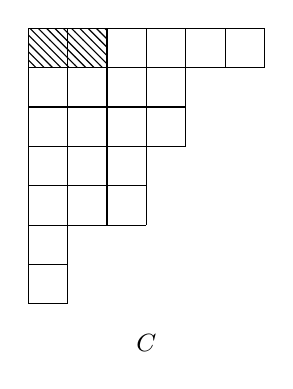
\begin{tikzpicture}
    \draw (0,0)--(3,0); 
    \draw (0,-0.5)--(3,-0.5); 
    \foreach \x in {0,0.5,1,1.5,2,2.5,3}
    \draw (\x,0)--(\x,-0.5);
    \foreach \x in {0,0.5,1,1.5,2}
    \draw (\x,-0.5)--(\x,-1.5);
    \draw (0,-1)--(2,-1);
    \draw (0,-1.5)--(2,-1.5);
    \foreach \x in {0,0.5,1,1.5}
    \draw (\x,-1.5)--(\x,-2.5);
    \draw (0,-2)--(1.5,-2);
    \draw (0,-2.5)--(1.5,-2.5);
    \foreach \x in {0,0.5}
    \draw (\x,-2.5)--(\x,-3.5);
    \draw (0,-3)--(0.5,-3);
    \draw (0,-3.5)--(0.5,-3.5);
    \draw (1.5,-4) node {\small $C$};
    \draw [pattern = north west lines](0,0) rectangle (1,-0.5);
  \end{tikzpicture}
  \quad
  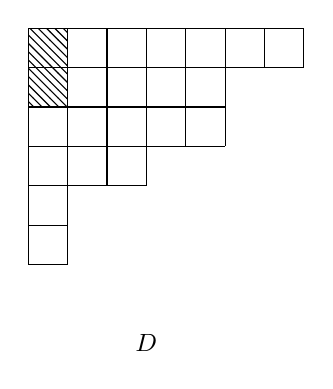
\begin{tikzpicture}
    \draw (0,0)--(3.5,0); 
    \draw (0,-0.5)--(3.5,-0.5); 
    \foreach \x in {0,0.5,1,1.5,2,2.5,3,3.5}
    \draw (\x,0)--(\x,-0.5);
    \foreach \x in {0,0.5,1,1.5,2,2.5}
    \draw (\x,-0.5)--(\x,-1.5);
    \draw (0,-1)--(2.5,-1);
    \draw (0,-1.5)--(2.5,-1.5);
    \foreach \x in {0,0.5,1,1.5}
    \draw (\x,-1.5)--(\x,-2);
    \draw (0,-2)--(1.5,-2);
    \foreach \x in {0,0.5}
    \draw (\x,-2)--(\x,-3);
    \draw (0,-2.5)--(0.5,-2.5);
    \draw (0,-3)--(0.5,-3);
    \draw (1.5,-4) node {\small $D$};
    \draw[pattern=north west lines] (0,0) rectangle (0.5,-1);
  \end{tikzpicture}
  \caption{整体反对称波函数}
  \label{fig:yangtu2}
\end{figure}

在图\ref{fig:yangtu2} 中,杨图C行所填充的粒子和杨图D列所填充的粒子是同一粒子的不同变量(比如C填充的是坐标变量,D填充的是自旋变量),当交换两个粒子时,比如交换C图中第一行第一列和第一行第二列坐标,则D图中的第一行第一列和第二行第一列也同时变换,如图中阴影所示.考虑C和D构成的乘积
\begin{equation}
  \Psi^{(j)}=\Psi_C\cdot\Psi_D
\end{equation}
当完成这样的交换后,乘积是变号的,但是行不具有对称性,如果像对称波函一样,我们求所有可能乘积的和,则这个和中包含了CD都是空白及如图阴影的形式,交换后每一个乘积改变一个负号,但是C行中的两个坐标由于是求和对称的,所以整体对称.当发生的交换是C中的两行,D中对应就是两列,整体和式对行变换对称,对列反对称,所以整体波函是反对称的.即
\begin{gather}
  \Psi=\sum_j\Psi^{(j)}
\end{gather}

综上所述我们可以得到,当一个整体波函的可以分为两部分时,将N个粒子分配到m个态中时,每一个杨图对应的物理情景是完全相同的(这是因为粒子的全同性造成的),而且即便是粒子在同一个杨图重新分配也不会造成什么不同,所以一个杨图对应一个能级.如果将两部分按AB组合再对各种分配求和,则整体波函将是对称的,用来描述玻色子;如果将两部分按CD组合(在朗道书中这种情况称为两个杨图具有{\bf 对偶关系}),再按各种分配求和,则整体波函将是反对称的,用来描述费米子.

下面考虑一个多电子系统,由于电子的自旋为$\frac{1}{2}$,所以它沿$z$ 的分量只能有$2s+1=2$个,因此描述电子自旋部分的杨图最多只能有两行,因为如果有三行,则反对称化列时,必然有一对相同,则造成波函为零.而对于行数,则由于是从对称出发的,所以对行数没有限制.而坐标波函数和自旋波函数构成整体波函数,电子是费米子,所以整体波函数由相互对偶的两个杨图确定,由于这个考虑,所以坐标波函只能是两列的杨图.引用朗道书中由四个电子构成的系统,其杨图为
\begin{figure}[H]
  \centering
  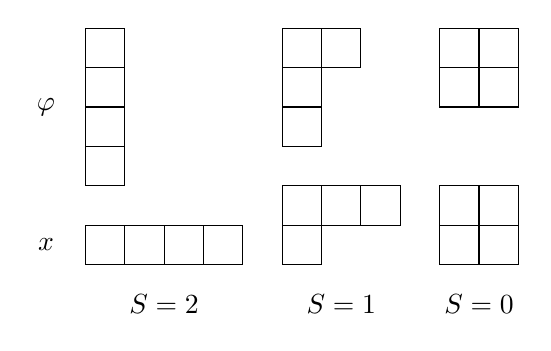
\begin{tikzpicture}
    \draw (-0.5,-1) node {$\varphi$};
    \draw (-0.5,-2.75) node {$x$};
    \draw (0,0) rectangle (0.5,-2); 
    \foreach \y in {-0.5,-1,-1.5}
    \draw (0,\y)--(0.5,\y);
    \draw (0,-2.5) rectangle (2,-3);
    \foreach \x in {0.5,1,1.5}
    \draw (\x,-2.5)--(\x,-3);
    \draw (2.5,0) rectangle (3,-1.5);
    \foreach \y in {-0.5,-1}
    \draw (2.5,\y)--(3,\y);
    \draw (3,0) rectangle (3.5,-0.5);
    \draw (2.5,-2) rectangle (4,-2.5);
    \foreach \x in {3,3.5}
    \draw (\x,-2)--(\x,-2.5);
    \draw (2.5,-2.5) rectangle (3,-3);
    \draw (4.5,0) rectangle (5.5,-1);
    \draw (5,0)--(5,-1);
    \draw (4.5,-0.5)--(5.5,-0.5);
    \draw (4.5,-2) rectangle (5.5,-3);
    \draw (5,-2)--(5,-3);
    \draw (4.5,-2.5)--(5.5,-2.5);
    \draw (1,-3.5) node {$S=2$};
    \draw (3.25,-3.5) node {$S=1$};
    \draw (5,-3.5) node {$S=0$};
  \end{tikzpicture}
  \caption{四个电子构成的杨图}
  \label{fig:4dianzi0}
\end{figure}

由图\ref{fig:4dianzi0}我们也可以明显的看出,一个杨图对应一个$S$值.如果考虑由自旋为$s$的全同粒子构成的系统,则也符合这个规则:一个杨图对就一个$S$值.粒子自旋为$s$值是,它的$z$轴分量有$2s+1$个,则杨图的行数不会超过$2s+1$.这里有一个特殊情况,如果粒子总数恰好为$2s+1$的整数倍,即$N(2s+1)$个,则杨图中有一个是每列是$2s+1$格,每行$N$格的矩形图,这图的总角动量$S$ 显然为0.同时考虑到两个角动量的合成,一个粒子角动量为$s_1$,另一个为$s_2$,则合成时的总角动量可能为:$s_1-s_2$, $s_1-s_2+1$ ,$\cdots$,$s_1+s_2$.所以只有当两个角动量值相同时,总角动量值才有可能为零,即$s_1=s_2$,时,最低总角动量值$s_1-s_2=0$.

两个多粒子系统,如果它们的总自旋为零,则表明两个系统的自旋值是相同.反应到杨图中就是两个杨图构成{\bf 互补杨图}.这里的互补,我们应当这样理解:一个杨图可以按行由多到少按左对齐排列,也可以按行由少到多右对齐排列,它们只是有一个排列形式上的不同,不会影响到对称性,所以是等价的.一个粒子系统的杨图按行由多到少左对齐排列,另一个粒子系统的杨图按行由少到多,右对齐排列,则两个杨图可以构成一个矩形.例如当$s=1$时,两个系统A和B,A由7个粒子构成,B由5个粒子构成,则考虑整体AB有12个粒子.符合粒子数是$2s+1$的倍数的关系,即
\begin{gather}
  \frac{12}{2\times 1+1}=4
\end{gather}
所以整体这个大系统$S$为零的时候构成一个$3\times4$ 的矩形杨图.如图\ref{fig:hubuyangtu}中所示,7个由实线表示的格为系统A,5个由虚线表示的格为系统B,则它们构成互补杨图,不难验证两种情况下的自旋相等关系.

\begin{figure}[H]
  \centering
  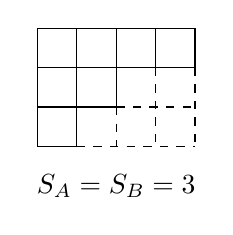
\begin{tikzpicture}
    \draw (0,0) rectangle (2,-0.5);
    \foreach \x in {0.5,1,1.5}
    \draw (\x,0)--(\x,-0.5);
    \draw (0,-0.5) rectangle (1,-1);
    \draw (0.5,-0.5)--(0.5,-1); 
    \draw (0,-1) rectangle (0.5,-1.5);
    \draw[dashed] (1,-1)--(2,-1);
    \draw[dashed] (0.5,-1.5)--(2,-1.5);
    \draw[dashed] (1,-1)--(1,-1.5);
    \draw[dashed] (1.5,-0.5)--(1.5,-1.5);
    \draw[dashed] (2,-0.5)--(2,-1.5);
    \draw (1,-2) node {$S_A=S_B=3$};
  \end{tikzpicture}
  \quad
  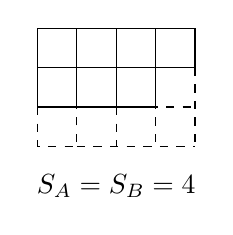
\begin{tikzpicture}
    \draw (0,0) rectangle (2,-0.5);
    \foreach \x in {0.5,1,1.5}
    \draw (\x,0)--(\x,-0.5);
    \draw (0,-0.5) rectangle (1.5,-1);
    \draw (0.5,-0.5)--(0.5,-1); 
    \draw (1,-0.5)--(1,-1); 
    \draw[dashed] (0,-1) rectangle (0.5,-1.5);
    \draw[dashed] (1,-1)--(2,-1);
    \draw[dashed] (0.5,-1.5)--(2,-1.5);
    \draw[dashed] (1,-1)--(1,-1.5);
    \draw[dashed] (1.5,-0.5)--(1.5,-1.5);
    \draw[dashed] (2,-0.5)--(2,-1.5);
    \draw (1,-2) node {$S_A=S_B=4$};
  \end{tikzpicture}
  \caption{互补杨图}
  \label{fig:hubuyangtu}
\end{figure}

下面讨论两个重要的问题.其一,自旋变量组成的杨图与自旋一般而言不是一一对应的.下面以课后题第2题来说明之.

2.系统由自旋为1的粒子组成,求种对称类型的自旋函数所具有的总自旋值$S$,设系统的粒子数为$2,3,4$.

{\bf 解:} 对双粒子系统,这个对应关系由下列事实所确立:粒子对换后,自旋波函数就乘以$(-)^{2s-S}$.对于$s=1$的粒子,由此得
\begin{figure}[H]
  \centering
  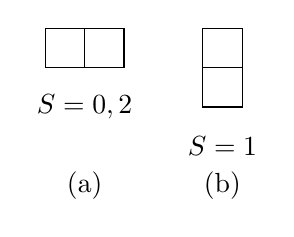
\begin{tikzpicture}
    \foreach \x in {0,0.5}
    \draw (\x,0)++(0.5,-0.5) rectangle (\x,0);
    \draw (0.5,-1) node {$S=0 , 2$};
    \draw (0.5,-2) node {(a)};
    \foreach \y in {0,-0.5}
    \draw (2,\y)++(0.5,-0.5) rectangle (2,\y);
    \draw (2.25,-1.5) node {$S=1$};
    \draw (2.25,-2) node {(b)};
  \end{tikzpicture}
  \caption{2个自旋为1的粒子}
  \label{fig:twobose}
\end{figure}
对于图\ref{fig:twobose}我们可以做如下理解:由两个粒子构成的杨图只能有这两个形式.按角动量合成规则,两个自旋为1的粒子合成,其总自旋可能值为0,1,2 .(a)波函数满足对称性,所以它只能对应$S=0$ 或者$S=2$.这里需要做出解释,为什么会有这个结果?由于自旋为1,所以杨图不会超过$2s+1=3$ 行,而这三行分别对应三个不同的$z$分量 $1$,$0$,$-1$.而这两个格只占一行,所以它可以是这三行中的任何一行,所以它所对应的$z$轴分量可以是$1+1=2$,$0+0=0$,$-1-1=-2$.总自旋为$0,1,2$ 的情况都可能出现$S_z=0$,总自旋为$2$的情况才可能有$S_z=2$,而交换对称性限定了只能$S$为偶数,所以只能是$S=0,2$.(b)满足反对称性,所以只能对应$S=1$. 这里也需要解释一下,此杨图可以对应的是三个不同$z$分量的前两行,也可心介后两行,这两种情况分别给出$S_z=1$ 和$S_z=-1$,而可以给出$S_z=\pm 1$ 的总自旋值只能是$S=1,2$,而反对称性限定了$S=1$.

对于三个粒子的情况,我们可以在2个粒子的基础上再添加一个格,具体过程参见朗道书222页,这里主要的目的是讨论结果,结果为

\begin{figure}[H]
  \centering
  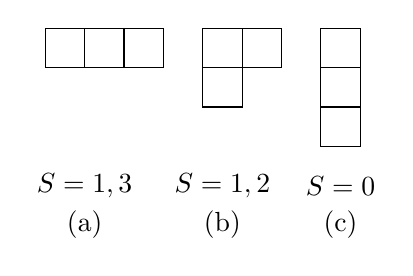
\begin{tikzpicture}
    \foreach \x in {0,0.5,1}
    \draw (\x,0)++(0.5,-0.5) rectangle (\x,0);
    \draw (0.5,-2) node {$S=1 , 3$};
    \draw (0.5,-2.5) node {(a)};
    \foreach \y in {0,-0.5}
    \draw (2,\y)++(0.5,-0.5) rectangle (2,\y);
    \draw (2.5,0)++(0.5,-0.5) rectangle (2.5,0);
    \draw (2.25,-2) node {$S=1 ,2$};
    \draw (2.25,-2.5) node {(b)};
    \foreach \y in {0,-0.5,-1}
    \draw (3.5,\y)++(0.5,-0.5) rectangle (3.5,\y);
    \draw (3.75,-2) node {$S=0$};
    \draw (3.75,-2.5) node {(c)};
  \end{tikzpicture}
  \caption{3个自旋为1的粒子}
  \label{fig:threebose}
\end{figure}

图\ref{fig:threebose} 中(a)占据一行,所以它可是占据$s_z=1,0,-1$ 的任何一行,因此总的自旋的$z$分量可能是$S_z=0,\pm 3$ ,这样的$z$分量可以由$S=0,1,2,3$产生,但是注意,这个杨图是由两个粒子的杨图\ref{fig:twobose}中的(a)演变来的,而那时的$S=0,2$,按角动量的合成,只能产生$S=1,3$ 的情况,因此图\ref{fig:threebose} 中的(a)所示的只能是$S=1,3$.还需要注意,双粒子系统,粒子交换后符号变化$(-)^{2s-S}$,但是对于三个及以上的粒子没有这个要求,所以这里的$S=1,3$ 是允许的.图\ref{fig:threebose}中(b)占据两行,可以是上两行也可以是下两行,所以它对应的总自旋$z$分量可以是$S_z=2,\pm 1$ ,产生这个分量的总自旋可以是 $S=1,2,3$,然而这个\ref{fig:threebose}中(b)也可以来源于图\ref{fig:twobose}中的(b),由角动量的合成规则,这个总自旋只能是$0,1,2$,图\ref{fig:threebose}中(b)必须同时满足这两个情况,因此其$S$值应当是按这两种情况得到的,重合的$S$值,所以其只能是$S=1,2$.图\ref{fig:threebose}中(c)只是从图\ref{fig:twobose}中(b)演变而来,其对应于$S=0,1,2$而已经判断出来\ref{fig:threebose}中(b)表示的是$S=1,2$,因此(c)必然对应$S=0$.

对于4个粒子的情况,我们可以按朗道书中的方法继续做出来,但是在这里不再继续引用.而讨论杨图所代表的$S$值时,可以按朗道书中的方法,也可以按照此处我的讨论方式.这里明确一点的是:一个杨图必定对应一个确定的$S_z$值,这个$S_z$值可以由大于等于它的不同的$S$值产生,所以一般而言,杨图与$S$值不是一一对应的.

下面再来讨论第二个问题:一个系统由自旋为$s$的粒子构成,当粒子总数为$2s+1$的整数倍时,即$N(2s+1)$个粒子,其所有的杨图中那个$(2s+1)\times N$的矩形杨图对应的总角动量为$0$.\footnote{这个问题于2019年7月14日思考一天,终于想通,记于此处.}

总自旋可以表为升降算符的形式,这个在$S_z$表像中求$\hat{S}^2$的本征值的做法一致.即
\begin{gather}
  \hat{S}^2=S_-S_++S_z^2+\hbar S_z
\end{gather}
对于这个矩形杨图显然理解为$S_z$表像中的情况,而算出$S_z=0$.同时升降算子会导致$m$值发生增减,但是每一个粒子它包含了所有$s_z$值,当$S_\pm=\sum s_\pm$作用到它上时,必然会在作用的分量上替换为其相差1的一个态,由于占据了所有的态,所以必然导致出现两个相同的态在同一列上.则

\begin{gather}
  \left<S_-S_+\right>=0
\end{gather}
于是可以判断
\begin{gather}
  \left<\hat{S}^2\right>=0
  \intertext{即}
  S(S+1)=0
\end{gather}
所以可以判断这个杨图对应的总自旋是唯一的,即$S=0$.

这个问题,也可以这样理解.杨图并没有指明表像.但是这指明了一个实际存在的状态,一个物理量的量子平均值与表像无关.这个 $(2s+1)\times N$ 的杨图,在 $S_z$  表像中理解,则显然有$S_z=0$ ,则$\left < S_z^2 \right >=0 $,同理,这个杨图也可以认为是在$S_x$表像中理解,则显然也对就$\left<S_x^2 \right>=0$,同理理解为在$S_y$表像中可得$\left<S_y^2\right>=0$,于是可以得到
$  S(S+1)=\left<S_x^2\right>+\left<S_y^2\right>+\left<S_z^2\right>=0$,
于是同样得出结论:此矩形杨图对应总自旋为0.\footnote{此处的理解是在2019年7月15日打这篇稿子时临时想到的.}

由$N(2s+1)$个自旋为$s$构成的矩形杨图对应的总自旋为0,我们可以推断出一个重要结论:自旋为$\frac{1}{2}$的粒子所构成的杨图与总自旋也一一对应.原因在于,自旋为$\frac{1}{2}$粒子所构成的杨图不会超过两行.同时一个单行的杨图必然对应一个确定的角动量,比如5个自旋为$\frac{1}{2}$的粒子构成的系统,其中排成一行的杨图如图\ref{fig:0.5fermi}所示.
\begin{figure}[H]
  \centering
  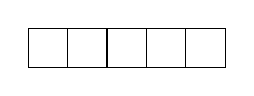
\begin{tikzpicture}
    \foreach \x in {0,0.5,1,1.5,2}
    \draw (\x,0)++(0.5,-0.5) rectangle (\x,0);
  \end{tikzpicture}
  \caption{单行1/2自旋粒子构成的系统}
  \label{fig:0.5fermi}
\end{figure}
显然此杨图所对应的总自旋$z$分量为$\frac{5}{2}$,而最大的角动量也就是$S=\frac{5}{2}$,所以此杨图对应的也只能是最大的角动量,即自旋$\frac{1}{2}$粒子构成单行杨图对应它些粒子所能构成的最大角动量,它是唯一的.

当然这5个粒子,还有其它的杨图,如图\ref{fig:0.5fermi0}所示
\begin{figure}[H]
  \centering
  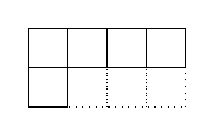
\begin{tikzpicture}
    \foreach \x in {0,0.5,1,1.5}
    \draw (\x,0)++(0.5,-0.5) rectangle (\x,0);
    \draw (0,-0.5) rectangle (0.5,-1);
    \foreach \x in {0.5,1,1.5}
    \draw [dotted] (\x,-0.5)++(0.5,-0.5) rectangle (\x,-0.5);
  \end{tikzpicture}
  \caption{两行1/2自旋粒子构成的系统}
  \label{fig:0.5fermi0}
\end{figure}
不难判断出来,互补杨图是一个单行的3格杨图,而这个单行3格杨图按前述规则,它对就一个$S'=\frac{3}{2}$的系统,而$N(2s+1)$个自旋为$s$的粒子构成的矩形杨图对应总自旋为0,按角动量的合成规则,只有两个角动量值相等的时候才会合成出总自旋为0的情况,于是互补杨图具有相同的$S$值,所以此处的5个自旋为$\frac{1}{2}$粒子所组成的系统其总自旋为$S=\frac{3}{2}$.按照这个规则一直继续下去,每一个二行杨图的互补杨图都是一个单行杨图,所以可得出结论:对于$\frac{1}{2}$粒子构成的系统,每一个杨图与总自旋是一一对应的.但是自旋不为$\frac{1}{2}$的粒子所构成的系统情况不一定成立.

\section{二次量子化---玻色统计}

设$\hat{f}^{(1)}_a$ 是粒子a的某个物理量算符,它只作用在$\xi_a$的函数上.我们可以计算出$\hat{f}^{(1)}_a$的矩阵得
\begin{gather}
  \hat{f}^{(1)}_a \psi_{p_k}(\xi_a)=\sum_l \psi_{p_l}(\xi_a)f_{lk} 
  \label{eq:twoliangzihua0}
  \intertext{上式中矩阵$f_{lk}$中省去了符号$a$,由于此矩阵与计算用的坐标无关,所以可以略去下标.即}
  f_{lk}=\int \psi_{p_l}^*(\xi) \hat{f}^{(1)}\psi_{p_k}(\xi) \mathrm{d}\xi
\end{gather}
由式\eqref{eq:twoliangzihua0}可得,当$\hat{f}^{(1)}_a$ 作用在波函$\psi_{p_k}$上时,右式可以认为是用各本征波函数展开.同时,也可以视为将波函数$\psi_{p_k}$分别取代为$\psi_{p_l}f_{lk}$,这在占有数表像中十分重要.对于由$N$个Bose 子构成的系统,波函可以写为
\begin{gather}
\left| N_1N_2\cdots \right>  
=\sqrt{\frac{N_1!N_2!\cdots}{N!}}
\sum \psi_{p_1}(\xi_1)\psi_{p_2}(\xi_2)\cdots
\end{gather}
记$\hat{F}^{(1)}$为
\begin{equation}
  \hat{F}^{(1)}=\sum_a \hat{f}^{(1)}_a
\end{equation}
将$\hat{F}^{(1)}$作用于占有数表像得
\begin{align}
  \sum_a \hat{f}^{(1)}_a \left|N_1N_2\cdots\right>&=
  \sqrt{\frac{N_1!N_2!\cdots}{N!}}
  \left\{ f_{1k}\sum \psi_{p_k}(\xi_1)\psi_{p_2}(\xi_2)\cdots\notag\right.\\
    &+f_{2k}\sum \psi_{p_1}(\xi_1)\psi_{p_k}(\xi_2)\cdots\notag\\
    &\cdots\cdots \notag\\
    &\left.+f_{Nk}\sum \psi_{p_1}(\xi_1)\psi_{p_k}(\xi_2)\cdots\psi_{p_k}(\xi_N)\right\}
\end{align}
我们考虑非零矩阵元,显然对角元不为零.下面计算之,由于在$\hat{F}^{(1)}$中对所有的坐标变量求和,则从$\psi_{p_i}$到$\psi_{p_i}$的变换一共有$N_i$项,原因在于有$N_i$个态是相同的.所以对角元为
\begin{gather}
  \left< N_i\left|\sum_a \hat{f}^{(1)}_a \right|N_i\right>=f_{ii}N_i
\end{gather}
当$\hat{F}^{(1)}$作用于某个量子态上时,相当于将此量子态消灭而重新取代了不同的态,以相同态取代的情况,上面已经求出来了.下面求出取代为不同的态的矩阵元,显然只有下列矩阵元不为零
\begin{gather}
  \left< N_i,N_k-1\left|\sum_a \hat{f}^{(1)}_a \right|N_i-1,N_k\right>=
  f_{ik} \sqrt{\frac{N_i!(N_k-1)!\cdots}{N!}}\sqrt{\frac{(N_i-1)!N_k!\cdots}{N!}}
  N_k \frac{N!}{(N_i-1)!N_k!\cdots}\notag
  \intertext{经过简单计算可得}
  \left< N_i,N_k-1\left|\sum_a \hat{f}^{(1)}_a \right|N_i-1,N_k\right>=
  f_{ik}^{(1)}\sqrt{N_iN_k}
\end{gather}

在线性谐振子中,我们遇到了升算符$\hat{a}^+$和降算符$\hat{a}$,同时有
\begin{gather}
  \left\{
    \begin{gathered}
      \hat{a}\left|n+1\right>=\sqrt{n}\left|n\right>\\
      \hat{a}^+\left|n\right>=\sqrt{n}\left|n+1\right>
    \end{gathered}
  \right.
\end{gather}
类比线性谐振子的情况,这里可以对每一个变量引入对应的升降算符
\begin{gather}
 \left\{
   \begin{gathered}
     \hat{a}_i\left|N_1,N_2,\cdots,N_i,\cdots\right>=\sqrt{N_i}\left|N_1,N_2,\cdots,N_i-1,\cdots\right>\\
     \hat{a}_i^+\left|N_1,N_2,\cdots,N_i,\cdots\right>=\sqrt{N_i+1}\left|N_1,N_2,\cdots,N_i+1,\cdots\right>
   \end{gathered}
   \right.
\end{gather}
则显然可以将$\hat{F}$表达为
\begin{equation}
  \hat{F}^{(1)}=\sum_{ik} f^{(1)}_{ik}\hat{a}_i^+\hat{a}_k
\end{equation}
这个式子之所以完全等价,原因在于据其所计算的矩阵元和直接计算的结果完全相同,但是相比直接计算,用此升降算符计算更加方便.上述结果可以方便的推广到多粒子的情况,并且计算起来可以比直接计算方便的多.比如如下替换
\begin{gather}
     \hat{F}^{(2)}=\sum_{a>b}\hat{f}^{(2)}_{ab}\notag\\
     \hat{F}^{(2)}=\frac{1}{2}\sum_{i,k,l,m}\left<ik\right|\hat{f}^{(2)}\left |lm\right>
     \hat{a}_i^+\hat{a}_k^+\hat{a}_l\hat{a}_m
\end{gather}

下面讨论整体的降算符和升算符.一个$N-1$的占有数表像可以用$N$个占有数表像,每个量子态依次减少1所形成的$N-1$个占有数的表像的线性叠加.记$N-1=N_1'+N_2'+\cdots +N_m'$,即
\begin{equation}
  \left|N_1'N_2'\cdots N_m'\right>
  =C_1\left|N_1-1,N_2,\cdots,N_m\right>
  +C_2\left|N_1,N_2-1,\cdots,N_m\right>
  +\cdots
  +C_m\left|N_1,N_2,\cdots,N_m-1\right>
  \notag
\end{equation}
在上式中各个展开系数尚未确定,这里考虑的依据是都是占有数表像,没有哪一个量子态是特殊的,所以按等概率可以考虑到每一个占有数表像出现的概率与本占有数表像的粒子数成正比.于是可得
\begin{align}
  \sqrt{N}\left|N_1'N_2'\cdots N_m'\right>
  &=\psi_1(\xi)\sqrt{N_1}\left|N_1-1,N_2,\cdots,N_m\right>\notag\\
  &+\psi_2(\xi)\sqrt{N_2}\left|N_1,N_2-1,\cdots,N_m\right>
  +\cdots
  +\psi_m(\xi)\sqrt{N_m}\left|N_1,N_2,\cdots,N_m-1\right>
  \notag
\end{align}
上式中$\psi_i(\xi)$为比例系数.于是可以引入整体降算符$\hat{\Psi}$,则
\begin{equation}
  \hat{\Psi}=\sum_{i=1}^m \psi_i(\xi)\hat{a}_i
  \label{eq:totaljiangfu}
\end{equation}
于是得
\begin{equation}
  \hat{\Psi}\left|N\right>=\sqrt{N}\left|N-1\right>
  \label{eq:totaljiangfu0}
\end{equation}
对于$\hat{\Psi}$取共轭可得$\hat{\Psi}^+=\sum_{i=1}^m \psi_i^*\hat{a}_i^+$,作用于波函数得
\begin{equation}
  \hat{\Psi}^+\left|N-1\right>=\sqrt{N}\left|N\right>
  \label{eq:totaljiangfu1}
\end{equation}
在$\hat{\Psi}$中,各$\psi_i(\xi)$为相互正交的波函数,则$\hat{F}^{(1)}$可以表达为
\begin{equation}
  \hat{F}^{(1)}=\int \hat{\Psi}^+(\xi) \hat{f}^{(1)}\hat{\Psi}(\xi)\mathrm{d}\xi
  \label{eq:totaljiangfu2}
\end{equation}

根据所引入的$\hat{\Psi}$可以得出粒子密度算符$\hat{\Psi}^+(\xi)\hat{\Psi}(\xi)$,则考虑积分
\begin{equation}
  \hat{N}=\int \hat{\Psi}^+(\xi)\hat{\Psi}(\xi)\mathrm{d}\xi=\sum_i \hat{a}^+_i\hat{a}_i
  \label{eq:totaljiangfu3}
\end{equation}
上式中$\hat{N}$即是粒子数算符.

\section{二次量子化---费米统计情形}

当有$N$个费米子时,各粒子的坐标分别以$\xi_i$来表示,其满足反对称性波函数为
\begin{equation}
  \Psi (n_1,n_2,\cdots,n_N)=\frac{1}{\sqrt{N!}}
  \begin{vmatrix}
    \Psi_{p_1}(\xi_1)&\Psi_{p_1}(\xi_2)&\cdots&\Psi_{p_1}(\xi_N)\\
    \Psi_{p_2}(\xi_1)&\Psi_{p_2}(\xi_2)&\cdots&\Psi_{p_2}(\xi_N)\\
    &&\vdots &\\
    \Psi_{p_N}(\xi_1)&\Psi_{p_N}(\xi_2)&\cdots&\Psi_{p_N}(\xi_N)
  \end{vmatrix}
\end{equation}
由于同行时行列式为零,所以不可能同一时刻有两个以上粒子处于相同的态.所以粒子的占有数要么为1要么为0,则如果超过了N个粒子,则其余的粒子占有数为0,如下表示
\footnote{此处参考了《高等量子力学》 杨泽森 著,北京大学出版社,第三版.}
\begin{equation}
  \left|N_1,N_2,\cdots\right>=\Psi(n_1,n_2)
  \qquad
  N_1=N_2=1,N_3=N_4=\cdots =0
  \label{eq:twoliangzifermi}
\end{equation}
下面直接计算$\hat{F}^{(1)}=\sum_a \hat{f}_a^{(1)}$的非零矩阵元.其中对角元显然是非零的,即
\begin{equation}
  \left<1_i\right|\hat{F}^{(1)}\left|1_i\right>=f_{ii}
  \label{eq:ercifermi0}
\end{equation}
显然上式对于$0_i$的对角元为零,所以可以写为与玻色子相同的形式为
\begin{equation}
  \left<N_i\right|\hat{F}^{(1)}\left|N_i\right>=f_{ii}N_i
  \label{eq:ercifermi1}
\end{equation}
同时,使一个占有数($N_i$)减少一个(从1变到零)另一个占有数($N_i$)增加一(从零变到1)的那些跃迁矩阵元才不等于零.当$i<k$时,显然
可得$\hat{F}^{(1)}\left|0_i,1_k\right>$ 考虑到将$\phi_{p_k}(\xi_k)$转换到$\phi_{p_i}$态组成新的行列式,然后变换行使$\phi_{p_i}$达到正常的位置(即下标按从小到大排列),这中间需要交换的行数就等于从$i+1$到$k-1$中的不为零的行数,这些不为零的行数上占有数为$1$,所以将$i+1$到$k-1$之间的所有占有数求和,则为零的那些占有数不起作用,只有占有数为$1$的那些态起作用.同时,由于一个量子态上最多有一个量子态,则不会像玻色子那样有根号项.出现的因素只能是符号项和$\hat{f}^{(1}$的矩阵元.从$i+1$ 到$k-1$ 内占有数之和记为$\sum (i+1,k-1)$,显然可得非对角非零矩阵元为
  \begin{equation}
    \left<1_i,0_k\right|\hat{F}^{(1)}\left|0_i,1_k\right>=f^{(1)}_{ik}(-)^{\sum (i+1,k-1)}
    \label{eq:ercifermi2}
  \end{equation}

  为了把算符$\hat{F}^{(1)}$也表达为类似升降算符的形式,则定义两个算符为
  \begin{equation}
    \left<0_i\right|\hat{a}_i \left|1_i\right>=\left<1_i\right|\hat{a}^+_i\left|0_i\right>=(-)^{\sum (1,i-1)}
    \label{eq:ercifermi3}
  \end{equation}
  所以两个矩阵相乘,当$i<k$时可得
  \begin{align}
    \left<1_i,0_k\right|\hat{a}_i^+\hat{a}_k\left|0_i,1_k\right>&=\left<1_i,0_k\right|\hat{a}_i^+\left|0_i,0_k\right>\left<0_i,0_k\right|\hat{a}_k\left|0_i,1_k\right>\notag\\
    &=(-)^{\sum (1,i-1)}(-)^{\sum (1,i-1)+\sum (i+1,k-1)}\notag
    \intertext{也即}
    \left<1_i,0_k\right|\hat{a}_i^+\hat{a}_k\left|0_i,1_k\right>&=(-)^{\sum (i+1,k-1)}
    \label{eq:ercifermi4}
  \end{align}
  按照$\hat{a}$在此处的定义可得
  \begin{equation}
    \hat{a}_i^+\hat{a}_i=N_i
    \label{eq:ercifermi5}
  \end{equation}
  同理交换$i,k$可得
  \begin{equation}
    \left<1_i,0_k\right|\hat{a}_k\hat{a}_i^+\left|0_i,1_k\right>=-(-)^{\sum (i+1,k-1)}
    \label{eq:ercifermi6}
  \end{equation}
  由式\eqref{eq:ercifermi6}和式\eqref{eq:ercifermi4}相加可得
  \begin{equation}
    \hat{a}_i^+\hat{a}_k+\hat{a}_k\hat{a}_i^+=0 ,\qquad i\neq k
    \label{eq:ercifermi7}
  \end{equation}
  同时可以求得
  \begin{equation}
    \hat{a}_i\hat{a}_i^+=1-N_i
    \label{eq:ercifermi8}
  \end{equation}
  同\eqref{eq:ercifermi1}对比可得
  \begin{equation}
    \hat{a}_i\hat{a}_i^++\hat{a}_i^+\hat{a}_i=1
    \label{eq:ercifermi9}
  \end{equation}
  综合式\eqref{eq:ercifermi9}和式\eqref{eq:ercifermi7}可得
  \begin{equation}
    \hat{a}_i^+\hat{a}_k+\hat{a}_k\hat{a}_i^+=\delta_{ik}
    \label{eq:ercifermi10}
  \end{equation}


\chapter{狭义相对论}
%2019年 07月 24日 星期三 13:58:34 CST 
近几天研究狭义相对论,我的原始教材是郭硕鸿先生的《电动力学》(第二版),同时在学习过程中又参考过一些其它的教材.学习完成后总感觉理解的不是很到位,或者这也和工作繁忙没有时间集中时间研究有一定关系,但是我自己认为这个关系不大.在理论物理的学习过程中遇到了很多困难,经过努力逐步攻克了这些困难.最终我选择了朗道十卷作为我的主攻教材,这套书给了我很多逻辑清析,认识深刻的知识,对于相对论而言,朗道的论述是十分独到的.在此,我根据自己的学习理解,作了这一章的学习笔记.

\section{相互作用的传播速度}

\subsection{参考系}

描述自然界中所发生的现象需要有一个作为参考的物体,这个物体叫做\CJKunderwave{参考系}.在各种各样的参考系中有一个特殊的参考系,在此参考系中一个不受外力作用的物体将做匀速直线运动,这个参考系叫做\CJKunderwave{惯性参考系}.

\subsection{相对性原理}

\CJKunderwave{实验表明}所有的自然定律在所有惯性系中都是相同的.即表示自然定律的方程对于一个惯性系到另一个惯性系的时间与坐标的变换来说表达形式上是相同的.这个规律也是显然的,自然规律不应当与选择的参考系有关,唯一不同的可能是数值,但是函数关系应当是相同的.

\subsection{最大传播速度}

自然界中存在相互作用的两个物体,实验表明当其中一个物体发生任何变动时,仅仅只在某段时间以后才能被相互作用的另一个物体感知.我们以两个物体的距离除以从一个物体发生变动与另一个物体感知所用时间,得到相互作用的传播速度.当它们可以有多种方式相互作用时(比如同时有万有引力和电磁相互作用力),不同的作用有不同的传播速度.在某一参考系中我们可以找到一个最大的传播速度.当转换到另一个惯性系中时,这些传播速度会发生变化.但是我们不知道它是变大还是变小.假设两个惯性系A和B,在A中的最大传播速度为$v_{Amax}$,在B中的最大传播速度为$v_{Bmax}$,假设由A变换到B时,这个最大的传播速度变大了,则有$v_{Bmax}>v_{Amax}$,但是按照相对性原理从B变换到A时最大传播速度也应当变大了,所以得出$v_{Amax}>v_{Bmax}$显然二种情况是矛盾的,然而相对性原理是正确的,所以就得到在不同的惯性参考系中最大的传播速度必然相同.即$v_{Amax}=v_{Bmax}$,我们记此最大传播速度为$c$,则在所有的惯性系中它都是不变的.

从一个粒子向另一个粒子传播的相互作用往往又叫做``信号'',所以相互作用的传播速度又称为\CJKunderwave{信号速度}.这个最大的信号速度$c$就是光束,真空中的数值为
\begin{equation}
  c=2.998\times 10^8 m/s
  \label{eq:signalmax}
\end{equation}

\section{间隔}

在相对论中描述一个现象,我们需要指明它发生的地点和时间,这称为一个事件.即事件用一个四维坐标$(t,x,y,x)$来描述.在这个描述事件的四维空间中,一个事件对应到一组坐标,这组坐标称为四维空间中的一个点,因此我们可以说事件可以用点来表示,这个点叫做\CJKunderwave{世界点}.在假想的四维空间中,一个粒子对应若干个世界点,比如一个静止的粒子,在三维空间中它没有动,但是在四维空间中,它的时间坐标是一直增加的,由这些世界点连起来构成一条``曲线'',叫做\CJKunderwave{世界线}.一个做匀速直线运动的粒子,它各个坐标的比值都相同,所以可以说它的世界线是一条直线.一个做曲线运动的粒子,它的四维描述也是一系列的世界点,但是由于是曲线运动,则各坐标的比值不会是相同的,所以它的世界线也是曲线.

我们来研究光速在不同参考系中的测量.选定一个参考系$O$,在其中测量光速,事件1为光在此位置$(t_1,x_1,y_1,z_1)$发出,事件2为光在$(t_2,x_2,y_x,z_2)$接收.于是
\begin{equation}
c^2(t_2-t_1)^2-)(x_2-x_1)^2-(y_2-y_1)^2-(z_2-z_1)^2=0
  \label{eq:Olight0}
\end{equation}
选定第二个参考系$O'$,事件1为光在此位置$(t'_1,x'_1,y'_1,z'_1)$发出,事件2为光在$(t'_2,x'_2,y'_x,z'_2)$接收.于是
\begin{equation}
c^2(t'_2-t'_1)^2-)(x'_2-x'_1)^2-(y'_2-y'_1)^2-(z'_2-z'_1)^2=0
  \label{eq:Olight1}
\end{equation}
如果事件1和事件2不是以光速相联系,则上式必然就不等于零.同时由于光速是最大的信号速度,所以以上二式都应当大于等于零.记
\begin{equation}
  s_{12}=\sqrt{c^2(t_2-t_1)^2-(x_2-x_1)^2-(y_2-y_1)^2-(z_2-z_1)^2}
  \label{eq:jiange0}
\end{equation}
则$s_{12}$称为两个事件的间隔,显然有$s_{12}\geqslant 0$.为了讨论方便,我们取事件为在原点上,则间隔可以表达为
\begin{equation}
  s=\sqrt{c^2t^2-x^2-y^2-z^2}
  \label{eq:jiange}
\end{equation}

\subsection{朗道关于间隔不变性的论述}

下面讨论当坐标系变换后,间隔的变换规则.由于我们不知道$s^2$和$s'^2$的关系,所以我们可以假设其存在未知的函数关系,当$s^2$取微小变量$ds^2$时,则可以按$ds'^2$ Taylor展开.由于在测量光速中,当$s'^2=0$时$s^2=0$,所以展开的首项为0.则有下式成立
\begin{equation}
  ds^2=ads'^2
  \label{eq:jiange1}
\end{equation}
系数$a$ 只能与$O$和$O'$之间的相对运动的速度的大小有关.因为从$O$中的任何的一个世界点都可以做为起点,任何一个世界点都可以做为终点,只要二个世界点间的间隔相同,则在$O'$中也应当有相同的变换,这构成了惯性系的均匀性.如果$a$与速度的方向有关,则就与这里所述的惯性空间的均匀性相矛盾了.于是对于$O$和$O'$惯性系有
\begin{equation}
  ds^2=a(v_{1})ds'^2
  \label{eq:jiange2}
\end{equation}
同理对于$O$和$O''$惯性系有
\begin{equation}
  ds^2=a(v_{2})ds''^2
  \label{eq:jiange3}
\end{equation}
而对于$O'$和$O''$惯性系有
\begin{equation}
  ds'^2=a(v_{12})ds''^2
  \label{eq:jiange4}
\end{equation}
由式\eqref{eq:jiange2}和\eqref{eq:jiange3}联立可得
\begin{equation}
  ds'^2=\frac{a(v_{1})}{a(v_{2})}ds''^2
  \label{eq:jiange5}
\end{equation}
对比式\eqref{eq:jiange4}和式\eqref{eq:jiange5}可得
\begin{equation}
  a(v_{12})=\frac{a(v_{1})}{a(v_{2})}
  \label{eq:jiange6}
\end{equation}
在式\eqref{eq:jiange6}中左中含有$\vec{v}_1$和$\vec{v}_2$的夹角,但是在右式中不含有角度的信息,所以可以得到$a$只能是一个常数,所以由式\eqref{eq:jiange6}可得$a=1$.所以对于微小间隔满足
\begin{equation}
  ds^2=ds'^2
  \label{eq:jiange7}
\end{equation}
对于任何有限间隔,我们可以沿着世界线划分为若干无限小的间隔,则每一部分小间隔相等,再求和则可以得到对于有限间隔,在由一个惯性系换到另一个惯性系时也是不变的.即
\begin{equation}
  s^2=s'^2
  \label{eq:jiange8}
\end{equation}

\subsection{间隔不变性的第二种论述}

在$O$系二个事件的间隔满足关系(用$r^2=x^2+y^2+z^2$来简写)
\begin{equation}
  s^2=c^2t^2-r^2
  \label{eq:Jiange0}
\end{equation}
由相对性原理可得在$O'$系中考虑间隔的表达,也必然具备相同的函数结构,即
\begin{equation}
  s'^2=c^2t'^2-r'^2
  \label{eq:Jiange1}
\end{equation}
我们并不知道从$O$到$O'$中,坐标是如何变化的,则不防可以假设一个未知的函数关系,考虑每个$O$中的坐标用$O'$中各坐标表示的函数的Taylor级数,则由于相对性原理的限制,则可知这个函数关系必然只能具有线性项.同时能变换成相同的结构,则二个间隔必然具有关系
\begin{equation}
  s^2=As'^2
  \label{eq:Jiange2}
\end{equation}
我们再考虑一个惯性系$O''$,则从$O$到$O''$的变换可以有两种情况.其一,从$O$到$O'$再到$O''$得到
\begin{equation}
  s^2=As'^2=A^2s''^2
  \label{eq:Jiange3}
\end{equation}
其二,从$O$直接到$O''$则得到
\begin{equation}
  s^2=As''^2
  \label{eq:Jiange4}
\end{equation}
对照式\eqref{eq:Jiange3}和式\eqref{eq:Jiange4}可得
\begin{gather}
  A^2=A
  \intertext{解得}
  A=1
  \intertext{所以可得间隔不变}
  s^2=s'^2
\end{gather}

\section{洛仑兹变换}

这一节讨论洛仑兹变换的三种不同导出方式.先来论证一下,与运动方向垂直的坐标不发生变换.如图\ref{fig:lorentz0}所示.

\begin{figure}[H]
  \centering
  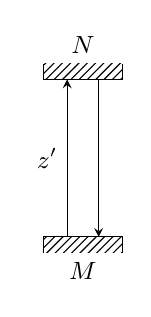
\begin{tikzpicture}
    \draw[pattern=north east lines] (-0.5,2.2)--++(0,-0.2)--++(1,0)--++(0,0.2);
    \draw[pattern=north east lines] (-0.5,-0.2)--++(0,0.2)--++(1,0)--++(0,-0.2);
    \draw (0,-0.2) node [anchor=north]{\small $M$};
    \draw (0,2.2) node [anchor=south]{\small $N$};
    \draw[->,>=stealth] (-0.2,0)--(-0.2,2);
    \draw[<-,>=stealth] (0.2,0)--(0.2,2);
    \draw (-0.2,1) node [anchor=east]{\small $z'$};
  \end{tikzpicture}
  \qquad
  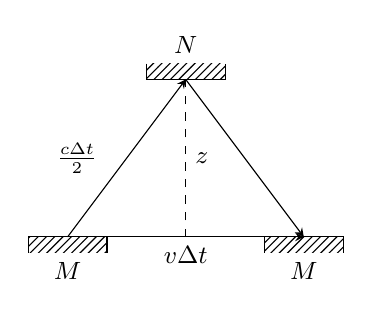
\begin{tikzpicture}
    \draw[pattern=north east lines] (-2,-0.2)--++(0,0.2)--++(1,0)--++(0,-0.2);
    \draw[pattern=north east lines] (1,-0.2)--++(0,0.2)--++(1,0)--++(0,-0.2);
    \draw[pattern=north east lines] (-0.5,2.2)--++(0,-0.2)--++(1,0)--++(0,0.2);
    \draw[->,>=stealth] (-1.5,0)--(0,2);
    \draw[<-,>=stealth] (1.5,0)--(0,2);
    \draw[->,>=stealth] (-1.5,0)--(1.5,0);
    \draw[dashed](0,0)--(0,2);
    \draw (-1,1) node [anchor=east] {\small $\frac{c\Delta t}{2}$};
    \draw (0,0) node [anchor=north]{\small $v\Delta t$};
    \draw (-1.5,-0.2) node [anchor=north]{\small $M$};
    \draw (1.5,-0.2) node [anchor=north]{\small $M$};
    \draw (0,2.2) node [anchor=south]{\small $N$};
    \draw (0,1) node [anchor=west]{\small $z$};
  \end{tikzpicture}
  \caption{垂直分量不变}
  \label{fig:lorentz0}
\end{figure}

考虑光从$M$发出事件到从$N$反回最后再从$M$接收事件.则图\ref{fig:lorentz0}所示左侧为和$M$因联的惯性系中观察到的现象.则
\begin{equation}
  s'^2=c^2(\Delta t')^2=4z'^2
  \label{eq:lorentz0}
\end{equation}
在$O$惯性系中,有
\begin{equation}
  s^2=c^2(\Delta t)^2 -v^2(\Delta t)^2=4z^2
  \label{eq:lorentz1}
\end{equation}
由间隔不变原理,据式\eqref{eq:lorentz0}和式\eqref{eq:lorentz1}可得
\begin{equation}
  z'=z
  \label{eq:lorentz2}
\end{equation}
即:与运动方向垂直的分量不发生变化.

\subsection{方案一}

将洛仑兹变换写为
\begin{gather}
  \left\{
    \begin{gathered}
      x'=a_{11}x+a_{12}ct\\
      ct'=a_{21}x+a_{22}ct
    \end{gathered}
  \right.
\end{gather}
  计算间隔
\begin{align}
  s^2&=c^2t'^2-x'^2\notag\\
  &=(a_{22}^2-a_{12}^2)c^2t^2-(a_{11}^2-a_{12}^2)x^2\notag\\
  &+2(a_{21}a_{22}-a_{11}a_{12})ct\cdot x
\end{align}
于是间隔不变性要求:
\begin{gather}
  \left\{
    \begin{gathered}
      a_{22}^2-a_{12}^2=1\\ 
      a_{11}^2-a_{21}^2=1\\ 
      a_{21}a_{22}-a_{11}a_{12}=0
    \end{gathered}
  \right.
  \label{eq:lorentz3}
\end{gather}
由式\eqref{eq:lorentz3}可得
\begin{equation}
  \frac{a_{21}}{a_{11}}=\frac{a_{12}}{a_{22}}
  \label{eq:lorentz4}
\end{equation}
同时,由于当速度远小于光速时相对论应当回归到经典力学,所以可以判断$a_{11}>0$和$a_{22}>0$,则
\begin{equation}
  a_{11}=\sqrt{1+a_{12}^2}\qquad a_{22}=\sqrt{1+a_{12}^2}
  \label{eq:lorentz5}
\end{equation}
由式\eqref{eq:lorentz4}和式\eqref{eq:lorentz5}对比可得:$a_{12}=a_{21}$.在$O$系中追踪$O'$的运动,则
\begin{gather}
  0=a_{11}vt+a_{12}ct\notag\\
  \intertext{推出}
  \frac{a_{12}}{a_{11}}=-\frac{v}{c}\notag
  \intertext{代入式\eqref{eq:lorentz5}得}
  \left\{
    \begin{gathered}
      a_{11}=\frac{1}{\sqrt{1-\frac{v^2}{c^2}}}\\
      a_{12}=\frac{-v/c}{\sqrt{1-\frac{v^2}{c^2}}}\\
    \end{gathered}
  \right.
  \intertext{于是得到洛仑兹变换}
  \left\{
    \begin{gathered}
      x'=\frac{x-vt}{\sqrt{1-\frac{v^2}{c^2}}}\\
      t'=\frac{t-\frac{v}{c^2}x}{\sqrt{1-\frac{v^2}{c^2}}}
    \end{gathered}
  \right.
\end{gather}

\subsection{方案二}

此推证方法源于一次在期中考试监考过程中偶然想到的.将洛仑兹变换写为

\begin{gather}
  \left\{
    \begin{gathered}
      x'=a_{11}x+a_{12}ct\\
      ct'=a_{21}x+a_{22}ct
    \end{gathered}
  \right.
\end{gather}
追踪$O'$相对于$O$的运动,则
\begin{gather}
  0=a_{11}vt+a_{12}ct
  \intertext{解得}
  \frac{a_{12}}{a_{11}}=-\frac{v}{c}
\end{gather}
将上式代入洛仑兹变换第一式,得
\begin{equation}
  x'=a_{11}(x-vt)
  \label{eq:lorentz6}
\end{equation}
基于相对性原理,可得逆变换
\begin{equation}
  x=a_{11}(x'+vt')
  \label{eq:lorentz7}
\end{equation}
由式\eqref{eq:lorentz6}考虑光传播这一事实,则
\begin{gather}
  ct'=a_{11}(c-v)t
  \intertext{解得}
  \frac{t'}{t}=a_{11}(1-\frac{v}{c})
  \label{eq:lorentz8}
\end{gather}
同理,由式\eqref{eq:lorentz7}考虑光传播这一事实,则
\begin{gather}
  ct=a_{11}(c+v)t'
  \intertext{解得}
  \frac{t'}{t}=\frac{1}{a_{11}}{1+\frac{v}{c}}
  \label{eq:lorentz9}
\end{gather}
式\eqref{eq:lorentz8}和式\eqref{eq:lorentz9}相等,则
\begin{gather}
  a_{11}(1-\frac{v}{c})=\frac{1}{a_{11}(1+\frac{v}{c})}
  \intertext{解得}
  a_{11}=\frac{1}{\sqrt{1-\frac{v^2}{c^2}}}
  \label{eq:lorentz10}
\end{gather}
将式\eqref{eq:lorentz10}代入式\eqref{eq:lorentz6}和式\eqref{eq:lorentz7}联立二式得洛仑兹变换为
\begin{gather}
  \left\{
    \begin{gathered}
      x'=\frac{x-vt}{\sqrt{1-\frac{v^2}{c^2}}}\\
      t'=\frac{t-\frac{v}{c^2}x}{\sqrt{1-\frac{v^2}{c^2}}}
    \end{gathered}
  \right.
\end{gather}

\subsection{方案三}

此法源自于朗道的《场论》 \S4 .二事件的间隔可以认为是在四维空间内的相对应的世界点的距离.所求变换要对距离保持不变,所以在数学上对应四维坐标(ct,x,y,z)的转动.四维空间内的一切转动可以化为六个分别在平面 xy,zy,xz,tx,ty,tz内的转动,考虑到一个特例---在tx平面内的转动.则需借助双曲函数完成,已知双曲函数满足关系
\begin{gather}
\cosh^2\theta-\sinh^2\theta=1
\intertext{所以tx平面内的转动为}
 \left\{
   \begin{gathered}
    x=x'\cosh\theta +ct'\sinh\theta\\
    ct=x'\sinh\theta+ct'\cosh\theta
   \end{gathered}
 \right.
 \label{eq:lorentz11}
\intertext{追踪$O'$在$O$系中的运动,$x'=0$则}
 \left\{
   \begin{gathered}
    vt=ct'\sinh\theta\\
    ct=ct'\cosh\theta
   \end{gathered}
 \right.
 \intertext{解得}
 \tanh\theta=\frac{v}{c}
 \intertext{由于$\cosh\theta>0$所以有}
 \left\{
   \begin{gathered}
     \cosh\theta=\frac{1}{\sqrt{1-\tanh^2\theta}}=\frac{1}{\sqrt{1-\frac{v^2}{c^2}}}\\
     \sinh\theta=\cosh\theta\tanh\theta=\frac{\frac{v}{c}}{\sqrt{1-\frac{v^2}{c^2}}}
   \end{gathered}
 \right.
 \label{eq:lorentz12}
 \intertext{式\eqref{eq:lorentz12}代入式\eqref{eq:lorentz11}得洛仑兹变换}
 \left\{
   \begin{gathered}
     x=\frac{x'+vt'}{\sqrt{1-\frac{v^2}{c^2}}}\\
     t=\frac{t'+\frac{v}{c^2}x'}{\sqrt{1-\frac{v^2}{c^2}}}
   \end{gathered}
 \right.
   \qquad
 \left\{
   \begin{gathered}
     x'=\frac{x-vt}{\sqrt{1-\frac{v^2}{c^2}}}\\
     t'=\frac{t-\frac{v}{c^2}x}{\sqrt{1-\frac{v^2}{c^2}}}
   \end{gathered}
 \right.
 \label{eq:lorentz13}
\end{gather}

\section{固有时}

对比洛仑兹变换和伽利略变换,则它们有很大的不同.原因在于伽利略变换默认的是信号速度是无限大的,所以当物体的速度远小于光速时洛仑兹变换将退回到伽利略变换.这个变化将导致描述物体的运动时对于时间和空间的记录问题,有相应的变更.在伽利略变换中,由于时间是绝对的,它不依赖于任何参考系.所以在经典力学中,记录时间可以在任何位置的时钟上读出数值.但是在相对论中这样做是不行的!我们可以看到,对于一个运动的物体,使其本身携带一个时钟,则可以在这个时钟确定此物体经历的时间.下面来详细讨论这个描述运动的计时问题.

在惯性系$O$中,我们固定在原点$O$上一时钟,当物体在原点时我们可以由此读出时刻.当物体运动另一点时再来读取这个时钟所指示的时刻时就有问题,由于信号速度是有限的,当光由原点传到物体所在地点时物体将会发生运动而到达了另一个位置.所以这是不可行.处理这个问题的关键是在任何一个地点处放置一个与原点的钟对过时的钟,当物体来到此处时就在此处读取时钟的时刻,则这个时刻就是原点处时钟所指示的读数.由于相对论效应,又产生了如何对准时钟的问题.由于当物体运动的速度远小于光速时,坐标间的变换将回到伽利略变换,则时间将变成绝对的.所以可以首先将所有的完全相同的时钟放置在原点$O$处,对齐示数,然后以无限缓慢的速度移动到空间的每一个位置上.这样在空间的每一点上就有一个和原点指示计数相同的钟.这样我们就和经典的情况不相矛盾了,当物体由$A$移动到$B$时,分别从$A$和$B$读取时刻,相减后得到经历的时间.由于各个时钟是和原点时钟对过时的,所以\CJKunderwave{可以认为运动所需要的时间就是原点时钟所指示的时间},只是读取方式上的不同而己.在运动的参考系$O'$原点处也固定一个时钟,由于它在运动,所以它指示的时间和$O$系中是不一样的,但是在$O'$系中,我们也用同样的方法在每一点安放了时钟的,它们所指示的时间和$O'$处的钟示数是相同的.

由上述讨论可知,每一个惯性系,其原点处的时钟决定了整个坐标系的时间问题.因此,原点处的钟指示的时刻我们称为固有时.一个运动的物体,在原点$O'$的钟指示的数值就是此参考系的固有时.

下面我们来讨论$O$系和$O'$中的固有时的关系. 和$O'$中任一位置$x'$固定的时钟,它指示的时间总是在$x'$时的值,但是由于在$O$看来,$O'$是运动的,则在$O$中经历的时间将是由$O$中不同的位置(即$O'$)所在处的时钟指示的时刻计算出来的,由于对过时,所以它也就是$O$处不动时钟的示数.基于这个关系,考虑洛仑兹变换式
\begin{gather}
  \left\{
    \begin{gathered}
      t_1=\frac{t_1'+\frac{v}{c^2}x'}{\sqrt{1-\frac{v^2}{c^2}}}\\
      t_2=\frac{t_2'+\frac{v}{c^2}x'}{\sqrt{1-\frac{v^2}{c^2}}}
    \end{gathered}
  \right.
  \label{eq:guyoushi0}
  \intertext{注意$x_1\neq x_2$ ,所以令二者相减得}
  \Delta t =\frac{\Delta t'}{\sqrt{1-\frac{v^2}{c^2}}}
\end{gather}
由上述讨论可得$\Delta t >\Delta t'$ 即一物体运动起来后,其上的固有时$\Delta t'$和其静止于$O$系时的固有时$\Delta t$ 相比变小了,即运动物体的时钟变慢了!

讨论完时间,我们再来讨论一下距离.当一个刚性杆,注意是刚性的!它不能发生实质性的变形.在此杆在$O$中沿$x$轴匀速直线运动时,我们要测量它的长度,必须在同一时刻测定!这可以通过在杆的两端上放上两个人在同一时刻$t$读取在$O$中的坐标,然后相减我们就得到了它的长度.但是在和杆固连的$O'$系中,由于杆是静止的,所以测量它两端的坐标不受时间限制,所以在$O'$中测量杆的长度时,可以先在$t'_1$时读取$A$端坐标$x'_A$,然后跑到另一端,时间必定不与之相同了,即在$t'_2$时刻读取$B$端坐标$x'_B$,则在$O'$中杆的长度为$\Delta x'=x'_B-x'_A$.由于在$O'$中讨论杆的长度对时刻没有限制,所以考虑逆洛仑兹变换式
\begin{gather}
  \left\{
    \begin{gathered}
      x'_1=\frac{x_1-vt}{\sqrt{1-\frac{v^2}{c^2}}}\\
      x'_2=\frac{x_2-vt}{\sqrt{1-\frac{v^2}{c^2}}}
    \end{gathered}
  \right.
  \label{eq:guyoushi1}
  \intertext{注意$t'_1\neq t'_2$ ,所以令二者相减得}
  \Delta x'=\frac{\Delta x}{\sqrt{1-\frac{v^2}{c^2}}}
  \intertext{简单计算可得}
  \Delta x=\Delta x'\cdot\sqrt{1-\frac{v^2}{c^2}}
\end{gather}
由上述可得,一个不可伸缩的刚性杆,由于相对论效应会导致在标静止时的长度和运动起来时的长度有所不同.即在$O$系中测得运动杆长$\Delta x$和$O'$系中测得的静止杆长$\Delta x'$相比要小!即运动的刚性杆变短了!


\section{相对论的速度变换}

如果一个物体在$O$和$O'$中都是运动的,则它们的速度变换关系叫做相对论的速度变换.借助洛仑兹变换不难得到这一变换.
\begin{gather}
 \left\{
   \begin{gathered}
     t=\frac{t'+\frac{v}{c^2}x'}{\sqrt{1-\frac{v^2}{c^2}}}\\
     x=\frac{x'+vt'}{\sqrt{1-\frac{v^2}{c^2}}}\\
     y=y'\\
     z=z'
   \end{gathered}
 \right.
 \label{eq:vtransform0}
 \intertext{分别取微小变量,得}
 \left\{
   \begin{gathered}
     \Delta t=\frac{1+\frac{vu'_x}{c^2}}{\sqrt{1-\frac{v^2}{c^2}}}\Delta t'\\
     \Delta x=\frac{u'_x+v}{\sqrt{1-\frac{v^2}{c^2}}}\Delta t'\\
     \Delta y =\Delta y'\\
     \Delta z=\Delta z'
   \end{gathered}
 \right.
 \label{eq:vtransform1}
 \intertext{令式\eqref{eq:vtransform1}中后三式除以第一式的时间,可得}
 \left\{
   \begin{gathered}
     u_x=\frac{u'_x+v}{1+\frac{vu'_x}{c^2}}\\
     u_y=\frac{u'_y\sqrt{1-\frac{v^2}{c^2}}}{1+\frac{u'_xv}{c^2}}\\
     u_z=\frac{u'_z\sqrt{1-\frac{v^2}{c^2}}}{1+\frac{u'_xv}{c^2}}
   \end{gathered}
 \right.
\end{gather}

\section{相对论中的力学量}

\subsection{自由粒子的拉格朗日函数}

自由粒子在惯性系中做匀速直线运动.同时由欧几里德几何可知三维空间中两点间直线最短,所以对于四维空间中的间隔就对应有一个结论,从一个世界点到另一个世界点,积分$\int \mathrm{d}s$沿直世界线进行时,具有最大值.原因在于,对于两个确定的世界点,则它们之间的时间是确定的,但是三维空间中的路径可以有多种,而当路径为直线时$r^2$最小,由间隔的定义$s^2=c^2t^2-r^2$可得,当路径为直线时间隔是最大的.对于一个自由粒子而言,它的实际路径就是直线,所以其沿世界线的积分$\int \mathrm{d}s$将具备最大值.

按照分析力学中的最小作用原理,主函数的变分具有最小值.综合自由粒子沿世界线的积分最大,而主函数又是一个标量所以其应当为洛仑兹不变量,同时在洛仑兹变换中又有间隔不变原理,据此可以推断出自由粒子主函数一定具备如下形式
\begin{equation}
  S=-\alpha \int \mathrm{d}s
  \label{eq:zhuhanshuS}
\end{equation}
式中$\alpha$是一个大于零的实数.下面来确定常数$\alpha$的值,将间隔用固有时表出,则
\begin{equation}
  S=-\alpha c \int \mathrm{d}\tau =-\alpha c \int \sqrt{1-\frac{v^2}{c^2}} \mathrm{d}t
  \label{eq:zhuhanshuS0}
\end{equation}
式\eqref{eq:zhuhanshuS0}和主函数的定义对比可得拉格朗日函数为
\begin{equation}
  L=-\alpha c \sqrt{1-\frac{v^2}{c^2}}
  \label{eq:zhuhanshuS1}
\end{equation}
当$v \ll c$时,相对论的公式应当回归到经典情况,将式\eqref{eq:zhuhanshuS1}Taylor 展开,然后取$v^2$项得
\begin{equation}
  L=-\alpha c -\frac{1}{2}\alpha \frac{v^2}{c}
  \label{eq:zhuhanshuS2}
\end{equation}
同时经典的情况为
\begin{equation}
  L=\frac{1}{2}mv^2
  \label{eq:zhuhanshuS3}
\end{equation}
由于在拉格朗日函数中多一个常数不会有任何影响,所以对比式\eqref{eq:zhuhanshuS2}和式\eqref{eq:zhuhanshuS3}可得常数$\alpha =  mc$.于是相对论中的拉格朗日函数为
\begin{equation}
  L=-mc^2\sqrt{1-\frac{v^2}{c^2}}
  \label{eq:zhuhanshuS4}
\end{equation}
由分析力学可知
\begin{equation}
  p_i =-\frac{\partial S}{\partial x^i}=\frac{\partial L}{\partial v^i}
  \label{eq:zhuhanshuS5}
\end{equation}
由于主函数作为一个标量,其梯度是一个洛仑兹协变矢量,所以可以由式\eqref{eq:zhuhanshuS5}求出四维动量(其满足洛仑兹协变性)为
\begin{equation}
  p_i=\left (\frac{E}{c},-\frac{m\vec{v}}{\sqrt{1-\frac{v^2}{c^2}}}\right )
  \label{eq:zhuhanshuS6}
\end{equation}
所以可得在相对论中的动量表达式为
\begin{equation}
  \vec{p}=\frac{m\vec{v}}{\sqrt{1-\frac{v^2}{c^2}}}
  \label{eq:zhuhanshuS10}
\end{equation}
显然当$v\ll c$时,式\eqref{eq:zhuhanshuS10}回归到经典公式$\vec{p}=m\vec{v}$.同理可以得到四维动量的逆变形式为
\begin{equation}
  p^i=\left (\frac{E}{c},\frac{m\vec{v}}{\sqrt{1-\frac{v^2}{c^2}}}\right )
  =\left(\frac{E}{c},\vec{p}\right)
  \label{eq:zhuhanshuS11}
\end{equation}
考虑到动量与速度的经典关系,所以可以得出四维速度的表达式(此处兼顾了朗道书的定义)
\begin{equation}
  u^i=\frac{p^i}{mc}=\left(\frac{E}{mc^2},\frac{\vec{v}}{c\sqrt{1-\frac{v^2}{c^2}}}\right)
  \label{eq:zhuhanshuS12}
\end{equation}
在式\eqref{eq:zhuhanshuS12}中的速度部分,显然其是坐标对间隔的微分,即
\begin{equation}
  \frac{\mathrm{d}\vec{r}}{\mathrm{d}s}=\frac{\vec{v}}{c\sqrt{1-\frac{v^2}{c^2}}}
  \label{eq:zhuhanshuS13}
\end{equation}
而四维坐标的表达式为
\begin{equation}
  x^i=\left( ct,\vec{r}\right)
  \label{eq:zhuhanshuS14}
\end{equation}
四维坐标是协变矢量,间隔为洛仑兹不变量,所以一个协变矢量对一个洛仑兹不变量微分也将获得一个洛仑兹矢量.即
\begin{equation}
  u^i=\frac{\mathrm{d}x^i}{\mathrm{d}s}=\left(\frac{1}{\sqrt{1-\frac{v^2}{c^2}}},\frac{\vec{v}}{c\sqrt{1-\frac{v^2}{c^2}}}\right)
  \label{eq:zhuhanshuS15}
\end{equation}
对照式\eqref{eq:zhuhanshuS15}和式\eqref{eq:zhuhanshuS12}的第零分量,可得相对论下自由粒子的能量为
\begin{equation}
  E=\frac{mc^2}{\sqrt{1-\frac{v^2}{c^2}}}
  \label{eq:zhuhanshuS16}
\end{equation}
于是四维动量又可以写作
\begin{equation}
  p^i=\left (\frac{mc}{\sqrt{1-\frac{v^2}{c^2}}},\frac{m\vec{v}}{\sqrt{1-\frac{v^2}{c^2}}}\right )
  \label{eq:zhuhanshuS17}
\end{equation}
由内积的变换不变性,考虑式\eqref{eq:zhuhanshuS11}和式\eqref{eq:zhuhanshuS17},由于变换不变性,则在式\eqref{eq:zhuhanshuS17}中取$v=0$也不影响内积,则可得能量与动量的相对论关系为
\begin{gather}
  p^ip_i=\frac{E^2}{c^2}-p^2=m^2c^2
  \intertext{所以相对论能量与动量的关系为}
  \frac{E^2}{c^2}=p^2+m^2c^2
  \label{eq:zhuhanshuS18}
\end{gather}
由四维动量的定义,同时考虑内积的洛仑兹不变性可得
\begin{gather}
  p^ip_i=m^2c^2
  \intertext{上式对间隔微分可得}
  p^i\frac{\mathrm{d}p_i}{\mathrm{d}s}=0
  \intertext{经过简单计算得}
  \frac{mc}{\sqrt{1-\frac{v^2}{c^2}}}\cdot\frac{\mathrm{d}p^0}{\mathrm{d}{s}}
  -\frac{m\vec{v}\cdot\vec{f}}{c(1-\frac{v^2}{c^2})}=0
  \intertext{由此可以方便得到动量第零分量对间隔的微分}
  \frac{\mathrm{d}p^0}{\mathrm{d}s}
  =\frac{\vec{f}\cdot\vec{v}}{c^2\sqrt{1-\frac{v^2}{c^2}}}
  \intertext{于是得四维力为}
  g^i=\frac{\mathrm{d}p^i}{\mathrm{d}s}=
  \left(
    \frac{\vec{f}\cdot\vec{v}}{c^2\sqrt{1-\frac{v^2}{c^2}}},
  \frac{\vec{f}}{c\sqrt{1-\frac{v^2}{c^2}}}
  \right)
\end{gather}
上式中力$\vec{f}=\frac{\mathrm{d}\vec{p}}{\mathrm{d}t}$,仍然是动量对时间的导数.

\subsection{再议速度变换公式}

上一节定出了四维速度的形式,在$O$系中即
\begin{equation}
  u^i=\frac{\mathrm{d}}{\mathrm{d}s}\left(ct,\vec{r}\right)
  \label{eq:4weiV}
\end{equation}
上述间隔在随物体一块运动的参考系中表出,同时为了书写简洁选择速度单位为光速$c$,则
\begin{equation}
  u^i=\left(\frac{1}{\sqrt{1-u_x^2}},\frac{\vec{u}}{\sqrt{1-u_x^2}}\right)
  \label{eq:4weiV0}
\end{equation}
同理在$O'$系中表出物体的四维坐标,除以该物体在随其自身一同运动的参考系中的间隔表达式,则
\begin{equation}
  u'^i=\left(\frac{1}{\sqrt{1-u^{\prime 2}}_x},\frac{\vec{u}'}{\sqrt{1-u^{\prime 2}_x}}\right)
  \label{eq:4weiV1}
\end{equation}
四维速度满足洛仑兹变换,注意在洛仑兹变换中的速度$v$是$O'$相对于$O$运动的速度.则
\begin{gather}
  \left\{
    \begin{gathered}
      \frac{u_x}{\sqrt{1-u_x^2}}=\frac{u'_x+v}{\sqrt{1-u^{\prime 2}_x}\sqrt{1-v^2}}\\ 
      \frac{u_y}{\sqrt{1-u_x^2}}=\frac{u_y'}{\sqrt{1-u^{\prime 2}_x}}\\
      \frac{u_z}{\sqrt{1-u_x^2}}=\frac{u_z'}{\sqrt{1-u^{\prime 2}_x}}\\
      \frac{1}{\sqrt{1-u_x^2}}=\frac{1+u'_xv}{\sqrt{1-u^{\prime 2}_x}\sqrt{1-v^2}}
    \end{gathered}
  \right.
  \label{eq:4weiV2}
  \intertext{由式\eqref{eq:4weiV1}中前三式分另除以第四式可得速度变换关系为}
  \left\{
    \begin{gathered}
      u_x=\frac{u'_x+v}{1+u'_xv}\\
      u_y=\frac{u'_y\sqrt{1-v^2}}{1+u'_xv}\\
      u_z=\frac{u'_z\sqrt{1-v^2}}{1+u'_xv}
    \end{gathered}
  \right.
  \label{eq:4weiV3}
  \intertext{如果恢复为国际单位,则式\eqref{eq:4weiV3}化为}
 \left\{
   \begin{gathered}
     u_x=\frac{u'_x+v}{1+\frac{vu'_x}{c^2}}\\
     u_y=\frac{u'_y\sqrt{1-\frac{v^2}{c^2}}}{1+\frac{u'_xv}{c^2}}\\
     u_z=\frac{u'_z\sqrt{1-\frac{v^2}{c^2}}}{1+\frac{u'_xv}{c^2}}
   \end{gathered}
 \right.
\end{gather}

\section{相对速度}

\subsection{不变量标量计算法}

在$O$系中有两个物体1和2,其速度分别为$\vec{v}_1$和$\vec{v}_2$,考虑内积的洛仑兹不变性,为了方便书写,以光速$c$作为速度的单位,则相当于所有公式中令$c=1$即可,于是
\begin{gather}
  p_{1i}p^{2i}=\frac{m_1m_2}{\sqrt{1-v^2}}
  \label{eq:xiangduiV}
  \intertext{上式右式是在认为2的速度为零时的相对坐标系中写出的,左式在$O$系中写出,则}
  \frac{m_1m_2}{\sqrt{(1-v_1^2)(1-v_2^2)}}-m_1m_2v_1v_2\cos\theta=\frac{m_1m_2}{\sqrt{1-v^2}}
  \intertext{上式约去$m_1m_2$,经过简单计算可得}
  v=\frac{\sqrt{v_1^2+v_2^2-2v_1v_2\cos\theta +v_1^2v_2^2\sin^2\theta}}{1-v_1v_2\cos\theta}
  \intertext{上式也可以写为更加简洁的矢量式}
  v=\frac{\sqrt{(\vec{v}_1-\vec{v}_2)^2-(\vec{v}_1\times\vec{v}_2)^2}}{1-\vec{v}_1\cdot\vec{v}_2}
\end{gather}
显然,当物体的速度远小于光速时,即$v_1\ll 1,v_2\ll 1$时,上式化经典情况
\begin{equation}
  v=\left|\vec{v}_1-\vec{v}_2\right|
  \label{eq:xiangduiV0}
\end{equation}

\subsection{矢量计算法}

在$O_0$中物体1和2的速度分别为$\vec{v}_1$和$\vec{v}_2$,此处隐含着还有一个物体参与运动,也就是参考系$O_0$,要求出2相对于1的相对速度,必须假定1不动,此时需确定$O_0$相对于1的速度也就是$-\vec{v}_1$.而此时2相对于$O_0$的速度还是$\vec{v}_2$,实际上这里的问题转化为三步:第一步,求出$O_0$相对于1的速度,而1变成了参考系$O$,原来的$O_0$变成了$O'$.第二步,物体2相对于$O_0$的运动,现在变成是在新的$O'$中的运动,其速度仍然为$\vec{v}_2$.第三步,由洛仑兹变换求出新$O$系中物体2的速度,也就是2相对于1的速度了.

为了讨论问题的方便仍然取速度单位为光速,同时取$\vec{v}_1$方向为$x$轴.则$O'$相对于$O$的速度为$-v_1$,由洛仑兹变换得2相对于1的速度$\vec{v}$为
\begin{gather}
\left\{
  \begin{gathered}
    v_x=\frac{v_{2x}-v_1}{1-v_{2x}v_1}\\
    v_y=\frac{v_y\sqrt{1-v_1^2}}{1-v_{2x}v_1}\\
    v_z=\frac{v_z\sqrt{1-v_1^2}}{1-v_{2x}v_1}
  \end{gathered}
\right.
\end{gather}
下面求相对速度的大小
\begin{align}
  v&=\sqrt{v_x^2+v_y^2+v_z^2}\notag\\
  &=\frac{\sqrt{(v_{2x}-v_1)^2+v_{2y}^2(1-v_1^2)+v_{2z}^2(1-v_1)^2}}{1-v_{2x}v_1}\notag\\
  &=\frac{\sqrt{v_1^2+v_2^2-2v_{2x}v_1-(v_{2y}^2+v_{2z}^2)v_1^2}}{1-v_{2x}v_1}\notag
  \intertext{上式可以写成矢量式,如此则与所确定的坐标轴指向就没有特定的关系了,于是得}
  &=\frac{\sqrt{(\vec{v}_1-\vec{v}_2)^2-(\vec{v}_1\times\vec{v}_2)^2}}{1-\vec{v}_1\cdot\vec{v}_2}
  \label{eq:xiangduiV1}
\end{align}

\section{分布函数的变化}

\subsection{基本数学原理}

在这一节谈到了动量``体积元''的变换,用到了超曲面等概念,我对此并不是很熟悉,所以在此消耗了较长的时间来说明这一问题.考虑一个n+1维矢量
\begin{equation}
  A=(a_1,a_2,\cdots,a_{n+1})
\end{equation}
我们来确定与A垂直的n+1维矢量的最大个数,以$B_i$表示第$i$个与A垂直的矢量.则这个问题转化为了下列方程组最多有几个非零解的问题.按照克莱姆法则求线性代数解的方法易知,与A垂直的n+1维向量最多只能有n个,即
\begin{gather}
  \left\{
    \begin{gathered}
      a_1b_{11}+a_2b_{12}+\cdots a_{n+1}b_{1,n+1}=0\notag\\
      a_1b_{21}+a_2b_{22}+\cdots a_{n+1}b_{2,n+1}=0\notag\\
      \cdots  \notag\\
      a_1b_{n1}+a_2b_{n2}+\cdots a_{n+1}b_{n,n+1}=0\notag
    \end{gathered}
  \right.
  \label{eq:NweiS0}
\end{gather}
同时按照行列式的计算规则,如果有两行(或两列)相同,则行列式的值为零.以$\vec{e}_i$表示n+1维向量的各个基,也就是说A的实体表示为
\begin{equation}
  A=a_1\vec{e}_1+a_2\vec{e}_2+\cdots+a_{n+1}\vec{e}_{n+1}
  \label{eq:NweiS1}
\end{equation}
如下用实体基构建行列式
\begin{equation}
  C=
  \begin{vmatrix}
    \vec{e}_1&\vec{e}_2&\vec{e}_3&\cdots&\vec{e}_{n+1}\\
    b_{11}&b_{12}&b_{13}&\cdots&b_{1,n+1}\\
    b_{21}&b_{22}&b_{23}&\cdots&b_{2,n+1}\\
    &&\vdots&&\\
    b_{n1}&b_{n2}&b_{n3}&\cdots&b_{n,n+1}
  \end{vmatrix}
\end{equation}
显然考虑$B_i$与C的内积,相当于以第i个B矢量的各个分量分别取代C第一行的n+1个基,原因是n+1个基是相互正交的.显然B的这n个矢量都与C垂直.同时在n+1维空间内与C垂直的矢量必然都线性相关.于是可得C与A是线性相关的.设比例系数为$\lambda$,下面我们来说明在线性变换下此系数是不变的.设变换矩阵为D,则
\begin{gather}
  C=\lambda A
  \intertext{以D分别左作用上式得}
  CD=\lambda AD
  \intertext{由于$C'=CD$,$A'=AD$,所以在新的基底下有}
  C'=\lambda A' 
\end{gather}
这就说明了,如果两个高维向量线性相关,则在线性变换它们的比例系数是不变的.同时,因为比例系数是一个标量,所以它是不变的也不难理解.

\subsection{动量微元的变换}

在相对论中动量的内积是一个洛仑兹不变量.于是我们可以得到一个垂直关系,即
\begin{gather}
  p^ip_i=m^2c^2
  \intertext{对上式取变分,则}
  p^i\delta p_i=0
\end{gather}
$p^i$是一个四维矢量,所以能够找到的线性无关的与$p^i$垂直的三个四维矢量.一个最简单的取法是当取$\mathrm{d}p_x$时,其余动量变化都是零,但是能量会有相应的变化,于是这样的三个四维矢量分别可以取为
\begin{gather}
  \left\{
    \begin{gathered}
      \left(\mathrm{d}E_1,\mathrm{d}p_x,0,0\right)\\ 
      \left(\mathrm{d}E_1,0,\mathrm{d}p_y,0\right)\\ 
      \left(\mathrm{d}E_1,0,0,\mathrm{d}p_z\right)
    \end{gathered}
  \right.
\end{gather}
于是考虑由这三个矢量构成的外积,则必然与四维矢量$p^i$线性相关,则比例系数是一个洛仑兹不变量.即这个外积是
\begin{equation}
  \begin{vmatrix}
    \vec{e}_0 & \vec{e}_1&\vec{e}_2&\vec{e}_3\\
    \mathrm{d}E_1&\mathrm{d}p_x&0&0\\
    \mathrm{d}E_2&0&\mathrm{d}p_y&0\\
    \mathrm{d}E_3&0&0&\mathrm{d}p_z
  \end{vmatrix}
  \label{eq:dongliangP}
\end{equation}
显然外积第零分量为$\mathrm{d}p_x\mathrm{d}p_y\mathrm{d}p_z$,四维动量$p^i$的第零分量为$E$,所以其比例系数$\lambda$为
\begin{equation}
  \lambda =\frac{\mathrm{d}p_x\mathrm{d}p_y\mathrm{d}p_z}{E}
  \label{eq:dongliangP1}
\end{equation}
根据前述的高维微量分析可知,在洛仑兹变换过程中比例系数是不发生变化的.

粒子数$f\mathrm{d}p_x\mathrm{d}p_y\mathrm{d}p_z$是一个标量,显然它不应当随参考系的变换而发生变化,将其写为
\begin{equation}
  f(\vec{p})\mathrm{d}p_x\mathrm{d}p_y\mathrm{d}p_z
  =
  f(\vec{p})E\frac{\mathrm{d}p_x\mathrm{d}p_y\mathrm{d}p_z}{E}
  \label{eq:dongliangP2}
\end{equation}
则分布函数与能量的乘积是一个不变量.则
\begin{equation}
  f(\vec{p})E=f(\vec{p}^{\ \prime})E'
  \label{eq:dongliangP3}
\end{equation}

同时由于动量和能量的关系$E^2=p^2+m^2$,所以可得$p\mathrm{d}p=E\mathrm{d}E$,于是将动量微元写成球坐标的形式,得
\begin{equation}
  \frac{\mathrm{d}p_x\mathrm{d}p_y\mathrm{d}p_z}{E}=
  \frac{p^2\mathrm{d}p\mathrm{d}o}{E}=p\mathrm{d}E\mathrm{d}o
  \label{eq:dongliangP4}
\end{equation}
于是又得到一个不变量$p\mathrm{d}E\mathrm{d}o$.对于体积,由洛仑兹变换可得

\begin{gather}
  \mathrm{d}V=\mathrm{d}V_0\sqrt{1-v^2}\qquad
  \mathrm{d}V'=\mathrm{d}V_0\sqrt{1-v^{\prime2}}
  \intertext{所以有}
  \frac{\mathrm{d}V}{\mathrm{d}V'}=
  \frac{\sqrt{1-v^2}}{\sqrt{1-v^{\prime2}}}
  =\frac{E'}{E}
  =\frac{\mathrm{d}p'_x\mathrm{d}p'_y\mathrm{d}p'_z}{\mathrm{d}p_x\mathrm{d}p_y\mathrm{d}p_z}
  \intertext{所以可得}
\mathrm{d}V\mathrm{d}p_x\mathrm{d}p_y\mathrm{d}p_z=
\mathrm{d}V'\mathrm{d}p'_x\mathrm{d}p'_y\mathrm{d}p'_z
\end{gather}
于是可得相空间内的体元$\mathrm{d}\tau$也是一个洛仑兹不变量.同时由于在一个相元内的粒子数$f\mathrm{d}\tau$显然也是一个不变量,所以可得分布函数$f(\vec{r},\vec{p})$也是一个不变量.

\section{粒子的衰变}

这一节的讨论的内容不难,但是在习题中分析衰变后粒子的最大偏角时的计算其实有点麻烦.在这里首先引一个我在高中时期分析出的椭圆计算公式,在此处可以极大的降低计算量.

\subsection{椭圆的解析分析}

如图所示
\begin{figure}[H]
  \centering
  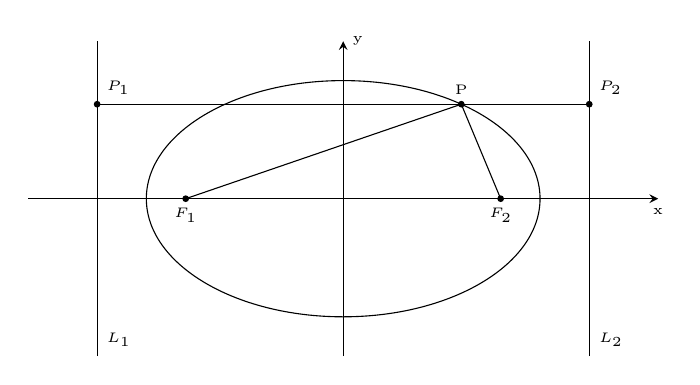
\begin{tikzpicture}
    \draw [->,>=stealth](-4,0)--(4,0) node [anchor=north]{\tiny x};
    \draw [->,>=stealth](0,-2)--(0,2) node [anchor=west]{\tiny y};
    \filldraw (2,0) circle [radius=1pt] node [anchor=north]{\tiny $F_2$};
    \filldraw (-2,0) circle [radius=1pt] node [anchor=north]{\tiny $F_1$};
    \draw(-3.125,-2)--(-3.125,2);
    \draw(3.125,-2)--(3.125,2);
    \draw (0,0) ellipse (2.5 and 1.5);
    \draw (-2,0)--(1.5,1.2)--(2,0);
    \filldraw (1.5,1.2) circle [radius=1pt] node [anchor=south]{\tiny P};
    \draw (-3.125,1.2)--(3.125,1.2);
    \filldraw (-3.125,1.2) circle [radius=1pt] node [anchor=south west] {\tiny $P_1$};
    \filldraw (3.125,1.2) circle [radius=1pt] node [anchor=south west] {\tiny $P_2$};
    \draw (-3.125,-2)node [anchor=south west] {\tiny $L_1$};
    \draw (3.125,-2)node [anchor=south west] {\tiny $L_2$};
  \end{tikzpicture}
  \caption{椭圆}
  \label{fig:tuoyuan}
\end{figure}

\begin{gather}
  \intertext{椭圆的标准解析方程为} 
  \frac{x^2}{a^2}+\frac{y^2}{b^2}=1
  \label{eq:tuoyuan}
  \intertext{准线方程为}
  \left\{
    \begin{gathered}
      l_1:x_1=-\frac{a^2}{c}\\
      l_2:x_2=\frac{a^2}{c}
    \end{gathered}
  \right.
  \intertext{定和性质:}
  |PF_1|+|PF_2|=2a
  \intertext{定比性质:}
  \frac{|PF_1|}{|PP_1|}=\frac{|PF_2|}{|PP_2|}=e=\frac{c}{a}
  \intertext{e为离心率.过椭圆上一点$(x_0,y_0)$的切线方程:}
  \frac{xx_0}{a^2}+\frac{yy_0}{b^2}=1
  \intertext{记斜率为k,则切线的斜率和切点间的关系为}
  k\cdot\frac{y_0}{x_0}=-\frac{b^2}{a^2}
  \intertext{一般高中常用联立方程的形式求$x_1+x_2$,$y_1+y_2$,$x_1x_2$,$y_1y_2$.高考中数学大题必出此类型,从对称的观点可以证明下式成立.}
  \left\{
    \begin{gathered}
      \frac{x^2}{a^2}+\frac{y^2}{b^2}=1\\
      Ax+By+C=0 
    \end{gathered}
  \right.
  \intertext{由直线解得$y=-\frac{Ax+C}{B}$代入椭圆方程可得}
  (A^2a^2+B^2b^2)x^2+Aa^22Cx+a^2(C^2-B^2b^2)=0
  \intertext{注意上式是极其对称的,为了快速解题,需要同学位根据对称的特点背过.其判别式为}
  \Delta_x=4a^2b^2B^2(A^2a^2+B^2b^2-C^2)
  \intertext{于是判定直线与椭圆有无交点只需判断$A^2a^2+B^2b^2$与$C^2$的大小关系即可.}
  A^2a^2+B^2b^2>C^2
  \intertext{上式成立则有两个交点}
  A^2a^2+B^2b^2=C^2
  \intertext{上式成立则有一个交点}
  A^2a^2+B^2b^2<C^2
  \intertext{上式成立则无交点,同时基于x,y的同等地位和对称性,易写出关于y的联立方程式和判别式}
  \left\{
    \begin{gathered}
      (A^2a^2+B^2b^2)y^2+Bb^22Cy+b^2(C^2-A^2a^2)=0\\
      \Delta_y=4a^2b^2A^2(A^2a^2+B^2b^2-C^2)
    \end{gathered}
  \right.
  \intertext{显然由韦达定理易得$x_1+x_2$,$y_1+y_2$,$x_1x_2$,$y_1y-2$之值,此不再赘述.下面再来看一看弦长的问题.一般的x方程为:}
  (x-x_1)(x-x_2)=0\notag\\
  x^2-(x_1+x_2)x+x_1x_2=0\notag\\
  \Delta_x=(x_1+x_2)^2-4x_1x_2=(x_1-x_2)^2
  \intertext{同理}
  \Delta_y=(y_1-y_2)^2
  \intertext{所以有弦长l为}
  l=\sqrt{(x_1-x_2)^2+(y_1-y_2)^2}=\sqrt{\Delta_x+\Delta_y}\notag
  \intertext{代入$\Delta_x$和$\Delta_y$解得}
  l=\frac{2ab}{A^2a^2+B^2b^2}\sqrt{(A^2+B^2)(A^2a^2+B^2b^2-C^2)}
\end{gather}

\subsection{衰变时粒子的偏角问题}

此问题源于习题的第1题:一个以速度V运动的粒子在``飞行''中分解为两个粒子.求这些粒子的出射角同其能量的能量间的关系.

在此问题中可以认为这个飞行的粒子本来就由两个粒子构成,两个粒子以共同的速度V飞行,在某一时刻分离开来,而具体结节则由二者相互作用决定.取其中一个粒子其在C系中的能量为$E_0$,在L系中能量为$E$,出射角为在L系中观察的,所以由洛仑兹变换得
\begin{equation}
  E_0=\frac{E-Vp\cos\theta}{\sqrt{1-V^2}}
  \label{eq:shuaibian}
\end{equation}
解得
\begin{equation}
  \cos\theta =\frac{E-E_0\sqrt{1-V^2}}{Vp}
  \label{eq:shuaibian0}
\end{equation}
同时考虑到动量和能量关系,则$p=\sqrt{E^2-m^2}$代入上式得
\begin{equation}
  \cos\theta =\frac{E-E_0\sqrt{1-V^2}}{V\sqrt{E^2-m^2}}
  \label{eq:shuaibian1}
\end{equation}

对偏转角的范围在动量变换中分析比较容易.在发生衰变的平面内可以取为xy平面,则衰变前后动量的z分量都为0.在动量中心系C中研究问题较方便,在此系中两个粒子初始都处于静止状态,衰变后则两个以相同动量大小向相反的两个方向飞去(由于动量守恒,则二个粒子动量大小相同),设在C系中加以下标``0'',则由洛仑兹变换得
\begin{gather}
  \left\{
    \begin{gathered}
      p_x=\frac{p_{x0}+E_0V}{\sqrt{1-V^2}}\\
      p_y=p_{y0}
    \end{gathered}
  \right.
\end{gather}
至于在C系中,具体的能量和动量取为何值这取决于衰变的性质,而仅有的数据不能确定.所以写出$p_x,p_y$的关系,得
\begin{gather}
  \frac{\left(p_x-\frac{VE_0}{1-V^2}\right)^2}{\left(p_0/\sqrt{1-V^2}\right)}
  +\frac{p_y^2}{p_0^2}=1
\end{gather}
当$\frac{VE_0}{\sqrt{1-V^2}}<p_0/\sqrt{1-V^2}$时,原点位于椭圆内部,则此时夹角为$\theta$的可能性只有一种.当$\frac{VE_0}{\sqrt{1-V^2}}>p_0/\sqrt{1-V^2}$时,则原点位于椭圆外部,则对应于一个$\theta$角,有两个可能的动量值.但是这个角有一定的限度,当过原点的直线与椭圆相切时此角达到最大.写出直线方程为
\begin{equation}
\tan\theta_m \cdot (p_x-\frac{VE_0}{1-V^2})-p_y+\tan\theta_m\frac{VE_0}{1-V^2}
=0
  \label{eq:shuaibian2}
\end{equation}
由椭圆与直线相切的条件$A^2a^2+B^2b^2=C^2$可得
\begin{gather}
  \tan^2\theta_m\cdot\frac{p_0^2}{1-V^2}+p_0^2=\tan^2\theta_m\cdot\frac{V^2E_0^2}{1-V^2} 
  \intertext{将$E_0^2=p_0^2+m^2$代入上式得}
  \tan^2\theta_m\cdot\frac{p_0^2}{1-V^2}+p_0^2=\tan^2\theta_m\cdot\frac{V^2(p_0^2+m^2)}{1-V^2} 
  \intertext{简单计算可得 }
  \sin\theta_m=\frac{p_0\sqrt{1-V^2}}{mV}
\end{gather}

在{\bf\S13 粒子的弹性碰撞}一节,式13.8也有和此处类似的推证,下面说明之.二个粒子1和2发生弹性碰撞,则L系中始情况为2静止,1以速度$\vec{v_1}$运动.所发生的弹性碰撞过程可以理解为开始二者的动量不同,在相互作用的过程中必然有一个时刻二者以共同的速度运动,由于整个过程中动量守恒所以这个速度就是动量中心系的速度V.下一个时刻二都分离,则1以一定的角度射出,从达到共同速度之后的过程可以等价于一个以速度V运动着的复合粒子发生发衰变.所以这和衰变的分析是相同的.唯一要做的是求出质心速度V.下面的计算中,认为``衰变''过程中分析的是第一个粒子,则
\begin{gather}
  \vec{p}=\vec{p}_1\notag\\
  E=E_1+m_2\notag
  \intertext{所以质心的速度为}
  V=\frac{\vec{p}}{E}=\frac{\vec{p}_1}{E_1+m_2}
\end{gather}
2粒子初始时在L系中静止,所以相对于质心的速度大小也为$V$,于是在C系中2的初始动量为
\begin{equation}
  \frac{m_2V}{\sqrt{1-V^2}}
\end{equation}
由于发生的是弹性碰撞,则在C系来看仅仅是粒子的速度方向发生了变化,其动量大小没有变化.所以``衰变''后2粒子的动量与初始的值大小相同.由于在质心系中总动量为零,所以1在衰变后的动量也与2的动量数值相同.所以得到
\begin{equation}
 p_0=\frac{m_2V}{\sqrt{1-V^2}}
\end{equation}
解得
\begin{equation}
  m_2=\frac{p_0\sqrt{1-V^2}}{V}
  \label{eq:shuaibian3}
\end{equation}
所以存在最大角的条件$\frac{VE_0}{\sqrt{1-V^2}}>p_0/\sqrt{1-V^2}$变为
\begin{gather}
  VE_0>p_0
  \intertext{将能量用1的质量表达出来,$p_0$ 用2的质量表达出来}
  \frac{Vm_1}{\sqrt{1-V^2}}>\frac{m_2V}{\sqrt{1-V^2}}
  \intertext{即}
  m_1>m_2
\end{gather}
此时的最大角$\theta_m$为
\begin{gather}
  \sin\theta_m=\frac{p_0\sqrt{1-V^2}}{m_1V}=\frac{m_2}{m_1}
\end{gather}

\makeanswer

\end{document}
